% *******************************************************************************
% * Copyright (c) 2007-2009 by Elexis
% * All rights reserved. This document and the accompanying materials
% * are made available under the terms of the Eclipse Public License v1.0
% * which accompanies this distribution, and is available at
% * http://www.eclipse.org/legal/epl-v10.html
% *
% * Contributors:
% *    G. Weirich, U. Berner, D. Lutz
% *
% *  $Id: elexis.tex 6282 2010-04-19 19:24:51Z niklausgiger $
% *******************************************************************************
% !Mode:: "TeX:UTF-8" (encoding info for WinEdt)
%
% Dies ist das Zentraldokument für die Elexis-Dokumentation. Einzelne
% Kapitel und Unterkapitel können mit \include eingesetzt werden.

\documentclass[paper=a4,BCOR8.25mm,twoside]{scrbook}
\usepackage{german}
\usepackage[utf8]{inputenc}
\usepackage{makeidx}
\usepackage{wrapfig}
\usepackage{graphicx}
%\usepackage{placeins}
\makeindex

\usepackage{floatflt}
\usepackage[]{hyperref}
\usepackage{color}
\author{Gerry Weirich, Urs Berner, Daniel Lutz}

\extratitle{
    \vfill
	\begin{center}
		
\includegraphics{../ch.elexis/rsc/elexis-logo}
	\end{center}
    \begin{center}
        \textbf{Version 2.1.7.dev-qualifier}
    \end{center}
    \vfill
}
\title{Das Elexis\textsuperscript{\textregistered}-Handbuch}
\begin{document}

\maketitle

\tableofcontents

\part{Einführung}
\chapter{Nutzungsbedingungen}
Elexis\textsuperscript{\textregistered} ist ein offenes Projekt, welches in laufender Weiterentwicklung begriffen ist. Dasselbe gilt für dieses Handbuch.
Die Entwicklung geht weiter, und das Handbuch wird meistens dem Programm etwas hinterherhinken. Es kann daher nicht garantiert werden, dass dieses Handbuch stets alle Programmeigenschaften korrekt und/oder vollständig beschreibt. Wenn Sie der Meinung sind, einen Fehler gefunden zu haben, melden Sie uns diesen bitte. Wenn Sie einen Fehler im handbuch selber korrigieren wolle, um so besser!

Wichtig: Sie dürfen Elexis nur verwenden, wenn Sie mit dem folgenden Haftungsausschluss und der Lizenz einverstanden sind.

\section{Haftungsausschluss}
Ein Computerprogramm kann niemals garantiert fehlerfrei sein\footnote{Kurt Gödel hatte schon 1930 mit dem Unvollständigkeitssatz bewiesen, das es mathematisch unlösbare Probleme gibt. Die Erweiterung dieser Aussage auf den Beweis, dass die Fehlerfreiheit eines Computerprogamms niemals garantiert werden kann, lieferte dann 1936 Alan Turing nach. Trotz der bahnbrechenden computertheoretischen Erkenntnisse, die Turing mit seiner hypothetischen Turing-Maschine lieferte (echte Computer gab es ja noch gar nicht), war er übrigens, dies sei am Rande erwähnt, nicht der erste Programmierer. Diese Ehre gebührt Lady Ada Augusta Byron, Countess of Lovelace (1815-1852), welche das erste Computerprogramm überhaupt entwickelte (für die niemals gebaute analytical engine von Charles Babbage)}. Dies gilt für ClosedSource ebenso, wie für OpenSource Projekte. Elexis wurde und wird in mehreren Arztpraxen eingesetzt und getestet. Soweit möglich wurden alle Fehler beseitigt. Es kann aber nicht garantiert werden, dass nicht eventuell noch weitere Fehler vorhanden sind. Wir müssen deswegen jede Verantwortung für direkte oder indirekte, materielle oder immaterielle Schäden, die aus der Verwendung oder der Nichtverwendbarkeit von Elexis entstehen, ablehnen. Wir garantieren auch nicht die Verwendbarkeit des Programms auf einem bestimmten Computer oder für einen bestimmten Zweck.

\section{Lizenz}
Sie dürfen Elexis auf beliebig vielen Computern einsetzen. Sie dürfen Kopien von Elexis an Andere weitergeben. Sie dürfen beliebige Veränderungen an Elexis vornehmen oder vornehmen lassen, ausgenommen den im nächsten Absatz genannten.

\medskip

Sie dürfen \textbf{nicht}: Copyrighthinweise aus dem Programm oder der Dokumentation entfernen oder verändern. Sie dürfen \textbf{nicht} ein eigenes Programm auf Basis von Elexis herstellen, ohne auf diese Basis hinzuweisen. Sie dürfen \textbf{nicht} ein anderes Programm oder ein Programm, welches aus Änderungen oder Erweiterungen von Elexis entstanden ist, 'Elexis' nennen.

\chapter{Kurzbeschreibung und Schnelleinstieg}
Elexis -- die elektronische Praxis -- ist
\begin{itemize}
	\item ein Projekt zur gemeinschaftlichen Entwicklung eines quelloffenen (OpenSource) Praxisprogramms,
speziell angepasst an Schweizer Verhältnisse.
	\item  ein universelles Praxisprogramm:  Das Programm ist für alle Medizinalberufe geeignet. Ob Arzt- oder
Zahnarztpraxis, Physio- Ergo- Logopädie, Psychotherapie oder Homöopathie: Elexis lässt sich benutzerspezifisch
flexibel anpassen und beliebig erweitern.
	\item Aus der Praxis für die Praxis: Elexis wird von Fachleuten aus dem Medizinbereich entwickelt und unter realen Praxisbedingungen getestet.

	\item lauffähig unter Windows, Linux und MacOS X. Auch
	in gemischten Umgebungen mit verschiedenen Computersystemen am selben Server.
	\item Quelloffen: Elexis ist kein proprietäres Programm, Sie sind somit nicht
	von einer Herstellerfirma abhängig. Interessenten haben jederzeit Zugriff auf
	den Quellcode und können bei Bedarf die Funktionalität des Programmes erweitern.
Jedermann mit genügend Computerkenntnissen kann das System verstehen und weiterentwickeln.
Die Lizenz, unter der Elexis vertrieben wird, erlaubt eine solche Weiterentwicklung durch Dritte ausdrücklich
und ohne spezielle Bedingungen oder Kosten.

	\item Alles in einem: Krankengeschichte, Lagerbewirtschaftung,
	Bestellwesen, Abrechnung, Debitorenkontrolle, Agenda und vieles mehr.
  	\item kontaktfreudig: Kann Daten anderer Programme (sofern von deren
 	Hersteller vorgesehen) importieren und kann eigene Daten in Standardformate
 	exportieren.
\end{itemize}
\pagebreak[3]
\textbf{Unterstützung}
\index{Support}
Elexis enthält alle Komponenten um direkt starten zu können.
Eine elektronische Krankengeschichte ist allerdings ein komplexes Gebilde, und nicht vom Stand weg zu
beherrschen. Wir versuchen Ihnen mit unserer Dokumentation den Einstieg zu erleichtern. Wenn Sie sich lieber nicht mit Computerinterna beschäftigen, bieten wir Ihnen auch Unterstützung in Form von Installations- und Wartungsverträgen
an. Gerne machen wir Ihnen auf Anfrage eine Offerte.

\bigskip

\textbf{Forum}
Es existiert ein offenes Forum (http://www.elexis-forum.ch), wo Fragen und Diskussionen unter Anwendern und Interessenten möglich und willkommen sind.

\bigskip

\textbf{Medelexis AG}
\index{Medelexis}
\index{Support!kommerziell}
Eine Gruppe Elexis-begeisterter Ärzte und die argomed Ärzte AG (http://www.argomed.ch) haben 2009 die Medelexis AG gegründet. Ziel der Firma ist einerseits die Entwicklung professioneller Supportangebote für nicht so PC-erfahrene Anwender und andererseits die Weiterentwicklung von Elexis und anderer OpenSource Software im Gesundheitswesen. Zur Finanzierung bietet die Medelexis AG eine um einige proprietäre Plugins erweiterte Elexs-Installation an, welche ausserdem vom Anwender selbst über einen einfach bedienbaren Konfigurator ausbaubar ist. Weitere Informationen unter http://www.medelexis.ch und www.elexis.ch/configurator.  

\bigskip

\textbf{Zusatzplugins und -entwicklungen}
\index{Erweiterungen}\index{Website}
Neuerungen werden im Allgemeinen zunächst auf der Website (http://www.elexis.ch) beschrieben. Um auf dem Laufenden zu bleiben, welche neuen Plugins etc. existieren, schauen Sie am besten hin. und wieder dort vorbei.

\bigskip
\index{Auftragsentwicklung}\index{Zusatzplugins}\index{programmieren}
\textbf{Eigenentwicklungen}
Falls Sie selber eine bestimmte Funktion benötigen, die in der Grundversion nicht vorhanden ist, beraten wir Sie gerne über Möglichkeiten und Kosten einer entsprechenden Entwicklung.

\bigskip
\textbf{Unabhängige Supporter}

Es gibt inzwischen in mehreren Regionen der Schweiz Firmen und Einzelpersonen, die Ihnen gerne eine Offerte für eine schlüsselfertige Elexis-Installation oder ein Komplettsystem inklusive Hardware machen. Sie finden eine Liste unter http://www.elexis.ch.

%%%%%%%%%%%%%%%%%%%%%%%%%%%%%%%%%%%%%%%%%%%%%%%%%%%%%%%%%%%%%%%%%%%%%%%%%%%%%%
\part{Geführte Tour}
\chapter{Eine neue Patientin erfassen}
\label{tour}
	% *******************************************************************************
% * Copyright (c) 2007-2010 by Elexis
% * All rights reserved. This document and the accompanying materials
% * are made available under the terms of the Eclipse Public License v1.0
% * which accompanies this distribution, and is available at
% * http://www.eclipse.org/legal/epl-v10.html
% *
% * Contributors:
% *    G. Weirich - initial implementation
% *
% *  $Id: patneu.tex 4903 2009-01-03 11:44:22Z rgw_ch $
% *******************************************************************************
% !Mode:: "TeX:UTF-8" (encoding info for WinEdt)

Starten Sie Elexis durch Doppelklick auf das Programmsymbol.
Nach einem kurzen Moment erscheint ein Fenster etwa wie in Abb. \ref{fig:startbild} \footnote{Die meisten Abbildungen dieser Tour entstammen Windows XP. Unter anderen Betriebssystemen wird das Aussehen leicht abweichend sein.}.
 \begin{figure}[ht]
    \center
	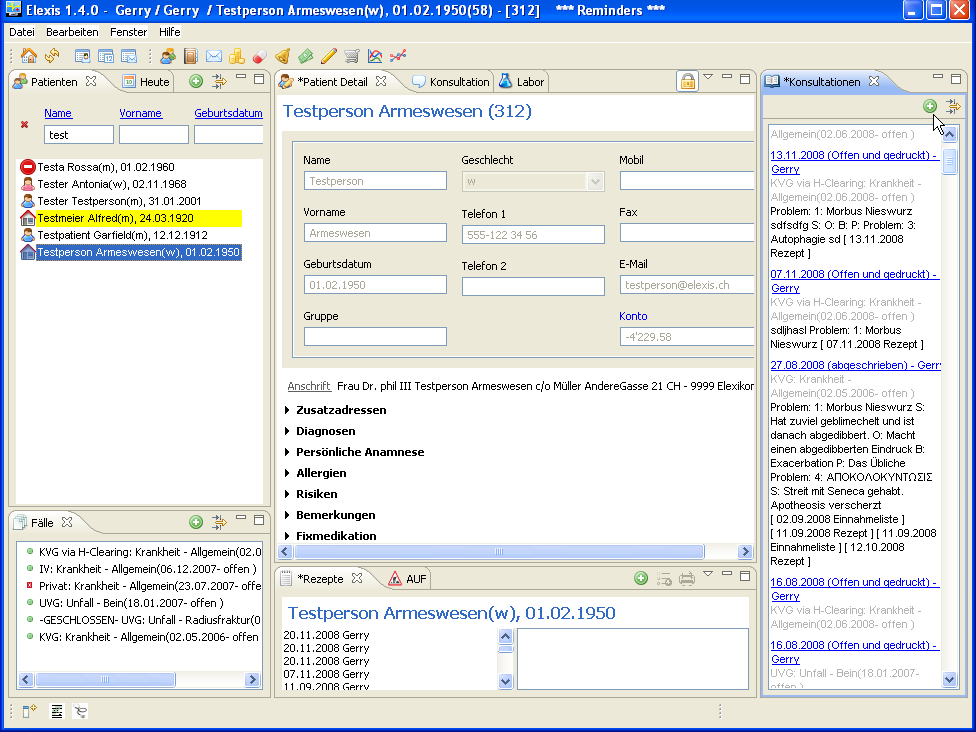
\includegraphics[width=0.9\textwidth]{images/einf0}
    %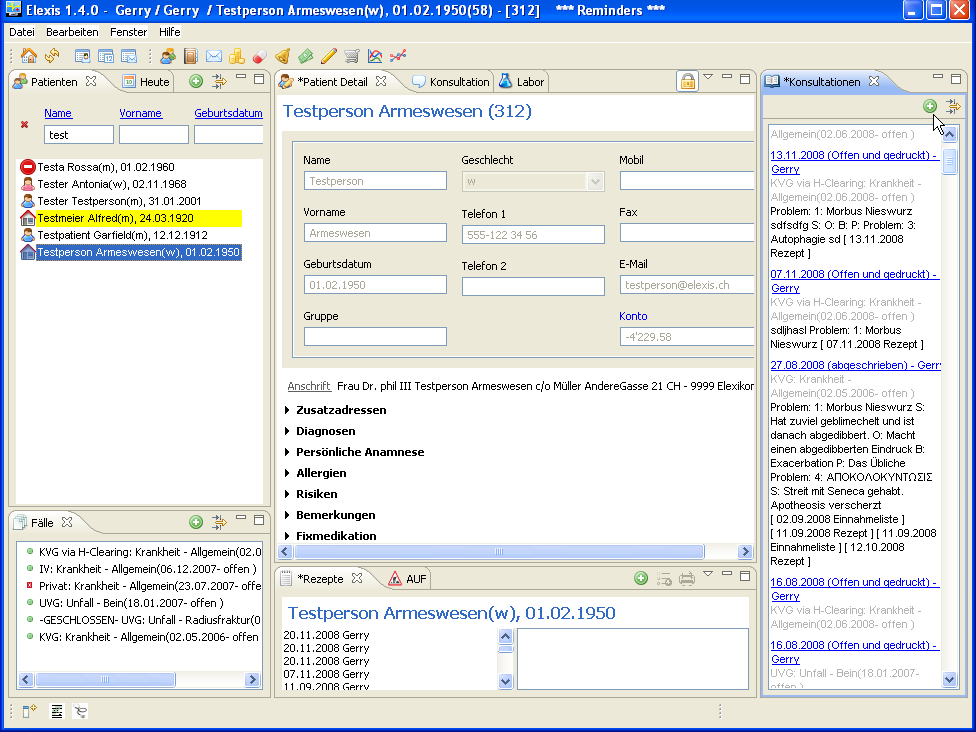
\includegraphics{images/einf0}
	\caption{Elexis Startbildschirm}
	\label{fig:startbild}
\end{figure}
\section{Patientendaten erfassen}
\begin{wrapfigure}{r}{8cm}
	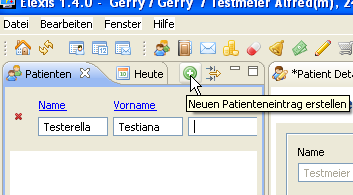
\includegraphics[width=6.5cm]{images/einf1}
	\caption{Patientennamen eingeben}\label{fig:patname}
\end{wrapfigure}
Aktivieren sie mit einem Klick die Ansicht 'Patienten' und schreiben Sie in die Eingabefelder Name und Vorname der neuen Patientin.
Falls die Patientin schon einmal erfasst worden ist erscheint ihr Name, in unserem Fall, wo keine Patientin dieses Namens vorhanden ist, werden unten keine Einträge angezeigt (s. Abb. \ref{fig:patname})\footnote{Um die Eingabefelder zu leeren und wieder alle Patienten anzuzeigen, können Sie auf das rote 'x' links neben den Eingabefeldern klicken.}.

\index{Patient!neu}
Klicken Sie dann auf das grüne Plus-Symbol oben rechts, um eine Patientin mit diesen
Daten neu anzulegen. Es erscheint ein Dialogfenster (Abb. \ref{fig:patdata}), wo
Sie die Angaben in die entsprechenden Felder eingeben können.\\
\bigskip

\begin{figure}[ht]
	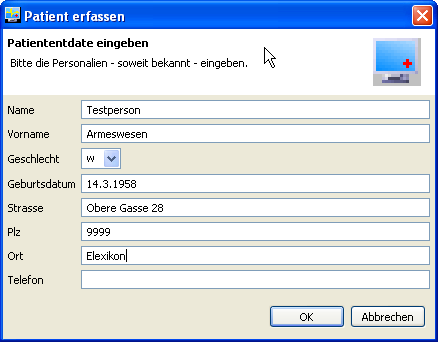
\includegraphics{images/einf2}
	\caption{Patientendaten ergänzen}
	\label{fig:patdata}
\end{figure}
Sie brauchen die hier verlangten Daten nicht vollständig einzugeben, sondern einfach soweit Sie diese im Moment kennen.
Sie müssen also im Notfalldienst nicht zuerst die vollständigen Daten eingeben, bevor Sie mit der Behandlung beginnen können.
Erfassen Sie z.B. nur Name und Geburtsdatum und überlassen Sie den Rest Ihrer MPA. Für Elexis ist ein neuer Patient in dem Moment bekannt,
wo Sie 'OK' klicken -- egal wieviele Daten zu diesem Zeitpunkt eingegeben sind.

\section{Falldaten erfassen}
Bei einer neuen Patientin müssen Sie zunächst einen \glqq Fall\grqq{} erstellen, dem
die Konsultation zugeordnet werden kann.
\index{Fall!erstellen}

\begin{figure}[htbp]
     \begin{minipage}{0.4\textwidth}
      \centering
       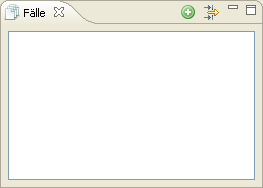
\includegraphics[width=0.8\textwidth]{images/einf3}
       \caption{Fälle-Ansicht}
       	\label{fig:faelle1}
     \end{minipage}\hfill
     \begin{minipage}{0.6\textwidth}
      \centering
       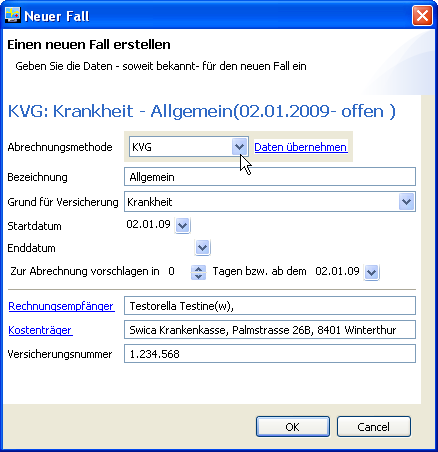
\includegraphics[width=1.0\textwidth]{images/einf4}
       \caption{Fall-Detail}
       \label{fig:falldetail}
     \end{minipage}
   \end{figure}


Ein Fall sammelt alle Konsultationen, die mit einem gemeinsamen Abrechnungssystem erfasst werden. (Vgl. \ref{settings:abrechnungssystem} auf S. \pageref{settings:abrechnungssystem}).
Klicken Sie also in der \glqq Fälle\grqq{}-Ansicht
(Abb. \ref{fig:faelle1}) auf das grüne Plus-Symbol.

Dadurch öffnet sich ein Dialog, in dem Sie wiederum die Angaben eintragen
können, soweit diese Ihnen bekannt sind (Abb. \ref{fig:falldetail})

Spätestens zur Rechnungsstellung müssen dann allerdings die notwendigen Angaben (Debitor, Kostenträger und Versicherungsnummer bzw. Fallnummer)
eingegeben werden.
Nach dem Klick auf OK haben Sie den neuen Fall erstellt. Bei weiteren
Konsultationen kann man sich diesen Schritt natürlich sparen.\\

\bigskip

Als nächstes erstellen wir eine neue Konsultation, wieder mit dem nun schon
bekannten grünen Plus-Symbol (Abb. \ref{fig:neuekons}.

\index{Konsultation!neu}
\begin{figure}[ht]
	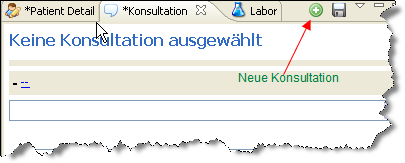
\includegraphics{images/einf5}
	\caption{Neue Konsultation}
	\label{fig:neuekons}
\end{figure}
\pagebreak[2]

Danach können wir mit dem KG-Eintrag beginnen (Abb. \ref{fig:KG}).

\section{Krankengeschichte führen}
\begin{figure}
    \begin{center}
	   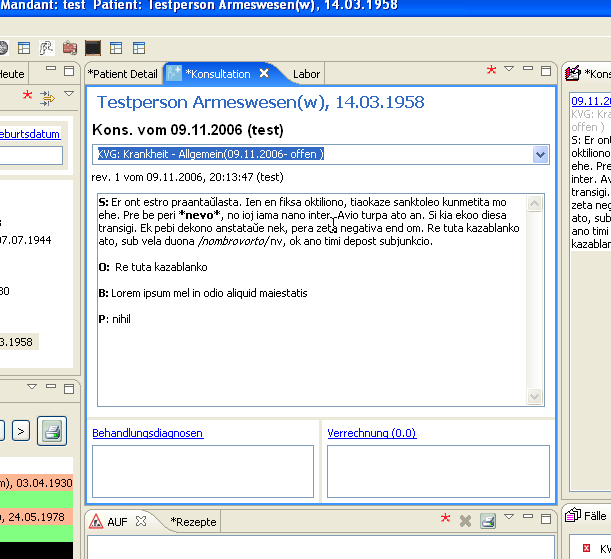
\includegraphics[width=0.7\textwidth]{images/einf6}
    	\caption{KG-Eintrag}
	   \label{fig:KG}
    \end{center}
\end{figure}
Der KG-Eintrag kann einfache Textformatierungen enthalten, Textbausteine können
beliebig definiert und über eine konfigurierbare shortcut-Taste aufgerufen werden. Die Verrechnung erfolgt dann entweder über ein Tastaturmakro oder per Maus.
Nach Fertigstellung des Eintrags (auch vor oder während des Eintragens) können
Sie durch Klicken auf \glqq Verrechnung\grqq{} die Leistungen-Ansicht öffnen
(Abb. \ref{fig:Verrechnung}). Analog können sie durch klicken auf
\glqq Behandlungsdiagnosen\grqq{} die Diagnosen-Ansicht öffnen.

\begin{figure}[ht]
	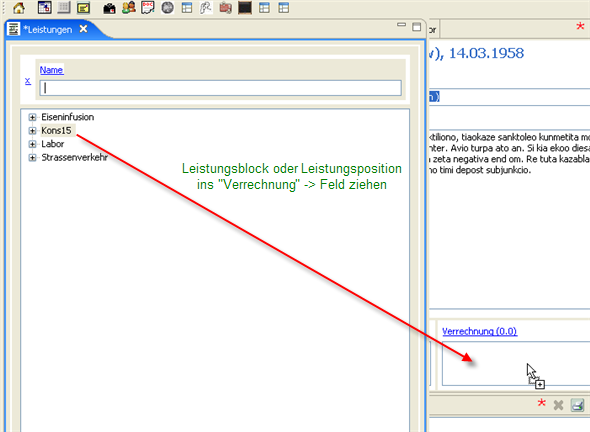
\includegraphics[width=6cm]{images/einf7}
	\caption{Verrechnungs-Fenster}
	\label{fig:Verrechnung}
\end{figure}
Dieses Fenster enthält alle im System vorgesehenen Leistungscode-Systeme, sowie eine Seite mit selbstdefinierten Leistungsblöcken.
\index{Leistungen!verrechnen}\index{abrechnen}
Sie können entweder einen ganzen Block oder einzelne Leistungen aus dem Block oder aus einem anderen Leistungsfenster (Tarmed etc.) ins \glqq Verrechnung\grqq{}-Feld ziehen (drag and drop).

Genau gleich lassen sich zur Konsultation auch Diagnosen zuordnen, auch hier hat man die Wahl zwischen allen im System integrierten Diagnosecodesystemen (beliebig anzupassen und erweiterbar).
\index{Konsultation!Diagnose}

\clearpage

\chapter{Benutzeroberfläche einrichten}
	\label{customize}
	% *******************************************************************************
% * Copyright (c) 2007-2008 by Elexis
% * All rights reserved. This document and the accompanying materials
% * are made available under the terms of the Eclipse Public License v1.0
% * which accompanies this distribution, and is available at
% * http://www.eclipse.org/legal/epl-v10.html
% *
% * Contributors:
% *    G. Weirich - initial implementation
% *
% *  $Id: customize.tex 4896 2009-01-02 08:23:59Z rgw_ch $
% *******************************************************************************
% !Mode:: "TeX:UTF-8" (encoding info for WinEdt)

\section{Principe de fonctionnement}
La caractéristique frappante de Elexis est sa grande flexibilité. Si vous êtes habitué à un
autre logiciel, l'utilisation de Elexis peut vous apparaître un peu inhabituel. Pour cette raison nous allons tout d'abord expliquer quelques concepts de base.

\index{Principe de fonctionnement}
 \subsection{Bureau / Perspective}
 \index{Perspective}\index{Affichage}\index{View}
Imaginez votre table de travail. Vous vous êtes probablement habitué de poser certaines choses à un endroit spécifique sur votre bureau, c'est-à-dire attribuer certaines fonctions de travail à un lieu, où vous pouvez (idéalement) les retrouver facilement. Votre ordre n'est pas nécessairement le même que pour quelqu'un d'autre qui a le même modèle de bureau.
La fenêtre du programme Elexis est comme un bureau (voir fig. \ref{fig:tour1}. Il n'est en aucun cas préfixé à quel endroit une fonction spécifique doit être située et il n'est même pas définie,
lesquels des éléments doivent apparaître sur le bureau et lesquels peuvent rester rangés quelque part dans un tiroir pour être sortis seulement en cas de besoin.


%\usepackage{graphics} is needed for \includegraphics
\begin{figure}[htp]
\begin{center}
  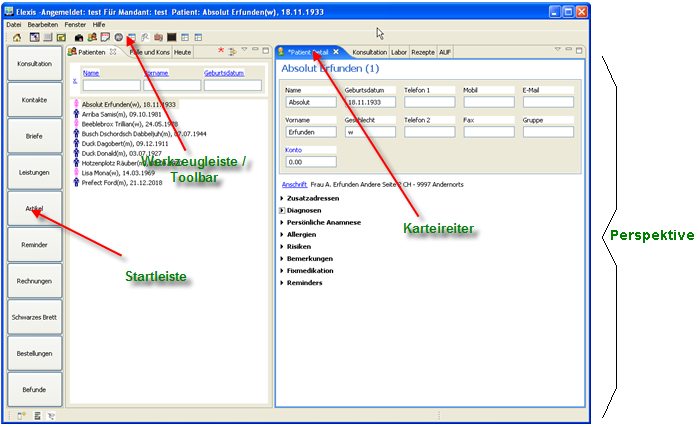
\includegraphics[width=0.9\textwidth]{images/tour1}
  \caption{Standard-Perspektive}
  \label{fig:tour1}
\end{center}
\end{figure}

Un aménagement de surface de travail nous appelons une 'perspective' (perspective). On appelle 'Affichage' (view) les différentes sous-fenêtres respectivement les sous-unités (comme en haut 'patients' et 'détails du patient') qui composent la perspective.

\subsubsection{Perspectives et views}

La (fig. \ref{fig:tour1} montre un exemple de perspective appropriée pour un petit écran.
Il affiche une capture d'écran sur un TFT 15 pouces. Les affichages \glqq
patients\grqq{}(à gauche) et \glqq détails du patient\grqq{}(à droite) se trouvent au-dessus d'autres affichages dont on ne voit que les onglets.

Sur un écran plus grand on favoriserait probablement un autre aménagement : fig. \ref{fig:tour2} montre une capture d'écran sur un TFT 17 pouces avec plusieurs views en même temps.

%\usepackage{graphics} is needed for \includegraphics
\begin{figure}[htp]
\begin{center}
  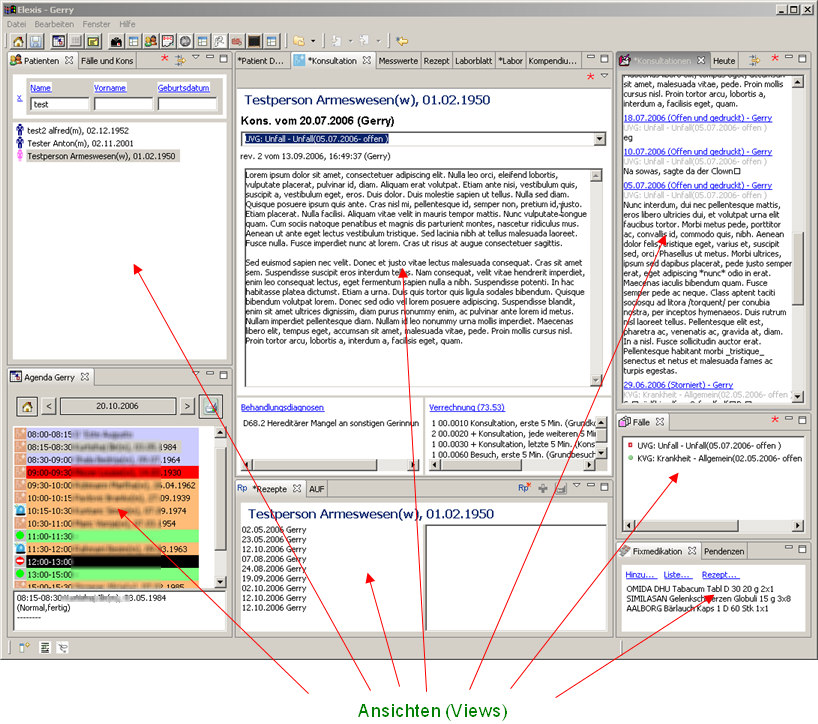
\includegraphics[width=0.9\textwidth]{images/tour2}
  \caption{Komplexere Perspektive}
  \label{fig:tour2}
\end{center}
\end{figure}

\subsubsection{Affichage / views}
Chaque affichage correspond à une fonctionnalité spécifique. Dans cette fenêtre (fig. 4.2)
on voit une liste de patients (à gauche) et les 'détails du patient' actuellement actif (à droite).
Il y a d'autres affichages comme 'Consultation' qui permet l'introduction des informations médicales dans le dossier du patient, 'l'Historique' qui est un listing de toutes les notes faites dans le dossier du patient, la 'Médication fixe', les 'Ordonnances', les 'Certificats' d'incapacité de travail, 'l'Agenda' et autres.
Chaque affichage est une  \glqq vue\grqq définie sur des données existantes. Il peut être activé en cliquant sur l'onglet.  Les onglets eux-mêmes peuvent être disposées, activés ou désactivés au choix.

Peu importe la façon dont vous avez ordonné les affichages, vous pouvez les voir à tout moment à plein écran pour une meilleure vue d'ensemble, en double-cliquant sur l'onglet. Un double-clic sur l'onglet permet l'affichage en mode plein écran et un autre double-clic le remet à l'endroit d'origine.
(cf Fig. \ref{fig:tour3}).

\begin{figure}[htp]
\begin{center}
  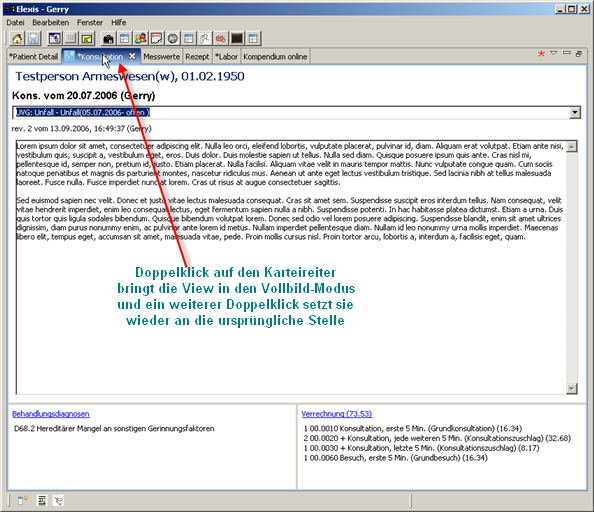
\includegraphics[width=0.9\textwidth]{images/tour3}
  \caption{View maximieren}
  \label{fig:tour3}
\end{center}
\end{figure}

\subsubsection{Aménager views et perspectives}


Dans la perspective de démarrage par défaut on trouve à gauche une \glqq barre de démarrage \grqq{}. Celle-ci vous amène à des perspectives prédéfinies dans lesquelles vous trouvez les affichages appropriés.
La barre d'outils mène, comme d'habitude pour d'autres programmes, à des différents fonctions. Chaque affichage a un onglet. Par un clic sur cet onglet l'affichage peut être mis au premier plan ou il peut être maximisé par un double clic comme déjà mentionné

\par
\clubpenalty=5000
\medskip
Le contenu des fenêtres du programme et les compilations des affichages peuvent être facilement adaptés à vos besoins:\\

\begin{itemize}
  \item Vous pouvez supprimer des affichages dont vous n'avez pas besoin pour gagner de la place pour les affichages restants.
	\item Vous pouvez agrandir ou réduire la taille des affichages à l'horizontale et à la verticale.
	\item Vous pouvez déplacer les affichages à n'importe quel endroit sur l'écran (en \glqq maintenant enfoncé\grqq{}la touche gauche de la souris sur l'onglet de l'affichage en question '=drag and drop'  )
\end{itemize}

Chaque composition peut être enregistré en tant que perspective - et reste en tant que telle
facilement accessible.


\subsection{Aménager et sauvegarder des perspectives}
\label{tour:customize}
Vous ne pouvez pas seulement créer une seule perspective, mais autant que vous voulez. Votre assistante médicale aura peut-être besoin d'une autre perspective que vous-même, par exemple, elle souhaite avoir l'agenda en plein écran. Vous même, vous pouvez utiliser des différentes perspectives, par exemple une pour les consultations et une autre pour la comptabilité ou si vous devez écrire un rapport.
Dans Elexis des nouvelles perspectives peuvent être composées facilement:\\

\bigskip

\textbf{Premier pas : Ouvrez l'affichage (les affichages) souhaité}\\

Cliquez dans le menu  \textsc{WINDOW - PERSPECTIVE sur OTHER}. Une boite de dialogue s'ouvre. Voir Fig. \ref{fig:cust1}.\\

\begin{figure}[htbp]
   \begin{minipage}{0.4\textwidth}
       \centering
       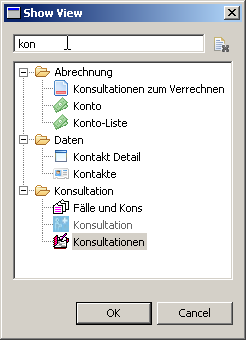
\includegraphics[width=0.8\textwidth]{images/customize1}
       \caption{View suchen}
       \label{fig:cust1}
     \end{minipage}\hfill
     \begin{minipage}{0.5\textwidth}
        Cette boîte de dialogue vous montre tous les affichages disponibles dans l'installation de votre Elexis. (Lesquels et combien ils sont est dépendant des plugins installés). La liste sera automatiquement filtrée, si vous tapez dans la première ligne de cette boite de dialogue le début du nom de l'affichage cherché.

        Si vous ne connaissez pas le nom de l'affichage cherché vous pouvez aussi parcourir tous les affichages.

    \end{minipage}
\end{figure}

\bigskip
\pagebreak[3]
\textbf{Deuxième pas : Déplacer les affichages à l'endroit souhaité et choisir sa taille :}\\

   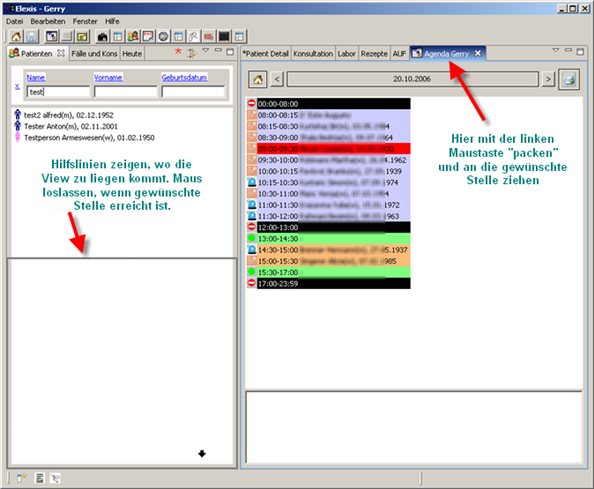
\includegraphics[width=0.8\textwidth]{images/agendagewaehlt}
Une ligne supplémentaire indique où l'affichage se trouvera. Relâchez la souris lorsque la position désirée est atteinte.
Saisir ici avec le bouton gauche de la souris et tirer à l'endroit souhaité. (drag and drop)
Si la flèche de la souris se trouve entre deux affichages (vertical ou horizontal), elle est est transformée en flèche double et peut ensuite déplacer la frontière entre les deux affichages.

   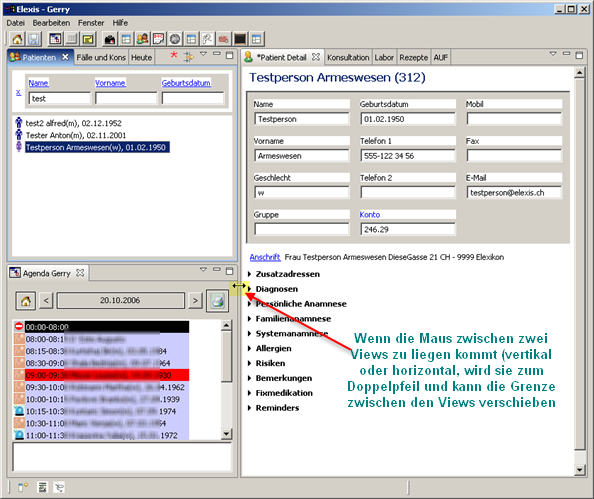
\includegraphics[width=0.8\textwidth]{images/agendaanpassen}

\bigskip
\textbf{Troisième pas : Sauvegarder la perspective}\\
\index{Sauvegarder la perspective}
Si vous souhaitez que votre perspective ainsi établi soit aussi disponible lors d'un démarrage ultérieure ou sur d'autres ordinateurs vous avez plusieurs possibilités :
\begin{itemize}
\item Sélectionnez dans le menu  \textsc{FENÊTRE - PERSPECTIVE - SAUVEGARDER COMME PERSPECTIVE DE DEPART}. Ainsi, vous déterminez que cette perspective apparaisse désormais lors du démarrage.
\item \textsc{FENÊTRE - PERSPECTIVE - SAUVEGARDER COMME …}. Vous avez ainsi la possibilité de sauvegarder la perspective actuelle sous un nom quelconque. Sachant le nom de la perspective, vous pouvez la récupérer à une date ultérieure avec  \textsc{FENÊTRE - PERSPECTIVE - AUTRES...}.
\item \textsc{FENÊTRE - PERSPECTIVE - SAUVEGARDER}. Dans ce cas la perspective actuelle est sauvegardée sous le nom actuel.
\item And last but not least : Si vous sauvegardez sous \textsc{FICHIER - REGLAGES - UTILISATEUR} la perspective sous un certain nom, vous pouvez l'utiliser aussi depuis un autre ordinateur sous le même nom\footnote{Ceci n'est naturellement possible que si sur le poste concerné tout les affichages existent, dont on aura besoin dans cette perspective}. Cette option est idéale pour créer un environnement de travail homogène.
\end{itemize}

\textbf{Ou : réinitialiser la perspective}\\
\index{réinitialiser la perspective}
Si les modifications ne vous conviennent quand même pas, ou si vous avez fermé
par exemple par erreur un affichage, vous pouvez tout simplement retourner
à la version de la perspective actuelle enregistrée : Choisissez dans le menu
\textsc{FENÊTRE - PERSPECTIVE - RECONSTITUER.} Ceci n'est naturellement possible que, tant que
vous n'avez pas stocké vos modifications.(troisième pas).




%%%%%%%%%%%%%%%%%%%%%%%%%%%%%%%%%%%%%%%%%%%%%%%%%%%%%%%%%%%%%%%%%%%%%%%%%%%%%%%
\part{Systematische Referenz}
\chapter{Konzepte}
	% *******************************************************************************
% * Copyright (c) 2007-2008 by Elexis
% * All rights reserved. This document and the accompanying materials
% * are made available under the terms of the Eclipse Public License v1.0
% * which accompanies this distribution, and is available at
% * http://www.eclipse.org/legal/epl-v10.html
% *
% * Contributors:
% *    G. Weirich
% *
% *  $Id: konzepte.tex 5231 2009-04-02 13:16:56Z rgw_ch $
% *******************************************************************************
% !Mode:: "TeX:UTF-8" (encoding info for WinEdt)

\section{Contacts}
\label{kontakt}
\index{contact!définition}
Dans Elexis, chaque personne ou entreprise qui est dans une relation avec le cabinet, est
tout d'abord un\glqq contact\grqq{}. La saisie ou la modification des contacts se fait dans la perspective de contact.
\begin{flushleft}
    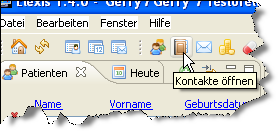
\includegraphics{images/contactperspective}
\end{flushleft}


Ils existent les types de contact suivants :
\begin{itemize}
  \item personne
	\begin{itemize}
  		\item mandant
  		\item utilisateur
  		\item patient
  		\item autres
    \end{itemize}
    \item{oganisation}
    \begin{itemize}
      \item{laboratoire}
      \item {autres}
    \end{itemize}
\end{itemize}


\section{Utilisateurs et Mandants}
\index{utilisateur!définition}\index{mandant!défintion}
Quelqu'un qui a le droit de facturer ses prestations à charge de l'assurance obligatoire de soins (ce qui est en Suisse seulement possible si on a son propre numéro de concordat RCC ), est un \textit{mandant}. Chaque processus dans Elexis (consultation, laboratoire, prescription etc.) se passe toujours sous la responsabilité et sur le compte précisément d'un Mandant. \index{mandant}

\medskip

JQuelqu'un qui peut manier le programme , est un \textit{utilisateur}. Un utilisateur travaille toujours sur ordre d'un Mandant spécifique.

Ainsi il existe à chaque moment dans Elexis un Mandant actuel et un utilisateur actuel.
\index{utilisateur}Mandant und Anwender können auch identisch sein (Wenn der
Mandant selbst am PC arbeitet).
Le Mandant et l'utilisateur peut aussi être identique (si le Mandant lui-même travaille au PC). Un utilisateur peut aussi modifier l'attribution à un Mandant (si une assistante médicale dans un cabinet de groupe travaille par exemple pour des Mandants différentes).
\index{groupes}\index{droits}
\index{droits}\index{utilisateur!droits}
Des utilisateurs ont certains droits individuellement réglables, avec lesquels on peut contrôler très finement à qui on permet quelles actions dans Elexis. Des utilisateurs peuvent aussi être rassemblés dans des groupes qui définissent certains droits communs (p. ex. groupes  \glqq assistantes médicales\grqq{} ou \glqq médecins\grqq{}). Le groupe \glqq Admin\grqq{}: est un groupe spécial : Celui qui fait partie de ce groupe, a automatiquement  \textit{tous} les droits.

\medskip

\textbf{Important}: Même si cela peut d'abord vous apparaître illogique : Aussi le chef ne devrait pas travailler habituellement comme Admin \index{administrateur}.
La raison se trouve dans le fait que l'Admin-Account permet aussi des suppressions irréversibles et d'autres modifications très désagréables. Dans l'état fiévreux du quotidien on risque facilement de cliquer une fois sur le faux bouton !
Par conséquent : Travaillez dans le quotidien avec un Account qui donne précisément les droits dont vous avez besoin au quotidien. Etablissez un deuxième Account pour vous,celui qu'est assigné au groupe Admin, et ne vous annoncez sous cet Account que lorsqu'il est vraiment nécessaire.

Le concept des groupes et droits est expliqué plus précisément à partir de la page\pageref{sec:gruppen} .

\section{Consultations, cas, garants et répondant des coûts}
\index{consultation!définition}\index{cas!définition}\index{facturation} Chaque contact retenu dans les Elexis entre le personnel du cabinet et un patient est une  \textit{consultation}. Lorsqu'une consultation est comptabilisé la facturation sera faite en faveur du Mandant, pour lequel l'utilisateur connecté a travaillé.
\label{definition:fall}
Chaque consultation est aussi assignée à un \textit{cas}. Ein Fall ist hier eher eine versicherungstechnische, als eine medizinische Einheit: Un cas est ici plutôt une entité assécurologique qu'une entité médicale : Le cas rassemble toutes les consultations qui sont comptabilisées avec le même système de facturation (voir\ref{settings:abrechnungssystem}à la page \pageref{settings:abrechnungssystem}). Cela peut parfois être identique avec la notion de cas médical (un accident qui est facturé à un assureur spécifique avec un numéro de cas spécifique), ou ne peut pas avoir de lien avec un cas médical  (p. ex. en général en Suisse un cas de maladie sera subsumé à la \glqq maladie\grqq{} qui rassemble toutes les consultations LAMAL).

Un cas ne peut être attribué à qu'un seul patient et un système, mais peut toutefois comprendre des consultations de plusieurs Mandants. (Une facture distincte est alors fournie pour chaque Mandant).

\section{Sticker}
\index{stickers}\index{étiquettes}\index{marquage}
\label{Etiketten}
Des patients et d'autres contenus de base de données peuvent être marqués avec des 'stickers' (étiquettes). Un 'sticker' est une caractéristique en principe arbitraire qui est liée avec un objet correspondant de la base de données. Par exemple un patient pourraient être marqué avec le 'sticker' 'modèle de médecin de famille', 'MRSA' ou autre. Un tel 'sticker' est affichée lors de l'appel de l'objet correspondant.

 Des 'stickers' sont définis sous \textsc{Fichier-Paramètres-Sticker} (page Fig. \ref{fig:etiketten1}). ELa quantité des stickers peut être définie au choix. Pour créer un nouveau sticker, écrivez le texte pour le sticker dans le champ en haut et cliquez sur 'nouveau sticker'. Le 'sticker' que vous venez de créer apparaît alors avec des valeurs standards sur la liste des stickers. Sélectionnez le sticker et suggérez une image (format 16x16 tout au plus à 32x32 pixels), une couleur de texte et une couleur d'arrière-plan.
L'importance de la  'valeur' vous est expliquée ci- dessous.


\begin{figure}
    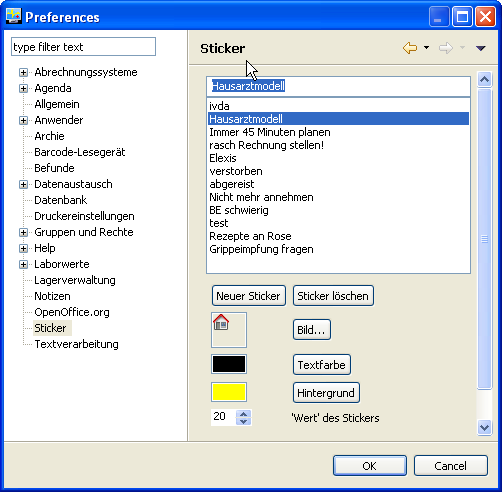
\includegraphics{images/etikette1}
    \caption{Sticker erstellen}
    \label{fig:etiketten1}
\end{figure}

Des stickers crées de cette façon peuvent être attribués à un patient qui se trouve sur la liste des patients par un clic sur la touche droite de la souris ce qui permet de choisir un 'Sticker' sur un menu déroulant. On peut attribuer à chaque patient entre zéro et x 'stickers'. On trouvera dans la liste des patients la saisie correspondante avec les 'stickers' et images, couleur du texte et couleur d'arrière plan.  (Fig. \ref{fig:etiketten2}).
\begin{figure}
    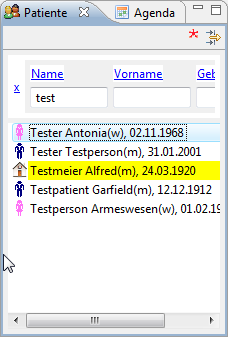
\includegraphics{images/etikette3}
    \caption{Anzeige der Sticker}
    \label{fig:etiketten2}
\end{figure}

Ici, on voit alors aussi le sens de l'attribut 'valeur' d'un sticker:
Lorsqu'un patient a reçu plusieurs stickers assignés, la liste des patients indique toujours
celui avec  'la valeur' la plus élevée. Les chiffres que vous utilisez là concrètement n'ont pas d'importance car la valeur absolue ne joue pas de rôle, par contre les relations entre les 'valeurs'.


\medskip

Si vous ouvrez une consultation pour y faire vos notes, vous y voyez toutes les stickers assignées au patient.
\begin{figure}
    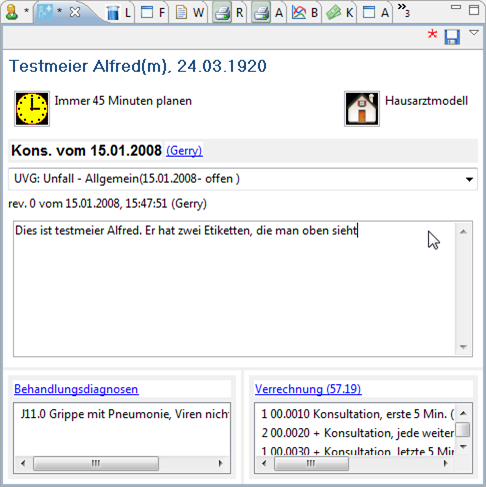
\includegraphics{images/etikette2}
    \caption{Konsultation mit Stickern}
    \label{fig:etiketten3}
\end{figure}


\clearpage

\section{Décompte des prestations}
\label{concept:leistung}
\index{Codes de prestation}\index{faire les comptes}
\begin{wrapfigure}{l}{7.5cm}
    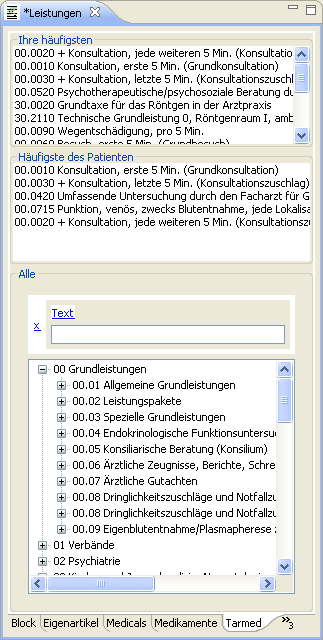
\includegraphics[width=7.5cm]{images/leistungen1}
    \caption{Leistungen}
    \label{fig:leistungen}
\end{wrapfigure}
\index{prestation!comptabiliser}
Les codes de prestations qui peuvent être comptabilisé, sont fournis d'une part par les Plugins (p. ex. par Elexis-tarif médical-Suisse), d'autre part par des blocs de prestations définis par vous-même (voir ci-dessous).
Vous trouvez tous les systèmes de codage de prestations existants sous la fenêtre
\glqq prestations\grqq{} (Fig. \ref{fig:leistungen}): Vous voyez au bord inférieur de la fenêtre un onglet pour chaque système de codage installé. 
Cette fenêtre apparaît lorsque vous cliquez depuis la fenêtre de consultation sur
 \glqq{}saisie prestations\grqq{}. La structure est la même pour chaque système de codage de prestations :

La fenêtre partielle supérieure montre les codes les plus fréquemment appliqués par vous dans ce système de codage de prestations, chose qui vous permet un accès rapide sans chercher longtemps. La liste est mise à jour régulièrement et plus vous utilisez un certain code, plus haut dans la liste il apparaîtra lors de la prochaine ouverture de la fenêtre.


\medskip
Dans la partie moyenne, les codes jusqu'ici utilisés les plus fréquemment pour ce patient apparaissent triés selon
le même principe. La fenêtre partielle la plus basse met à disposition le système de codage de prestation entier
avec toute sa systématique.


\bigskip

Pour introduire un code de prestation, vous pouvez le tirer d'une des trois sections de la fenêtre de 'prestations' dans la fenêtre de 'saisie prestations' ou le choisir par double-clic.
Certains Plugins peuvent contenir un  \glqq Optifier\grqq (Optimizer/Verifier) qui reconnaît des erreurs et/ou peut appliquer des corrections. Ainsi refuse par exemple le Tarmed- Plugin d'une part la facturation double du code \textit{00.0010 Consultation 5 premières minutes } avec un message d'erreur  (Verifier), et d'autre part il ajoute automatiquement le code 00.0010 lorsque vous introduisez le code 00.0030 \textit{00.0030 Consultation 5 dernières minutes} car 00.0030 se combine toujours avec 00.0010 (Optimizer).
Les\textit{articles}, qui sont remis directement au patient peuvent aussi être comptabilisés directement depuis cette fenêtre et leur stock est automatiquement ajusté.

\subsection{Blocs de prestations et prestations propres}
\begin{wrapfigure}{r}{6cm}
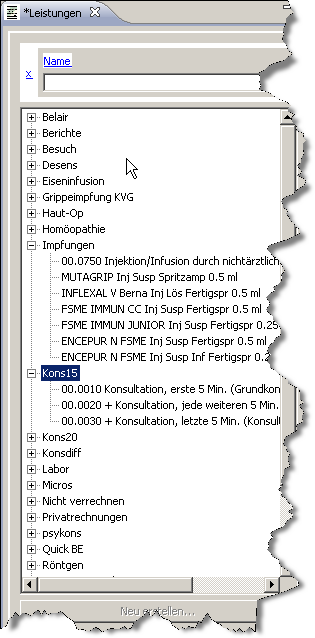
\includegraphics{images/block1}
\caption{Leistungsblöcke}
\label{fig:bloecke}
\end{wrapfigure}
\index{prestations propres}
\index{blocs de prestations}
Comme autre allègement du travail Elexis permet aussi de résumer plusieurs codes de prestation dans des blocs de prestation qui seront comptabilisé entièrement ou partiellement, et ceci même si ces blocs proviennent des systèmes de codage de prestation tout à fait différents. A part des blocs de prestations de provenance des systèmes de codage de prestations pré installés, de tels blocs peuvent contenir aussi des éléments à comptabiliser définis par vous même.
Vous voyez dans la Fig.\ref{fig:bloecke} quelques exemples :\textit{cons15} est un exemple de bloc qui est comptabilisé
généralement en bloc. Pour ce faire vous pouvez, tirer le bloc avec la souris dans la fenêtre de saisie de prestation de la consultation ou, si vous travaillez plutôt avec le clavier, vous tapez le nom du bloc, suivi de la clé de libération des macros dans le texte de consultation
(conformément aux normes c'est le \#). L'entrée de cons15\# dans le texte de consultation comptabiliserait ainsi dans notre exemple une consultation de 15-minutes selon tarif Tarmed.
\textit{Les Vaccinations} seraient un exemple de bloc, qui serait plutôt pensé comme sommaire d'éléments semblables
(avec le but d'un gain de temps pour trouver plus rapidement l'élément cherché) qui seront de toute façon comptabilisé
séparément. Dans ce cas, on tire simplement les différents éléments du bloc dans la fenêtre de saisie de prestation .


Pour créer un nouveau bloc, on introduit (à libre choix mais toutefois unique) un nom pour ce bloc et clique ensuite sur \textit{créer nouveau ...}. Les prestations s'ajoutent au bloc dans la fenêtre des codes(voir  Fig. ref{fig:bloecke2}).
\begin{figure}[htp]
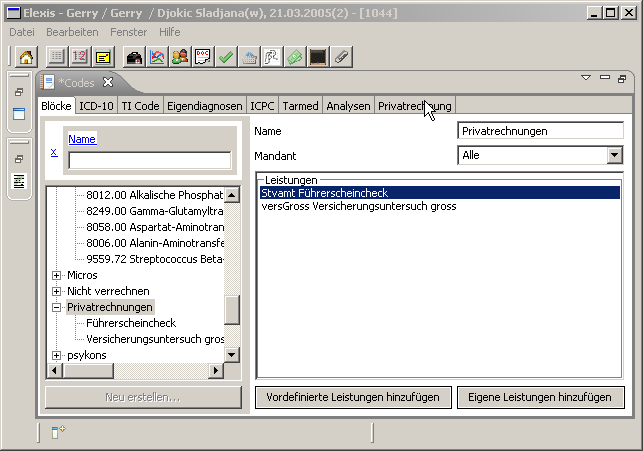
\includegraphics[width=0.9\textwidth]{images/block2}
\caption{Leistungsblock definieren}
\label{fig:bloecke2}
\end{figure}
Vous pouvez ajouter par drag\&drop soit des prestations prédéfinies de provenance d'un des systèmes de code installés, soit définir vos propres prestations. Ici vous devez aussi indiquer frais et prix en centimes/cents ainsi que le temps budgétisé pour la prestation en minutes.


\section{Articles et stocks}
\index{article}\index{médicament}\index{stock}
 Tout ce qui peut être acheté, stocké, livré ou prescrit est un  \textit{article}.
 Les articles sont organisés dans des classes par exemples classes au \textit{médicaments},
 ou à des  \textit{LiMA} ou au\textit{matériel bureautique}.
 Elexis peut adopter chaque article qui lui est connu comme \textit{article en stock}.

 Un article en stock est un article dont l'existence est contrôlée et qui peut être commandé si nécessaire de façon semi-automatique. Des plus amples informations concernant les articles et leur stockage se trouvent dans la description de la View (à la page \pageref{view:artikel} et suivantes.)

\section{Importation des données externes }
\index{importation}
En principe Elexis est en mesure d'importer des données de n'importe quelle source .
Toutefois, le format de ces données doit naturellement être connu ou standardisé d'une certaine manière. Par conséquent l'importation de données est en générale effectué par les 'Importer-Plugins'.
Il y existent des 'Importers' pour des données d'annuaire téléphonique, pour les bases de données d'autres programmes pour le cabinet médical, pour des laboratoires externes, pour des appareils de laboratoire et pour d'autres appareils médicaux qui sont capables de transférer leurs données sur un ordinateur, pour des LiMA, des médicaments,
le Tarmed et d'autres bases de données etc.
Vous trouvez une liste de Plugins disponibles dans le menu 'Plugins' sur  http://www.elexis.ch. Des 'Importers' supplémentaires peuvent être programmés assez facilement, en cas de besoin vous pouvez nous contacter pour demander un devis.

\medskip

Les 'Importers' se trouvent généralement dans le menu local des 'Views' qui affichent les données correspondantes (p. ex. Tarmed-Importer ou Importer du laboratoire). Une classe d' 'Importers' qui ne sont pas attribués à certaine 'View' se trouvent aussi dans le menu d' 'importation de données' sous 'Fichier' dans la barre de menu. Ici, un dialogue s'ouvre comme dans la fig. \ref{fig:importdlg}.
\begin{figure}
  % Requires \usepackage{graphicx}
  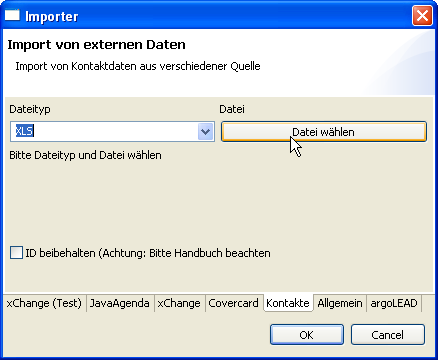
\includegraphics{images/importdlg}\\
  \caption{Import-Dialog}\label{fig:importdlg}
\end{figure}
\index{Import!contacts}
Dans les onglets en bas de la fenêtre vous trouvez tous les 'Importers' de base installés. Lesquels s'y trouvent dépend des Plugins installés. Seulement le 'Contact-Importer' qui est choisi dans l'illustration existe toujours. Cet 'Importer' peut importer des contacts des fichiers externes, pour autant que ceux-ci soient préparés de façon standardisée en forme de tableaux. Choisissez sous 'le type de fichiers' s'il s'agit d'un tableau Microsoft\texttrademark Excel\texttrademark(xls), d'un tableau Caracter Separated Values (csv) ou d'un tableau de Santésuisse contenant les assureurs et leurs codes EAN.
S'il s'agit de xls, le fichier doit contenir un tableau 0 avec les colonnes suivantes :


\begin{tabular}[h]{|l|l|}
\hline Titre de colonne & Légende\\
\hline
\hline  ID & une identification (en principe au choix mais univoque dans le fichier)\\
\hline Istpersonne & 1 si la saisie concerne une personne, 0 pour tout les autres cas (organisations etc)\\
\hline Istpatient & 1 si la saisie concerne un patient, 0 pour tout les autres cas\\
\hline titre & titre, personne de référence etc.\\
\hline désignation1 & En cas d'une personne son nom de famille\\
\hline désignation2 & En cas d'une personne son prénom\\
\hline supplément & \\
\hline date de naissance & En format dd.mm.yyyy ou yyyy-mm-dd\\
\hline genre & m ou f ou un mot qui commence avec m ou f\\
\hline e-Mail & adresse E-Mail\\
\hline website & une adresse WWW\\
\hline téléphone 1 & Numéro de téléphone primaire\\
\hline téléphone 2 & Numéro de téléphone supplémentaire\\
\hline mobil & Numéro de téléphone portable\\
\hline rue & Rue et numéro de maison\\
\hline code postal & code postal écrit comme 1224 ou comme CH-1224 (doit être formaté comme fichier texte)\\
\hline localité & \\
\hline adresse & Adresse comme elle apparaîtra sur une étiquette d'adresse. Nouvelle ligne par $\backslash$n\\
\hline EAN & Code EAN comme EAN13\\
\hline
\end{tabular}

\medskip

Pour que le format puisse être reconnu la première ligne du tableau doit contenir les titres de colonne précisément dans la forme de présentation ci-dessus. Chacune des colonnes citées doit exister mais peut toutefois être vide. Le fichier doit donc être codé comme iso-8859-1 (c'est une norme sous Windows ; avec la version MAC de Excel, le codage d'exportation devrait en conséquence éventuellement être adapté).


\medskip

Si vous avez fixé le type de fichier, cliquez vous sur le bouton 'choisir fichier' et cherchez le fichier à importer. Ne placez un crochet à 'préserver ID' seulement 
 \textbf{seulement},lorsque \begin{itemize}
\item chaque paquet de données dans le champ ID a une ID 
\item cette ID est univoque, et ne peut donc entrer en collision avec aucun autre contact dans Elexis
\item il est indispensable de maintenir cette ID.
\end{itemize}
Si vous ne placez pas le crochet, chose qui est recommandée dans la plupart des cas, alors Elexis fournira lors de l'importation une identité univoque pour chaque contact (comme si on introduisait manuellement ce contact).\\
Cliquez alors OK, pour commencer l'importation.

 \section{Plusieurs instances simultanément}
 \index{simultanément}
 Vous pouvez démarrer Elexis sans problèmes plusieurs fois simultanément pour afficher dans les fenêtres des perspectives différentes ou différents patients.
Certains éléments peuvent aussi être échangés par Cut\&Paste entre les instances courantes. Exemples d'application :

 \begin{itemize}
   \item Vous travaillez sur une entrée de patient et vous recevez un appel téléphonique  concernant un autre patient. Au lieu de quitter votre travail vous cliquez sur l'Elexis qui est ouvert en arrière plan et cherchez le dossier de ce patient.
   \item A son poste de travail votre assistante médicale voudrait avoir en même temps l'agenda et les données des patients à portée de vue. Si vous lui payez un deuxième écran (au lieu d'un deuxième PC), vous attachez les deux écrans au même PC à une carte graphique DualHead et mettez sur chaque écran une instance propre de Elexis.
   \item Pendant que l'Elexis est occupé à faire la facturation qui prend du temps, vous ne voudriez pas glander. Sans problème, vous démarrez une deuxième instance d'Elexis et continuez à travailler. (Vous pourriez naturellement aussi aller boire un café ou faire une promenade).
   \item Vous écrivez une lettre, mais vous aimerez y mettre certaines parties d'une autre lettre.
Ouvrez dans une instance d'Elexis l'ancienne lettre, copiez là certains passages et collez les dans l'autre lettre que vous êtes en train d'écrire dans l'autre instance d'Elexis.

 \end{itemize}

\section{Plugins}
\index{Plugin!définition}
Ce concept est discuté en détail à la page \pageref{expl:plugins}. Ici mentionnons pour le moment seulement : Elexis est extensible dans tout les sens. Il n'y a pas seulement un certain nombre de \glqq modules\grqq{} mais en fait, à tout moment, des nouvelles fonctions peuvent être programmé dont lors du lancement de la version actuelle on n'avait pas encore connaissance. Cela se fait sous forme de \glqq Plugins\grqq{}. Les 'plugins' peuvent être programmés par exemple pour, de la statistique, la comptabilité, l'importation de données de laboratoire, l'accessibilité des
appareils, l'exportation des données du dossier médical, des nouveaux systèmes de comptabilisation des prestations, des nouveaux systèmes de classifications des diagnostics etc.
Donc un 'Plugin' est dans Elexis simplement un programme avec des capacités au choix qui a la propriété de pouvoir coopérer avec Elexis.
Il est impossible de présenter ni dans ce guide ni ailleurs une liste exhaustive de tous les 'Plugins' parce que personne ne peut savoir quels 'Plugins' ont été commandés par des usagers indépendants auprès des programmeurs indépendants.
Un listing de tout les 'Plugins' qui nous sont connus se trouve sur : http://www.elexis.ch




\chapter{Menü und Toolbar} 					
	% *******************************************************************************
% * Copyright (c) 2007 by Elexis
% * All rights reserved. This document and the accompanying materials
% * are made available under the terms of the Eclipse Public License v1.0
% * which accompanies this distribution, and is available at
% * http://www.eclipse.org/legal/epl-v10.html
% *
% * Contributors:
% *    G. Weirich - initial implementation
% *
% *  $Id: menu.tex 4903 2009-01-03 11:44:22Z rgw_ch $
% *******************************************************************************
% !Mode:: "TeX:UTF-8" (encoding info for WinEdt)

% Dieses Dokument enthält die Dokumentation der Menübefehle

\section{Menu}
Le menu est - comme la plupart des éléments d'Elexis- pas fixe. Les Plugins peuvent ajouter des propres commandes de menu ou des sous-menus entiers. Ce qui suit ne décrit par conséquent que le contenu des menus qui existent dans l'installation de base de Elexis.

\begin{itemize}
  \item {\textsc{fichier -- utilisateur}: S'annoncer comme autre utilisateur. Une boîte de dialogue s'ouvre dans laquelle on introduit le nom de l'utilisateur et un mot de passe.
Lorsqu'on clique sur  \glqq abandonner\grqq{}on clôture seulement la session de sorte qu'il n'y ait plus d'utilisateur branché. Il est recommandé d'installer pour chaque utilisateur son propre compte puisque Elexis lie la plupart des actions à un nom d'utilisateur, et puisque les droits d'utilisateur dépendent également de l'utilisateur connecté.}
  \item {\textsc{fichier -- mandant}: Activer un autre mandant. Dans ce cas, l'utilisateur actuel reste le même, toutefois il travaille pour un autre mandant. Cela signifie entre autres que le décompte des prestations de même que la responsabilité médicale en définitive vont sur le compte de ce mandant. Il est ainsi essentiel que dans un cabinet de groupe le mandant correct soit toujours activé. Elexis indique dans l'entête le nom de l'utilisateur actuel et le nom du Mandant actuel respectivement.}
  \item {\textsc{fichier -- connexion}: Etablir et/ou. modifier la connexion à la base de données.
Ceci n'est important que lors de l'installation du programme et peut être lu sous la rubrique concernant l'installation.}
  \item {\textsc{fichier -- Options}: Configuration centrale. La description en détail se trouve sous 'Configuration'.  (voir page \pageref{settings} et suivantes).}
  \item {\textsc{fichier -- Importation de données }: Ici, des données étrangères de différent type peuvent être importées (données de contact, données d'autres logiciels de gestion du cabinet etc.). Les options disponibles dépendent de installation des Plugins d'importation} \footnote{Il existe p.ex. un 'Plugin' d'importation pour le logiciel \textit{Aeskulap}. Un autre Plugin existe pour \textit{PraxisStar}. Informations et achat par l'intermédiaire du support (ad) elexis.ch}
  \item {\textsc{fichier -- fermer}: Fermeture du programme}
  \item {Le menue \glqq Edition\grqq{} est prévu comme dans d'autres programmes pour le presse-papiers.}
  \item {\textsc{fenêtre -- fixer perspective }: Cela sert à protéger la perspective actuelle des modifications par erreur. Des perspectives essentiels ne peuvent pas être fermés tant que se trouve un crochet devant ce point de menu.}
  \item {\textsc{fenêtre -- perspective -- enregistrer perspective }: Par ceci, vous sauvegardez l'aménagement des affichages actuels sous le même nom de perspective qu'elle a eu avant.}
  \item {\textsc{fenêtre -- perspective -- enregistrer perspective sous \ldots}:
  Par ceci, vous sauvegardez l'aménagement des affichages actuels sous un nouveau nom de perspective.}
  \item {\textsc{fenêtre -- perspective -- annuler perspective }: Reconduit la perspective actuelle à l'aménagement des affichages qu'elle avait avant la dernière sauvegarde. Peut rétrograder toutes les dernières modifications.}
  \item {\textsc{fenêtre -- perspective -- sauvegarder comme perspective de démarrage }: Déclare la perspective actuelle comme perspective de démarrage pour l'utilisateur actuel. Ainsi cette perspective apparaît après le login de l'utilisateur actuel.}
  \item {\textsc{fenêtre -- perspective -- autre }: Une boîte de dialogue, avec laquelle vous pouvez faire apparaître touts les affichages/Views existants dans le système classifiés d'après les thèmes. Vous pouvez feuilleter la liste ou introduire le nom de l'affichage recherché dans la case prévue.}
  \item {\textsc{denêtre - affichage }: Dans ce menu, on énumère d'abord quelques affichages (Views) qui font partie des perspectives standard. Cliquez sur un titre pour ouvrir l'affichage en question.}
  \item {\textsc{fenêtre - affichage - autre }: Il apparaît une boite de dialogue dans laquelle vous pouvez accéder, groupées par thème, à toutes les 'Views' existantes dans le système. Vous pouvez feuilleter la liste ou taper le nom de la 'View' dans la case prévue pour cela.}
\end{itemize}

\section{Barre d'outils}
La barre d'outils qui se trouve au-dessous du menu est également configurable par des Plugins ou par vos réglages personnels. Elle met à disposition des fonctions pour accéder aux perspectives (voir page \ref{perspektiven})
et pour imprimer des étiquettes. Si vous passez simplement avec la souris sur un bouton et si vous attendez un petit moment, la fonction du bouton en question est indiquée comme texte. 
\chapter{Views des Kernsystems}
	% *******************************************************************************
% * Copyright (c) 2007 by Elexis
% * All rights reserved. This document and the accompanying materials
% * are made available under the terms of the Eclipse Public License v1.0
% * which accompanies this distribution, and is available at
% * http://www.eclipse.org/legal/epl-v10.html
% *
% *  $Id: einfuehrung.tex 4904 2009-01-03 17:58:33Z rgw_ch $
%
%*******************************************************************************
% !Mode:: "TeX:UTF-8" (encoding info for WinEdt)

\section{Einleitung}
Views (Ansichten) sind die zentralen Anzeige- und Bedienungselemente in Elexis.
Eine View zeigt eine bestimmte Art von Daten in einer bestimmten Weise an und
kann definierte Bearbeitungen dieser Daten ermöglichen. Diese Views können Sie
je nach Bedürfnissen und Arbeitsgewohnheiten selbst zu sogenannten Perspektiven
zusammenstellen und abspeichern. Man auch an verschiedenen Arbeitsplätzen
verschiedene Perspektiven einrichten, da ja beispielsweise am Empfang, im Labor
und im Arztzimmer unterschiedliche Arbeiten im Vordergrund stehen.

Im Gegensatz zu anderen Praxisprogrammen wird bei Elexis die Benutzeroberfläche
also nicht vom Hersteller, sondern vom Anwender des Programms definiert.

In diesem Kapitel werden diejenigen Views beschrieben, die im Grundsystem von
Elexis eingeschlossen sind. Eine solche Aufzählung kann nie abschliessend sein,
da (von uns oder anderen) neu entwickelte Plugins jederzeit eigene Views
mitbringen können. Diese müssten dann in der Dokumentation des betreffenden
Plugins beschrieben sein.

\subsection{Öffnen und Schliessen einer View}
Alle im System vorhandenen Views (auch die, die von externen Plugins mitgebracht
werden) sind unter dem Menüpunkt \textsc{Fenster-Ansicht} erreichbar. In diesem
Menü finden sich manchmal einige Views, die für die aktuelle Perspektive
zusammengestellt wurden, sowie immer ein Menüpunkt \glqq Andere\ldots\grqq{}
resp. \glqq Other\ldots\grqq{}. Hier ist eine nach Themen gruppierte Liste aller
Views zu finden (s. Abb. \ref{fig:viewlist}).
%\usepackage{graphics} is needed for \includegraphics
\begin{figure}[htp]
\begin{center}
  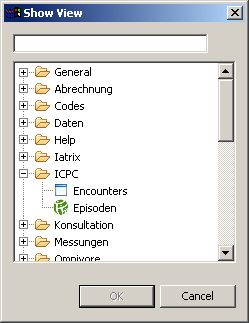
\includegraphics{images/showviewdialog}
  \caption{Liste aller Views}
  \label{fig:viewlist}
\end{center}
\end{figure}

Sie können entweder diese Liste durchblättern, oder Sie können den Namen der
gesuchten View im Textfeld oben eintippen. Sobald Sie anfangen zu tippen, wird
die Liste sofort auf die zu den getippten Buchstaben passenden Einträge
gefiltert.

Markieren Sie dann die gewünschte View und öffnen Sie sie entweder durch
Doppelklick oder Klick auf \glqq OK\grqq{}.

\par
Um eine View zu schliessen genügt es, auf das  X- Symbol im Karteireiter der
betreffenden View zu klicken.

\subsection{Öffnen und Speichern einer Perspektive}
\label{perspektiven} \index{Perspektive}
Eine Perspektive ist wie oben gesagt eine benannte Zusammenstellung von Views.
Elexis bringt einige vordefinierte Perspektiven mit, welche über die Startleiste
resp. die Toolbar aufgerufen werden können. (Vgl auch Abb. \ref{fig:toolbar}).

Eine Perspektive hat als \glqq Startperspektive\grqq{} eine spezielle Bedeutung:
Diese Perspektive wird immer automatisch nach dem Einloggen des entsprechenden
Anwenders auf dem betreffenden Arbeitsplatz eingestellt, sowie nach Klick auf das
'Home'-Symbol (der Button ganz links auf der Toolbar). Alle anderen (beliebig
viele) Perspektiven können unter einem frei wählbaren Namen abgespeichert und
wieder aufgerufen werden. Perspektiven sind Arbeitsplatz-Spezifisch (Eine auf
einem Arbeitsplatz eingestellte Perspektive steht also nicht automatisch auf
anderen Arbeitsplätzen zur Verfügung)\footnote{Dies muss so sein, da ja auch
nicht auf allen Arbeitsplätzen dieselben Plugins zur Verfügung stehen müssen -
vielleicht muss Ihr Buchhaltungs-Plugin nicht unbedingt auch auf dem Labor-PC
aktiv sein.}.

\begin{itemize}
\index{Perspektive!Startperspektive}
\item Um die aktuell eingestellte View-Anordnung als Startperspektive zu
speichern,
wählen Sie den Menüpunkt \textsc{Fenster -- Perspektive -- als Startperspektive
speichern}.

\item Um die aktuelle Perspektive neu (z.B. mit veränderter Viewanordnung oder
-Grösse) zu speichern, wählen Sie das Menü \textsc{Fenster -- Perspektive --
Speichere Perspektive}.

\item Um die aktuelle View-Anordnung unter einem eigenen Perspektivennamen
zu speichern, wählen Sie das  Menü \textsc{Fenster -- Perspektive -- Speichere Perspektive als\ldots}

\item Um die aktuelle Perspektive wiederherzustellen (falls Ihnen die gemachten
Ver\-än\-de\-run\-gen nicht zusagen, oder falls Sie versehentlich Views geschlossen
haben), wählen Sie \textsc{Fenster -- Perspektive -- Wiederherstellen}

\item Um zur Startperspektive zurückzukehren, klicken Sie auf das Haus-Symbol
ganz links in der Toolbar
\item Um eine früher gespeicherte Perspektive aufzurufen, wählen Sie
\textsc{Fenster -- Perspektive -- Andere} und wählen die gewünschte Perspektive
aus der Liste aus.

\end{itemize}

	% *******************************************************************************
% * Copyright (c) 2007 by Elexis
% * All rights reserved. This document and the accompanying materials
% * are made available under the terms of the Eclipse Public License v1.0
% * which accompanies this distribution, and is available at
% * http://www.eclipse.org/legal/epl-v10.html
% *
% * Contributors:
% *    G. Weirich - initial implementation
% *
% *  $Id: stammdaten.tex 4911 2009-01-05 17:56:39Z rgw_ch $
% *******************************************************************************
% !Mode:: "TeX:UTF-8" (encoding info for WinEdt)

\section{'Views' des données de base}

\subsection{patients}
\index{Liste des patients}
La liste des patients affiche les données saisis des patients mais sert aussi pour la saisie des nouvelles entrées. La liste affiche tous les contacts qui sont marqués comme 'patient'.
\begin{figure}[ht]
	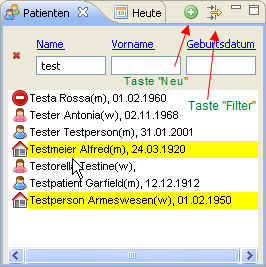
\includegraphics{images/patlistview}
	\caption{Patientenliste}
	\label{fig:patlist}
\end{figure}

Les champs de saisie en haut (nom, prénom, date de naissance) servent à limiter la liste conformément aux paramètres souhaités.
\begin{itemize}
  \item S'applique pour le nom et prénom :
	\begin{itemize}
      \item Si vous suggérez au moins deux lettres, il n'apparaîtront sur la liste que les entrées qui \textit{commencent} avec ces deux lettres.
      \item Lorsque vous introduisez le signe % et au moins deux autres lettres, les entrées qui \textit{contiennent}cette séquence de caractères apparaîtront sur la liste.
    \end{itemize}
  \item S'applique pour la date de naissance :
	\begin{itemize}
      \item Lorsque vous suggérez au moins 3 chiffres successifs les chiffres sont interprétés comme année et les patients qui ont \textit{l'année de naissance } correspondante seront affichés.
      \item Si vous introduisez deux chiffres, suivi d'un point et évtl. d'autres 2 chiffres, les patients avec cette \textit{date de naissance } (jour) et évtuellement \textit{le mois de naissance } correspondant s'afficheront.
      Veuillez considérer que vous devez introduire le jour et le mois toujours à deux chiffres, donc p. ex. 04.05. et non 4.5.
     \end{itemize}
\end{itemize}
S'il n'y a pas de données saisies qui correspondent aux conditions du filtre l'affiche : \glqq pas de données\grqq apparaîtra sur la liste.

\medskip
\index{Patient No} \index{Liste des patients!filtrer}
Vous pouvez influencer les champs des filtres correspondants par un préréglage (cf \ref{userconfig} page \pageref{userconfig}).

\subsubsection{Marquage / Stickers}
\index{patients!marquer}\index{patients!marquer}
Vous pouvez influencer l'affichage de la saisie des patients au moyen de certains critères.
Nous appelons ici cette technique des 'Stickers'. Chaque patient peut avoir zéro à plusieurs 'Stickers' qui peuvent alors apparaître dans la liste des patients aussi bien que dans les notes de la consultation. Vous trouvez des indications plus précises sous  \ref{Etiketten} à la page \pageref{Etiketten};

\subsubsection{Barre d'outils}
\begin{itemize}
  \item Par la touche  \glqq New\grqq{}(bouton vert avec croix blanche)  (cf Fig. \ref{fig:patlist}) vous pouvez saisir un nouveau patient. La boîte de dialogue pour l'introduction des nouveaux patients s'ouvre, si vous cliquez sur ce bouton. Les champs que vous avez déjà remplis y apparaissent et vous pouvez introduire les autres données telles qu'elles sont actuellement connues. En cliquant sur \glqq OK\grqq{}la nouvelle entrée du patient est crée. Si vous cliquez sur\glqq fermer\grqq{}les données sont rejetées et aucune nouvelle entrée est faite. Une demande de précisions apparaîtra si une nouvelle entrée doit être faite lorsqu'une entrée avec les mêmes données existe déjà.



  \item Par la touche  \glqq filtre\grqq{} (cf Fig. \ref{fig:patlist}) vous pouvez ouvrir ou fermer une boite de dialogue pour filtrer la liste selon des différentes critères (cf  Fig. \ref{fig:patlistfilter}).
	\begin{figure}[ht]
        \begin{minipage}{0.5\textwidth}
        \centering
    	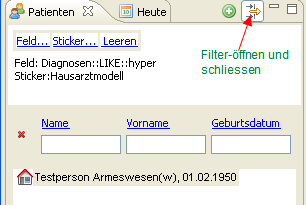
\includegraphics[width=0.8\textwidth]{images/patlistfilter}
    	\caption{Filterbox öffnen}
    	\label{fig:patlistfilter}
        \end{minipage}\hfill
        \begin{minipage}{0.5\textwidth}
        \centering
        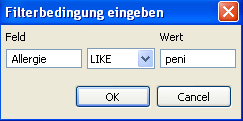
\includegraphics[width=0.8\textwidth]{images/patlistfilter2}
        \caption{Filterausdruck}\label{fig:filterexpr}
        \end{minipage}
    \end{figure}
\end{itemize}

Vous pouvez influencer le filtrage de différentes manières :
\begin{itemize}
\item Si vous cliquez sur 'le champ…' une boîte de dialogue s'ouvre comme dans la Fig. \ref{fig:filterexpr}. Vous pouvez interroger ici des champs de base de données de façon arbitraire. Le '=' signifie : la terminologie doit être exactement la même y inclus l'écriture en majuscule ou minuscule. ' LIKE' signifie : L'expression doit commencer ainsi mais l'écriture en majuscule ou minuscule ne joue aucun rôle.  ' REGEXP signifie: L'expression doit être interprétée comme un terme fixe. Une explication de ce concept conduirait ici toutefois trop loin.


\item Lorsqu'on clique sur 'Sticker' une boite de dialogue s'ouvre qui contient tout les stickers qui sont définis dans le système. Vous pouvez en choisir un ou même plusieurs.
\item Vous pouvez aussi tirer par Drag and Drop un script qui se trouve dans 'script-view' dans le champs de filtrage ce qui permet de calculer des conditions au choix. (cf \ref{Script} à la page \pageref{Script}.
\end{itemize}

Les conditions de filtre sont traitées strictement d'en haut vers le bas. L'expression de filtre
suggérée en deuxième ligne n'est ainsi évaluée que lorsque la première a été passé. Il est donc judicieux d'utiliser des filtres moins intensifs de point de vu calcul (p. ex. Sticker) en haut et ceux qui sont plus intensifs plus bas.(p. ex. Scripts). Cliquez alors sur une des têtes de colonne ou sur 'le x', pour lire la liste -
cette fois-ci sous l'influence des filtres.


\medskip

Pour éliminer une condition de filtre, cliquez la touche droite et choisissez 'éliminer'. Pour éliminer tout, cliquez sur' vider'. Pour mettre le filtre seulement temporairement hors circuit, sans vouloir le vider, cliquez simplement sur le bouton de filtre.


\subsubsection{Menu contextuel}
Le menu contextuel apparaît lorsque vous cliquez avec la touche droite de la souris sur une saisie d'un patient. Il contient les possibilités suivantes :
\begin{itemize}
    \item Sticker … ainsi vous pouvez attribuer un sticker à ce patient ou l'éliminer (cf \ref{Etiketten}).
  \item Effacer le patient (voir ci-dessus)\footnote{pour cela vous nécessitez l'autorisation \textsc{effacer/contact} (cf \ref{sec:gruppen})}
  \item Exporter dossier. Si un Plugin d'exportation est installé ceci permet l'exportation du dossier médical du patient actuellement marqué. Si plusieurs Plugins d'exportation existent il y apparaît une boite de dialogue où on peut choisir la destination et le format\footnote{pour cela vous nécessitez l'autorisation \textsc{fichier/contact/exporter}}
\end{itemize}


\subsection{Patients - détail}
\index{patient!détail}
Cette 'View' (Fig. \ref{fig:patdetail} montre des détails du patient momentanément choisi. 
 %\usepackage{graphics} is needed for \includegraphics

\begin{figure}[t]
\centering
  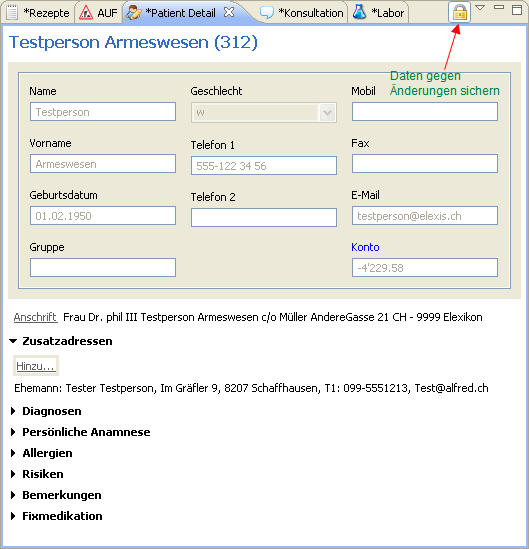
\includegraphics[width=0.8\textwidth]{images/patdetail}
  \caption{Patient Detailansicht}
  \label{fig:patdetail}
  \hfill

\end{figure}

Vous voyez que les différents données saisies apparaissent de couleur grise et ne peuvent pas être modifiées. Si vous cliquez sur le symbole de cadenas à droite en haut, vous pouvez débloquer cette 'View' (si vous possédez les droits correspondants). Ensuite les données de tous les champs peuvent être changées en les écrasant par des nouvelles. Une modification est sauvegardée au moment qu'on quitte un champ. (Le stockage explicite n'est jamais nécessaire dans Elexis). Lorsque vous cliquez de nouveau sur le cadenas ou lorsque vous choisissez un autre patient, la protection se remet en action pour éviter que vous écrasiez des données par erreur.

\medskip

Les champs dans le bloc supérieur sont tous des champs de texte d'une seule ligne et peuvent être modifiés directement à part du champ \glqq compte\grqq{}, qui n'est pas directement réinscriptible. Ce champ affiche le solde de toutes les factures du patient. Si l'utilisateur actuellement inscrit possède les droits d'accéder à la facturation, il peut cliquer sur le texte bleu \glqq compte\grqq{} ce qui ouvre un dialogue dans lequel les différentes payements peuvent être comptabilisés.

\textbf{ATTENTION}: Les écritures se font normalement de façon automatique par la facturation
et l'enregistrement des 'fichiers ESR'. Des écritures manuelles peuvent conduire à des contradictions dans la comptabilité. Ne faites donc des écritures manuelles que lorsque vous êtes conscient des conséquences des changements que vous faites.


 Le champ\glqq adresse\grqq{} indique l'adresse postale du patient.\footnote{L'adresse postale est ce qui apparaît sur les enveloppes et les étiquettes d'adresses. Celle-ci ne doit pas forcément être identique aux données d'adresses introduites. Il peut y apparaître par ex. en plus c/o, cp ou personne de contact} . Celle-ci peut être modifiée en cliquant sur le texte bleu \glqq adresse \grqq{}.

Les champs situé en dessous peuvent tous être ouverts : Normalement seul les titres sont visible et les champs s'ouvrent en cliquant sur le titre.
\begin{itemize}
  \item Le champ \glqq adresses supplémentaires\grqq{}permet de saisir les contacts qui sont en
relation avec un patient. Par exemple membres de famille, offices, d'autres médecins etc. En cliquant sur\glqq ajouter\grqq{} on ouvre une boîte qui contient des différents contacts où on peut choisir ou introduire la personne ou l'organisme en question. Ensuite une autre boîte s'ouvre, dans laquelle les relations du contact choisi avec le patient peuvent être décrites.\\
  Par un clic droit sur une entrée dans ce champ, un menu de contexte s'ouvre qui permet d'afficher out d'éliminer l'entrée entière.
  \item On peut introduire des données dans les champs \glqq Diagnostic\grqq, \glqq Anamnèse personelle\grqq{},
  \glqq Allergies\grqq{}, \glqq Risques\grqq{} und \glqq Remarques\grqq{} lesquelles seront sauvegardées immédiatement lorsqu'on quitte le champ.
  \item Le champ \glqq Médication fixe\grqq{}correspond à la 'View' de la médication fixe.

\end{itemize}
\subsection{Contacts}
Cette 'View' (Fig. \ref{fig:kontaktlist}) montre une liste de tout les contacts introduits dans Elexis. Un contact est chaque personne ou organisation qui a un rapport quelconque avec le cabinet médical. Il s'agit par exemple des patients, collègues, hôpitaux, assurances, laboratoires, fournisseurs etc. 
%\usepackage{graphics} is needed for \includegraphics
\begin{figure}[htp]
\begin{center}
  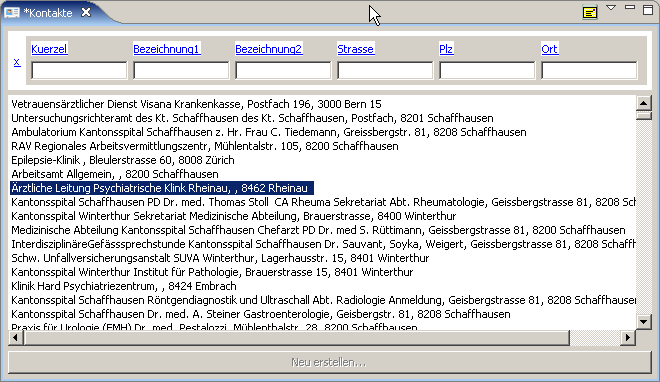
\includegraphics[width=0.9\textwidth]{images/kontaktlistview}
  \caption{Kontaktliste-View}
  \label{fig:kontaktlist}
\end{center}
\end{figure}
En cliquant sur le symbole de l'enveloppe à droite en haut, vous pouvez imprimer une étiquette avec l'adresse du contact choisi.

\subsection{Contacts - détail}
Ici, les détails du contact sélectionné sont indiqués et peuvent être modifiés (Fig. \ref{fig:kontaktdetail}).
%\usepackage{graphics} is needed for \includegraphics
\begin{figure}[htp]
\begin{center}
  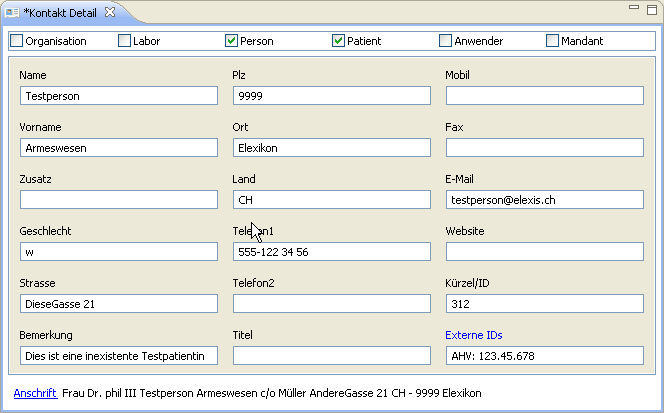
\includegraphics[width=0.9\textwidth]{images/kontaktdetail}
  \caption{Kontakt Detailview}
  \label{fig:kontaktdetail}
\end{center}
\end{figure}
Dans les Checkboxes de la ligne supérieure, vous pouvez définir le type de contact en question. Prenez en considération qu'un contact peut aussi avoir plusieurs types (quelqu'un peut par exemple être utilisateur et également patient ). Par contre un contact ne peut seulement être soit une organisation soit une personne. Veillez également d'introduire ceci correctement. Pour des personnes il ne faut pas oublier de saisir le sexe (m ou f), puisque des modèles de formatage de texte utilisent ces informations pour choisir des formules correctes.

\medskip

Le champ 'sigle/ID' contient sous patients le numéro du patient et ne doit pas être changé. Pour d'autres contacts il peut être utile de définir un sigle spécifique pour pouvoir les trouver plus facilement . Par exemple on peut introduire des médecins avec le préfixe 'méd' suivi de la spécialité et des initiales. Pour les assurances ceci pourrait être le préfix 'ass' etc. L'interniste Docteur Ernst Meier serait à trouver par ex. sous : médIntEM.
L'assurance SWICA à Schaffhouse sous : assSwicaSH.
Les inscriptions ne doivent pas forcément être sans équivoque et on n'est pas forcé d'utiliser ce gadget mais il peut simplement être utile pour rapidement trouver les adresses lorsqu'on doit écrire une lettre.

\medskip

 Le champ'ID externe' sert à établir une quantité arbitraire d'identifications (XID) reçus de l'extérieur. En cliquant sur 'ID externe' de couleur bleue on ouvre un champ de dialogue dans lequel se trouvent toutes les identifications externes déjà existantes. Dans la 'View - contact - détails' on trouve toujours la 'meilleure' càd l'identification la plus sure qui est sans équivoque. Des exemples pour une XID sont le code EAN, le numéro de l'OFSP, des numéros d'assurance sociale/AVS etc.

\medskip

L'adresse postale du contact en question se trouve dans la dernière ligne. Il s'agit de l'adresse, comme elle doit apparaître par exemple dans la zone d'adresse des lettres ou des factures ou sur des étiquettes d'adresse. Cliquez sur le mot en bleu \glqq adresse\grqq{}et la boîte de dialogue d'entrée d'adresse s'ouvre. (Fig.
\ref{fig:anschrift}), où vous pouvez introduire un texte quelconque.  (En cliquant sur le bouton \glqq adresse postale \grqq{} vous créez une adresse standard basée sur les indications des adresses existantes).



\begin{figure}[htp]
\begin{center}
  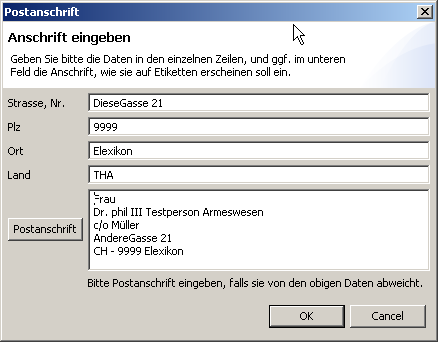
\includegraphics{images/anschrifteingabe}
  \caption{Anschrift-Eingabe}
  \label{fig:anschrift}
\end{center}
\end{figure}
\bigskip
\pagebreak[3]
\subsection{Artikel}
\label{view:artikel}
\index{Article}
Tout objet qui peut être stocké ou / et être remis au patient est un \glqq article\grqq{}. D'un côté ils y existent des articles prédéfinis (par ex. liste de tout les médicaments admis), de l'autre ils y existent aussi des produits propres. Elexis peut administrer le stock des produits et effectuer des commandes de façon semi-automatique pour des articles dont le stock est en train de s'épuiser.


\subsection{Listing des articles}
La Fig. \ref{fig:artikel} montre une liste de sélection d'article et la représentation détaillée des articles.

 %\usepackage{graphics} is needed for \includegraphics
\begin{figure}[htp]
\begin{center}
  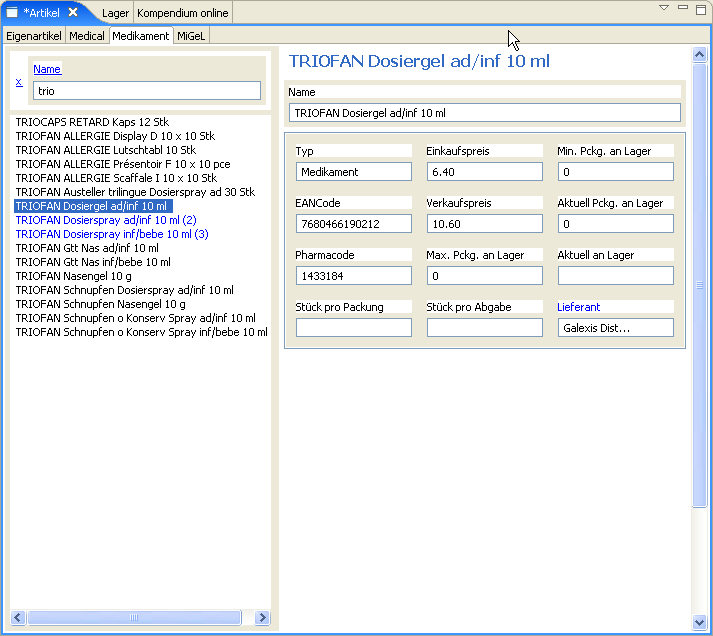
\includegraphics[width=0.9\textwidth]{images/artikelview}
  \caption{Artikel-View}
  \label{fig:artikel}
\end{center}
\end{figure}
Vous pouvez filtrer la liste à gauche de façon habituelle en introduisant les premières lettres du nom de l'article recherché. Vous pouvez voir les détails de l'article sélectionné dans la représentation détaillée. (Dans des perspectives où seulement la liste est représentée, vous pouvez accéder à l'aperçu détaillé en appuyant sur la touche droite de la souris et en choisissant  \glqq modifier\grqq{}.)

\index{Articles}
Un article devient un article en stock lorsque vous lui assignez un inventaire minimal plus grand que zéro. Introduisez en outre un chiffre de stock maximal plus grand que l'inventaire minimal et assignez la valeur correcte au champ \glqq à effectif réel\grqq{}. Elexis fera une commande semi-automatique de chaque article dont l'effectif réel se trouve en dessous de l'inventaire minimal pour pouvoir atteindre le stock maximal.

Certains articles ne sont normalement pas remis par unité d'emballage comme par exemple des ampoules.
Pour cela sont prévus les champs \glqq pièces par emballage\grqq{}et\glqq pièce par remise\grqq{}. Admettons qu'un article est acheté par emballages à 10 pièces mais remis au patients un à un. Dans ce cas vous pouvez introduire sous 'pièce par remise' un 1 et sous 'pièces par emballage' un 10.
Cet article est alors automatiquement comptabilisé au patient comme le 1/10ème du prix de vente par emballage et aussi seulement 1/10ème de l'emballage sera sorti du stock.


La donnée \glqq actuellement en stock\grqq{} veut dire le nombre des articles séparés, tandis que \glqq emballages actuellement en stock\grqq{} indique le nombre des emballages non-ouverts.


\subsection{Stocks et commandes}
\index{commandes!article}
Comme mentionné Elexis est capable d'administrer votre stock de façon semi-automatique. Lorsque vous comptabilisez un article à un patient celui sera automatiquement biffé du stock. Dès que la réserve d'un article en stock tombe sous la limite que vous avez prédéfini, Elexis \glqq se rendra compte \grqq{} qu'il faudra le commander. A part de cette détection automatique vous pouvez naturellement faire ou modifier des commandes de façon manuelle.
Cette fonction se trouve dans la View \glqq Commande grqq{}(cf Fig.\ref{fig:bestellungen}).
 %\usepackage{graphics} is needed for \includegraphics
\begin{figure}[htp]
\begin{center}
  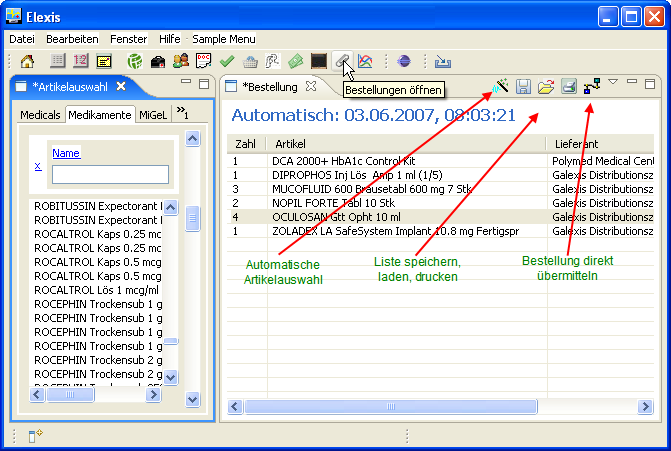
\includegraphics[width=0.9\textwidth]{images/bestell1}
  \caption{Bestellungen - View}
  \label{fig:bestellungen}
\end{center}
\end{figure}


A gauche vous trouvez la fenêtre déjà connue avec la liste de sélection d'article qui contient
toutes les catégories d'articles pour lesquels vous avez des Plugins (normalement pour des médicaments, Medicals, MiGel et des produits propres). 
A droite se trouve le champ pour les commandes qui est d'abord vide. Vous avez donc les possibilités suivantes :

\begin{itemize}
  \item En cliquant sur le symbole de la baguette magique tout les articles dont la quantité est tombée sous la limite de stock prédéfinie par vous seront automatiquement ajoutés à la commande. La commande contiendra autant d'article pour pouvoir atteindre le stock maximal prédéfini pour cet article spécifique.
  \item Depuis la fenêtre gauche vous pouvez aussi tirer un article vers la commande à droite.
	\item En cliquant sur la touche droite de la souris vous pouvez effacer un article de la liste de commande ou changer le chiffre de la quantité commandée.
	\item Vous pouvez sauvegarder d'abord une commande pour l'adapter plus tard. 
	
	\item Vous pouvez recharger des anciennes commandes pour les modifier.
	\item Vous pouvez imprimer les commandes. Pour cela il vous faut un modèle de texte du système (cf page
	\pageref{textvorlagen}) nommée  \glqq commande\grqq{} qui contient à un endroit spécifique un caractère de remplacement  [commande] (cf Fig. \ref{fig:bestell2}).
	\item Last but not least vous pouvez envoyer votre commande par Internet ou modem si vous possédez un Plugin spécifique pour votre livreur. Un Plugin existe déjà pour Galexis et d'autres sont en voie de développement.
\end{itemize}
\begin{figure}[hb]
  % Requires \usepackage{graphicx}
  
\includegraphics{images/bestell2}\\
  \caption{Ausschnitt aus der Vorlage Bestellung}\label{fig:bestell2}
\end{figure}

%\subsection{codes}
%Codes




	% *******************************************************************************
% * Copyright (c) 2007 by Elexis
% * All rights reserved. This document and the accompanying materials
% * are made available under the terms of the Eclipse Public License v1.0
% * which accompanies this distribution, and is available at
% * http://www.eclipse.org/legal/epl-v10.html
% *
% * Contributors:
% *    G. Weirich - initial implementation
% *
% *  $Id: konsviews.tex 4902 2009-01-03 10:47:34Z rgw_ch $
% *******************************************************************************
% !Mode:: "TeX:UTF-8" (encoding info for WinEdt)


\section{Konsultationsbezogene Views}



\subsection{Fälle}
Diese View (Abb. \ref{fig:faelle2} listet alle für den aktuell selektierten
Patienten existierenden Fälle. \index{Fall-Liste}
\begin{wrapfigure}{l}{6.8cm}
  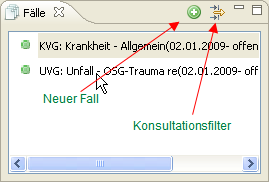
\includegraphics{images/faelleview}
  \caption{Fälle - View}
  \label{fig:faelle2}
\end{wrapfigure}

Das Symbol links von der Fallbezeichnung gibt an, ob alle für die Verrechnung
des Falles notwendigen Daten vorhanden sind: Wenn es grün ist, sollte die
Rechnungserstellung möglich sein, wenn es rot ist, fehlen noch eine oder mehrere
Angaben.

\textit{Welche} Angaben mindestens notwendig sind, hängt vom Abrechnungssystem ab. So ist für Fälle, die nach dem KVG abgerechnet werden, die Angabe
eines Rechnungsempfängers, eines Versicherers und der Versichertennummer
notwendig. Bei Fällen, die nach UVG abgerechnet werden, muss eine Fallnummer
vorhanden sein. Bei Privatrechnungen wird mindestens ein Rechnungsempfänger anzugeben sein.

\medskip

\index{konsultationen!filtern}
\label{filter:fall}
Klick auf das Filtersymbol in der Titelzeile der View führt dazu, dass nu noch diejenigen Konsultationen in der Konsultationsliste (siehe \ref{view:konsultationen}) angezeigt werden, welche zum gerade ausgewählten Fall gehören. Wenn ein anderer Fall angeklickt wird, wird die Liste erneut gefiltert. Erneuter Klick auf das Filter-Symbol schaltet den Filter wieder aus.

Rechtsklick auf einen Fall öffnet dessen Kontextmenü. Dieses enthält die
folgenden Punkte:
\begin{itemize}
  \item {Fall löschen}. Dies ist nur möglich, wenn Sie die dazu notwendigen Rechte
  haben, und wenn zu diesem Fall keine Konsultationen mehr existieren.
  \item {Fall bearbeiten}. Dies öffnet eine weitere View, in der Details zum
  aktuell ausgewählten Fall eingegeben werden können.
  \item {Fall wieder öffnen}. Damit kann man einen bereits
  geschlossenen\footnote{Ein Fall ist dann geschlossen, wenn ein End-Datum
  eingegeben wurde. Zu einem geschlossenen Fall können keine Konsultationen mehr
  hinzugefügt werden.} Fall wieder öffnen.
  \item {Rechnung erstellen}. Hiermit lässt sich über alle unverrechneten
  Konsultationen des aktuellen Falls und des aktuellen Mandanten eine Rechnung
  erstellen. Dies ist eine \glqq Abkürzung\grqq{} des normalen Wegs der
  Rechnungserstellung und eignet sich vor allem für Sofortrechnungen einzelner
  Konsultationen oder Leistungen.
\end{itemize}


\clubpenalty=5000

\subsection{Fälle und Kons}
 %\usepackage{graphics} is needed for \includegraphics
\begin{wrapfigure}{l}{7cm}
  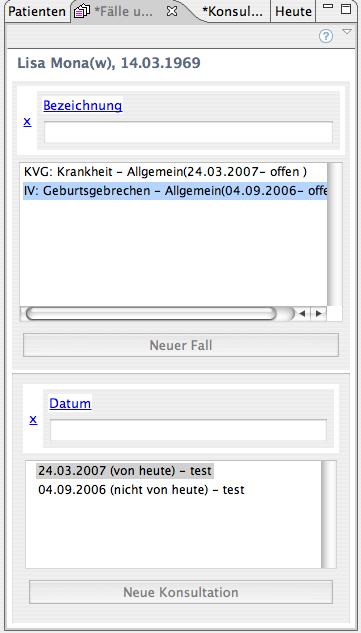
\includegraphics[width=7cm]{images/fallkonsview}
  \caption{Fälle und Kons}
  \label{fig:fallkons}
\end{wrapfigure}
Diese View (Abb. \ref{fig:fallkons} listet synoptisch Fälle und dazugehörige
Konsultationen (Nur Titel ohne Texte) auf. Wenn im oberen Bereich ein Fall
angeklickt wird, werden im unteren Bereich die zu diesem Fall gehörenden
Konsultationen angezeigt. Wenn eine Konsultation angeklickt wird, wird diese
Konsultation in der Konsultation-View (S. \ref{konsview} s. \pageref{konsview}) angezeigt.

Um einen neuen Fall zu erstellen, geben Sie einen Titel für diesen Fall ein und klicken dann auf \textit{neuer Fall}. Um eine neue Konsultation einzugeben, wählen Sie den dazugehörigen Fall aus und klicken auf \textit{Neue Konsultation}

\medskip

Anmerkung: Sie werden festgestellt haben, dass diese View und die vorher besprochene Fälle-View bis zu einem gewissen Punkt redundant sind. Das ist auch so. Sie können getrennte Views für Fälle und Konsultationen bevorzugen, oder eine View in der beides enthalten ist. In der Regel werden Sie nicht beide Konzepte anwenden, sondern dasjenige, welches Ihnen besser gefällt - Elexis lässt Ihnen die Wahl.

\clearpage

\subsection{Konsultationen}
\label{view:konsultationen}
\begin{wrapfigure}{L}{7.5cm}
  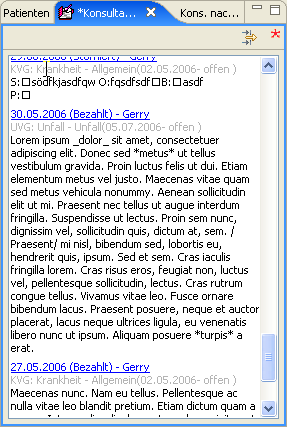
\includegraphics{images/konslisteview}
  \caption{Konsultationsliste}
  \label{fig:konslisteview}
\end{wrapfigure}

Dies ist eine Auflistung aller bisherigen Konsultationen des aktuell
selektierten Patienten, unabhängig vom jeweiligen Fall.
\index{Konsultationsliste} Zu jeder Konsultation
wird der Text ohne Formatierungen angezeigt. (S. Abb. \ref{fig:konslisteview}).\\
Klick auf den (blauen) Titel einer Konsultation wählt diese Konsultation in der
Konsultation-View (s. S. \pageref{konsview}) aus.

Klick auf das Filter-Symbol rechts oben öffnet den Filter-Dialog (s. Abb. \ref{fig:konsfilter}).
\index{Konsultationsfilter} Hier können Sie bestimmte Kriterien eingeben, nach
denen die angezeigten Konsultationen gefiltert werden sollen (d.h. es werden nur
noch diejenigen Konsultationen angezeigt, die den Filterbedingungen
entsprechen).

Im oberen Feld können Sie angeben, ob nur Konsultationen eines bestimmten Falls
oder aller Fälle angezeigt werden sollen. Im unteren Feld können Sie
Suchbegriffe eingeben, welche im Konsultationstext vorkommen müssen. Mehrere
Suchbegriffe können mit AND, OR, NOT, AND NOT und OR NOT miteinander verknüpft werden.
Beispielsweise findet \glqq Lorem AND NOT ipsum\grqq{} nur solche Konsultationen, deren
Text \glqq Lorem\grqq, nicht aber \glqq ipsum\grqq{}enthält.

Ganz unten können Sie schliesslich noch angeben, ob Gross/Kleinschreibung
beachtet werden soll, oder ob Suchbegriffe als reguläre Ausdrücke betrachtet
werden sollen. Eine genaue Erklärung dieses Themas würde hier zu weit führen;
Sie finden sehr viel Literatur dazu mit den Stichwörtern \glqq Regular
Expression\grqq{}oder \glqq Pattern Matching\grqq{}. Diese Technik erlaubt es,
den Suchbegriff mit verschiedensten Platzhaltern zu beschreiben. So würde z.B.
\glqq M[ae][iy]e?r\grqq{} nach allen Meiers, Mayrs etc. in allen Schreibweisen
suchen.

\medskip

Anmerkung:
Das Filtern der Konsultationen mit diesem Verfahren kann, da der Text jeder Konsultstion komplett durchsucht wird, einige Sekunden dauern. Wenn man lediglich nach Fällen oder Problemen filtern möchte, ist der entsprechende Fallfilter (S. \pageref{filter:fall}) oder Problemliste-Filter (S. \pageref{filter:problemliste})im Allgemeinen effizienter.

\begin{figure}[ht]
\begin{center}
  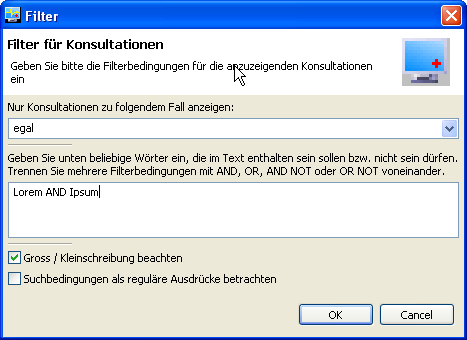
\includegraphics{images/filterdialog}
  \caption{Filterdialog}
  \label{fig:konsfilter}
\end{center}
\end{figure}


\subsection{Konsultation}
 \label{konsview}
Detailansicht eines Konsultationseintrags (S. Abb. \ref{fig:konsdetail}).
\begin{figure}[ht]
  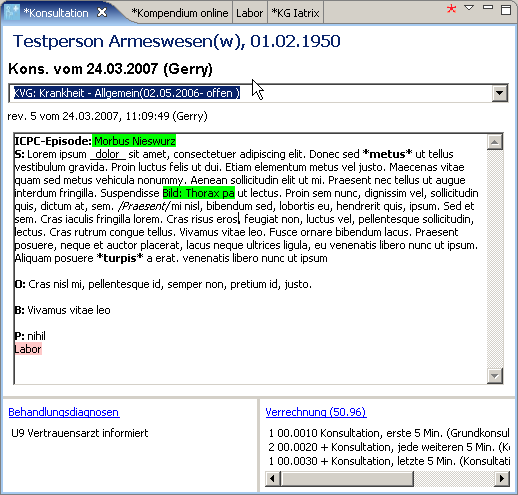
\includegraphics{images/konsview}
  \caption{Konsultation: Detail}
  \label{fig:konsdetail}
\end{figure}

Sie haben im Textfeld folgende zusätzlichen Möglichkeiten:
\begin{description}
\item[Makros]
Schreiben Sie einen beliebigen Text, markieren Sie diesen Text mit der linken Maustaste, klicken Sie dann mit der rechten Maustaste und wählen Sie "'als Makro..."'. eben Sie dem Makro einen beliebigen Namen. Wenn Sie nun zukünftig den Namen des Makros gefolgt von \# tippen, wird dieser Text durch den vorher definierten Inhalt des Makros ersetzt.

\item[Abrechnen]
Wenn Sie den Namen eines Abrechnungsblocks tippen, gefolgt von \#, dann wird dieser Block verrechnet, ebenso, wie wenn Sie ihn mit der Maus ins Verrechnungs-Feld gezogen hätten.

\item[Textauszeichnungen]
Es können auch einige einfache Textauszeichnungen gemacht werden: Ein Wort am Anfang einer Zeile, welches von einem Doppelpunkt gefolgt ist, wird fett gedruckt. Ebenso ein Wort zwischen zwei *. Ein Wort zwischen zwei / wird kursiv geschrieben.
\end{description}


\subsection{AUF}
Diese View dient der Festlegung einer Arbeitsunfähigkeit. (Abb \ref{fig:auf})
\index{AUF} \index{Arbeitsunfähigkeit}.
\begin{figure}
  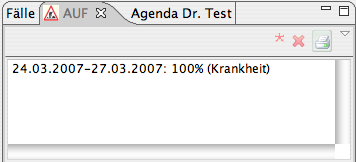
\includegraphics{images/aufview}
  \caption{AUF-View}
  \label{fig:auf}
\end{figure}
Eine AUF bezieht sich immer auf einen bestimmten Fall. Wenn kein Fall markiert
ist, werden Sie aufgefordert, zunächst einen anzugeben.

Wenn Sie auf das \glqq Neu\grqq -Symbol (roter Stern) klicken, erscheint ein
Dialog, in dem Sie Anfang und Ende der neuen Arbeitsunfähigkeit festlegen
können. Klick auf das \glqq Drucker\grqq -Symbol öffnet eine Text-View, in der
Sie noch manuelle Änderungen am AUF-Text ergänzen können, bevor Sie das Zeugnis
definitiv ausdrucken oder aufs Fax senden.

\subsection{Rezepte}
In dieser View werden Rezepte aufgenommen. \index{Rezept}Klicken Sie auf das \glqq Neu\grqq
-Symbol (grünes plus) und es wird ein neues Rezept mit dem Aktuellen Datum
erstellt. Ziehen Sie Artikel mittels Drag\&Drop aus einer Artikelliste oder der
Dauermedikations-View in dieses Rezept. Mit Klick auf das \glqq Drucker\grqq -
Symbol öffnen Sie eine Text-View, in der Sie noch manuelle Änderungen anbringen
können, bevor Sie das Rezept definitiv auf den Drucker oder ein Faxgerät oder in
einen Export-Konnektor senden.
Hierzu muss eine Textvorlage namens \glqq Rezept\grqq
existieren, welche an einer Stelle den Platzhalter [Rezeptzeilen] enthält. Dort
werden die ausgewählten Artikel eingefügt.


\subsection{Falldetail}
\label{falldetail}
\index{Fall!Detailansicht}
Diese View (Abb. \ref{fig:falldetail}) dient zum Einstellen der Details eines Falls (Eine Dialogbox mit derselben View wird geöffnet, wenn man einen neuen Fall (s. \ref{definition:fall} S. \pageref{definition:fall}) erstellt).
\begin{figure}[ht]
  % Requires \usepackage{graphicx}
  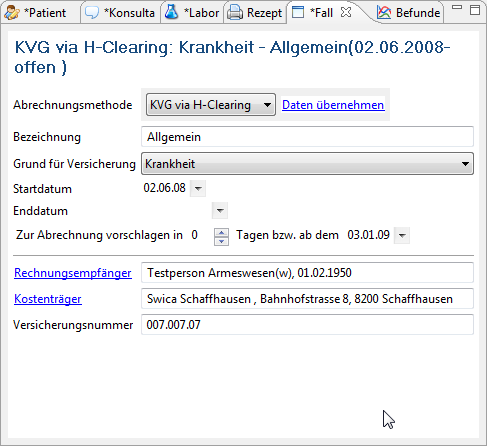
\includegraphics[width=0.8\textwidth]{images/falldetail}\\
  \caption{Fall-Detail}\label{fig:falldetail}
\end{figure}
In der obersten Auswahlbox geben Sie an, welches Abrechnungssystem (S. auch \ref{settings:abrechnungssystem} auf Seite \pageref{settings:abrechnungssystem}) für diesen Fall angewendet werden soll. Darunter steht eine Bezeichnung für den fall, die Sie frei wählen können. Diese dient nur Ihrer eigenen Information, damit Sie verschiedene Fälle desselben Patienten einfacher auseinanderhalten können. Die nächste Zeile, 'Grund für die Versicherung' ist eine Angabe, die auf den zu diesem fall erstellten Rechnungen stehen wird (Falls die Rechnungsvorlage ein entsprechendes Feld enthält).

Das \textbf{Startdatum} ist üblicherweise das Datum der ersten Konsultation, oder bei Unfällen, das Unfalldatum. Das \textbf{Enddatum} hingegen bezeichnet das Datum, wen der Fall abgeschlossen wird. Ein Fall, welcher ein Enddatum hat, wird in der Fall-Liste (Abb. \ref{fig:faelle2}) als 'GESCHLOSSEN' markiert. Zu einem solchen Fall können keine Konsultationen mehr erstellt werden.
In der Regel sollte ein Fall nur abgeschlossen werden, wenn es ein Unfall ist, welcher abgeschlossen ist, oder wenn der Patient den Versicherer wechselt und die Abrechnungsdaten darum ändern.

Die nächste Zeile, Rechnungsempfänger, ist zwingend, damit überhaupt eine Rechnung erstellt werden kann. Dies muss ein bereits existierender Kontakt (z.B. der Patient selbst) sein.

\medskip
Alle weiteren Zeilen sind je nach gewähltem Abrechnungssystem unterschiedlich. Oft wird auch eine Zeile 'Kostenträger' vorhanden sein \footnote{Wichtige Anmerkung für das \textbf{Tarmed-System} (Schweiz): Wenn Rechnungsempfänger und Kostenträger identisch sind, wird eine Tiers Payant-Rechnung erstellt, andernfalls eine Tiers-Garant-Rechnung. Achten Sie also darauf, dass diese beiden Zeilen korrekt sind (Bei UVG-Fällen müssen also sowohl Rechnungsempfänger als auch Kostenträger der jeweilige Unfallversicherer sein, während bei KVG-Fällen in TG-Kantonen der Patient der Rechnungsempfänger und die Krankenkasse der Kostenträger ist)}.

\clearpage

\subsection{Diagnosen}
\label{view:diagnosen} \index{Diagnosen}
Diese View (Abb. \ref{fig:diagnosen}) dient dazu, Diagnosen auszuwählen und einer Konsultation zuzuordnen.
 \begin{wrapfigure}{l}{7cm}
    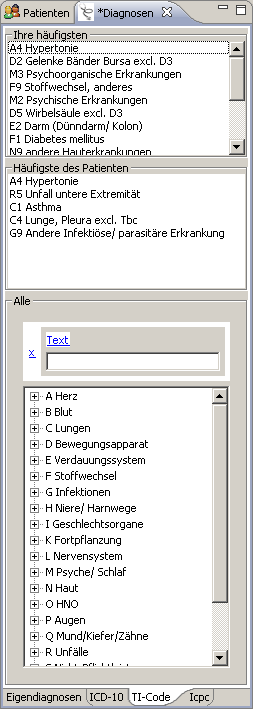
\includegraphics[width=6.5cm]{images/diagnosenview}
    \label{fig:diagnosen}
    \caption{Diagnosen-Auswahl}
\end{wrapfigure}
Unten sehen Sie eine Reihe von Reitern, die den installierten Diagnosecode-Plugins entsprechen (standardmässig TI-Code, ICD-10, und ICPC-2).
Um eine Diagnose auszuwählen, wählen Sie zunächst aus diesen Reitern das entsprechende Codesystem und dann den Code. Die Auswahl kann durch Drag\&Drop oder durch Doppelklick erfolgen.
Für jedes Codesystem sehen Sie ein dreigeteiltes Fenster: Im obersten Bereich sind Ihre (d.h. des aktuell eingeloggten Anwenders) am häufigsten eingesetzten Diagnosen zu sehen; im mittleren Teil diejenigen Diagnosen, die beim aktuell ausgewählten Patienten bisher am häufigsten verwendet worden sind, und um unteren Teil die gesamte Systematik des gewählten Codesystems.

\medskip

Auf diese Weise haben Sie stets Zugriff auf die am häufigsten benötigten Codes und werden nur noch selten die ganze Systematik durchsuchen müssen.


	% *******************************************************************************
% * Copyright (c) 2007 by Elexis
% * All rights reserved. This document and the accompanying materials
% * are made available under the terms of the Eclipse Public License v1.0
% * which accompanies this distribution, and is available at
% * http://www.eclipse.org/legal/epl-v10.html
% *
% * Contributors:
% *    G. Weirich - initial implementation
% *
% *  $Id: laborview.tex 4902 2009-01-03 10:47:34Z rgw_ch $
% *******************************************************************************
% !Mode:: "TeX:UTF-8" (encoding info for WinEdt)

\section{Laboranzeige-View}
\index{Labor!Eingabe}
\index{Labor!Anzeige}
Bei Elexis werden sowohl interne als auch externe Laborbefunde, sowohl
automatisch eingelesene als auch manuell eigegebene Befunde in derselben Sicht
angezeigt.

Die  Anzeige eines Befundes wird bestimmt durch
\begin{itemize}
  \item Ein Laboritem, zu dem dieser Befund gehört
  \item Ein Datum, an dem dieser Befund erhoben wurde
  \item Einen Patienten, zu dem dieser Befund gehört
\end{itemize}

Das Laboritem definiert, wie und wo der Laborbefund angezeigt werden soll, und
zu welchem Typ von Laborwerten er gehört. Das Erstellen von Labritems ist in der Regel nur bei der Installation des
Programms notwendig, bzw. dann, wenn Sie neue Laborparameter in Ihre
Standardbesimmungen aufnehmen möchten. Das genaue Vorgehen ist unter Konfiguration (S. \pageref{config:labor} genauer beschrieben.

 %\usepackage{graphics} is needed for \includegraphics
\begin{figure}[htp]
\begin{center}
  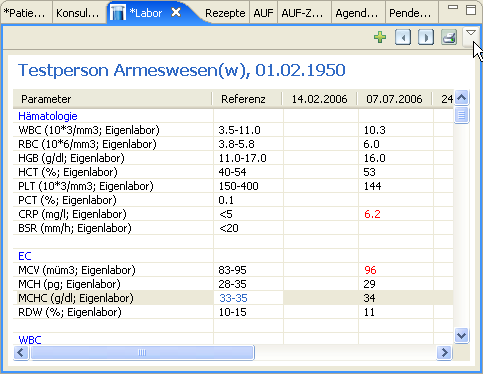
\includegraphics{images/labview}
  \caption{Labor-Anzeige}
  \label{fig:labview}
\end{center}
\end{figure}

\subsection{Manuelle Eingabe}
Um Laborwerte manuell einzutragen, gehen Sie so vor:
\begin{itemize}
    \item Wenn für das gewünschte Datum noch keine Spalte exstiert, klicken Sie auf das grüne Pluszeichen rechts oben, um ein Datum anzugeben.
    \item klicken Sie auf die Zeile und Spalte, wo Sie einen Laborwert eingeben möchten. Tippen Sie den Wert ein und verlassen Sie das Feld mit der Eingabetaste, oder der Pfeil-nach-unten-Taste.
\end{itemize}
Wenn ein Laborparameter numerisch ist, und der eingegebene Wert ausserhalb des Referenzbereichs ist, wird der Wert in rot angezeigt. Sie können diese Anzeige auch manuell ein- und ausschalten, indem Sie den Wert mit der rechten Maustaste anklicken und das Häkchen vor \glqq pathologisch\grqq{} setzen oder löschen.

\subsection{Automatisches Einlesen}
\index{Labor!automatisches Einlesen}
Elexis kann Laborwerte selbstverständlich auch automatisch einlesen. Hierfür dient das View-Menu rechts oben:\\
\begin{wrapfigure}{r}{7cm}
    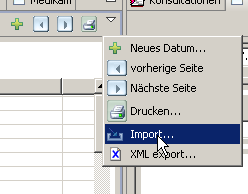
\includegraphics{images/labor6}
\end{wrapfigure}
Klicken Sie auf \textit{import} und wählen Sie in der dann erscheinenden Dialogbox die Quelle für die einzulesenden Laborwerte aus. Was für Quellen hier angeboten werden, hängt von den vorhandenen Laborimport-Plugins ab. In Frage kommen Laborgeräte und verschiedene externe Labors. Eine aktuelle Liste aller vorhandenen Laborimport-Plugins finden Sie auf http://www.elexis.ch

\subsection{Laborblatt drucken}
Um ein Laborblatt auszudrucken, klicken Sie auf das Drucker-Symbol rechts oben. Dies erstellt eine Tabelle innerhalb einer System-Textvorlage \glqq Laborblatt\grqq{}, welche einen Platzhalter [Laborwerte] enthalten muss (s. auch \ref{textvorlagen}).

\section{Labor Neu}
Diese View dient dazu, alle Laborwerte anzuzeigen, welche noch nicht als \glqq gesehen\grqq{} markiert worden sind, und erlaubt es auch gleich, sie als gesehen zu markieren (S. Abb. \ref{fig:labneu}).

\begin{figure}
  % Requires \usepackage{graphicx}
  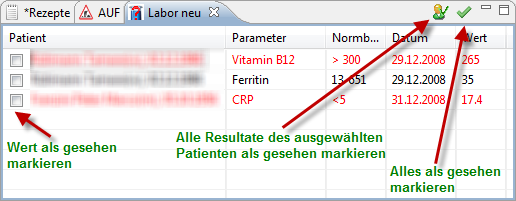
\includegraphics{images/labneu1}\\
  \caption{Anzeige neuer Laborwerte}\label{fig:labneu}
\end{figure}

Werte ausserhalb des Referenzbereichs werden rot dargestellt. Man kann gesehene Werte mit einem Häkchen in der Checkbox links markieren. Nach einiger Zeit werden diese dann aus der Liste entfernt (Solange sie noch nicht entfernt sind, kann man die Markierung mit einem erneuten Klick wieder löschen). Werte die älter als 96 Stunden sind, werden automatisch aus der Liste entfernt.

Wenn man einen Eintrag markiert wird das Laborblatt des betreffenden Patienten aktiviert (sofern eine Labor-View geöffnet ist). Man kann entweder einen einzelnen Wert oder alle Resultate des aktuell markierten Patienten, oder alle angezeigten Resultate als gelesen markieren.

Um die Werte einzeln oder gesamthaft als gesehen zu markieren, ist das Recht \textit{Daten/Patient/Labor abhaken} erforderlich (s. \ref{sec:gruppen}, S. \pageref{sec:gruppen}ff.)

	% *******************************************************************************
% * Copyright (c) 2007 by Elexis
% * All rights reserved. This document and the accompanying materials
% * are made available under the terms of the Eclipse Public License v1.0
% * which accompanies this distribution, and is available at
% * http://www.eclipse.org/legal/epl-v10.html
% *
% *  $Id: abrechnung.tex 4911 2009-01-05 17:56:39Z rgw_ch $
%
%*******************************************************************************
% !Mode:: "TeX:UTF-8" (encoding info for WinEdt)

\section{Abrechnungsbezogene Views}
\subsection{Konsultationen nach Datum}
\begin{wrapfigure}{l}{7.3cm}
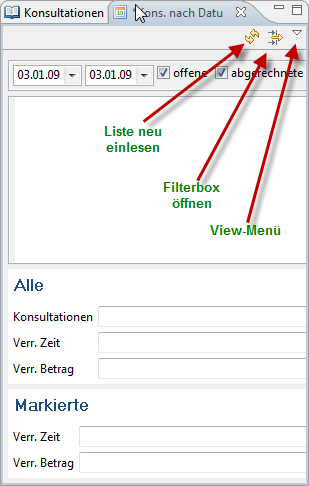
\includegraphics[width=7cm]{images/heute}
\caption{Konsultation nach Datum}
\label{fig:heute}
\end{wrapfigure}

Diese View (Abb. \ref{fig:heute}) dient dazu, Konsultationen eines bestimmten Zeitraums (standardmässig
des aktuellen Tages) darzustellen. Sie gibt einen Überblick über Verrechnung und
verrechnete Zeit jeder Konsultation einzeln und der Summe davon. Durch Anklicken der entsprechenden Checkbox können Sie angeben, ob offene\footnote{also solche, von denen bisher keine Rechnung erstellt wurde} oder abgerechnete Konsultationen (oder beides) gezählt werden sollen. In den Datumsfeldern können Sie Start- und Enddatum des gewünschten Zeitraums angeben. Nach jeder Änderung müssen Sie auf den 'Neu einlesen'-Knopf klicken, damit die Liste neu gezählt wird.

\medskip

Im unteren Abschnitt der View sehen Sie die Gesamtzahl der Konsultationen im
gewählten Zeitraum, sowie die (vom Abrechnungssystem her vorgegebene)
verrechnete Zeit und den verrechneten Betrag. Im Feld darunter sehen Sie
dieselben Angaben für die aktuell markierte Konsultation.

Sie können diese View also auch verwenden, um Abends kurz die Konsultationen des Tages
durchzugehen um unverrechnete oder falsch verrechnete zu korrigieren.

\medskip

Ausserdem erlaubt diese View einfache statistische Funktionen:
%\begin{itemize}
Wenn Sie die Taste 'Filter' klicken, öffnet sich im oberen Teil der View eine Filterbox. Sie können aus einem Verrechnungsfenster diejenigen Positionen in diese Box ziehen, die Sie zählen wollen. Beim nächsten Einlesen zählt die View dann nur noch solche Konsultationen, bei denen einer der gewünschten Codes verrechnet wurde und listet dann (beim Ausdrucken, s. weiter unten), die Codes und Gesamtbeträge separat auf.

\medskip

 Im View-Menü finden Sie die Option 'Liste drucken'. Dadurch öffnet sich ein Fenster mit einer Tabelle, welche die angezeigten Konsultationen auflistet und ausdrucken lässt.

\medskip

 Für detailliertere Statistiken können Sie ebenfalls im View-Menü die Option 'Statistik' auswählen. Dies liefert eine Datei im CSV\footnote{Character Separated Values; ein Standard-Format für tabellarische Daten}- Format, die mit anderen Programmen wie OpenOffice.org calc oder Microsoft\texttrademark Excel\texttrademark eingelesen und statistisch aufbereitet werden kann. Diese Datei enthält alle abgerechneten Positionen mit Häufigkeit, Kosten und Umsatz.


\subsection{Konsultationen zum Verrechnen}
\index{Abrechnung} Diese View (s. fig. \ref{fig:konsv}) dient dazu, diejenigen
Konsultationen
auszuwählen, von welchen eine Rechnung erstellt werden soll. Es werden dabei nur
die Konsultationen des aktuellen Mandanten angezeigt.
\begin{figure}[hb]
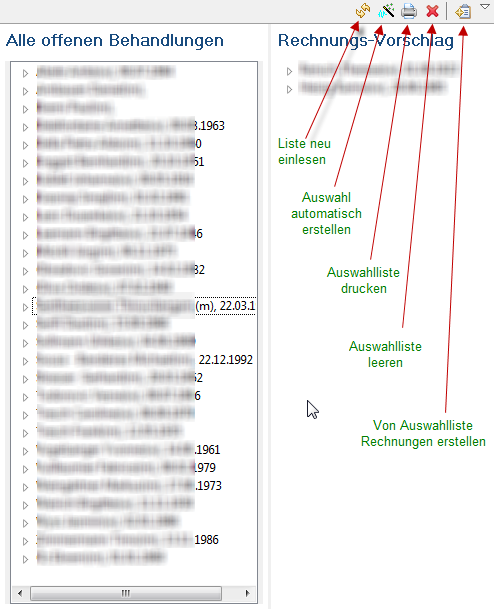
\includegraphics{images/konsv}
\caption{Konsultation zur Verrechnung auswählen}
\label {fig:konsv}
\end{figure}
Hierzu gibt es folgende Möglichkeiten:
\begin{itemize}
  \item Automatische Auswahl (Zauberstab-Icon): Dabei werden die Konsultationen nach bestimmten Regeln automatisch ausgewählt und in die Auswahlliste
  übertragen. Dies wird weiter unten (Rechnungsautomatik) genauer ausgeführt.
  \item Patientennamen aus der Liste in die Auswahl ziehen: Dadurch werden alle
  Konsultationen aller Fälle des gewählten Patienten zur Abrechnung markiert.
  \item Fälle aus der Liste in die Auswahl ziehen: Dadurch werden alle
  Konsultationen der gewählten Fälle zur Abrechnung markiert.
  \item Konsultationen aus der Liste in die Auswahl ziehen: Dadurch werden nur
  die gewählten Konsultationen zur Abrechnung vorgemerkt.
\end{itemize}
Bei allen Methoden können Sie die Auswahl nachträglich noch beliebig ändern. Sie
können weitere Elemente zufügen, oder Sie können (nach Rechtsklick auf ein
Element in der Auswahl) Elemente entfernen, oder Sie können die ganze Auswahl
wieder löschen. Zu diesem Zeitpunkt sind noch keinerlei Änderungen der Daten
erfolgt.

Wenn Sie die Auswahl fertig erstellt haben, können Sie auf \glqq Rechnungen
erstellen\grqq klicken, dann werden Rechnungen für alle in der Auswahl
befindlichen Elemente erstellt. Dabei werden immer alle Konsultationen, die zu
einem Fall gehören, zusammengefasst. Wenn von einem Patienten also mehrere Fälle
in der Auswahl sind, werden auch mehrere Rechnungen erstellt.

\subsubsection{Rechnungsautomatk}
\index{Rechnungsautomatik}\label{auto}
Hiermit werden Konsultationen nach bestimmten wählbaren Kriterien zum Abrechnen vorgeschlagen (S. Abb. \ref{fig:rnautomatik}).
\begin{figure}
  % Requires \usepackage{graphicx}
  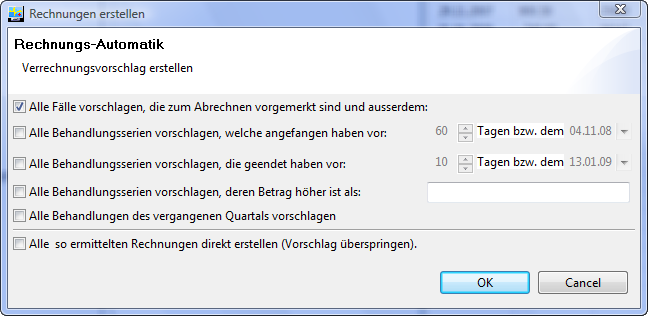
\includegraphics[width=1.0\textwidth]{images/rechnungsautomatik}\\
  \caption{Halbautomatischer Rechnungsvorschlag}\label{fig:rnautomatik}
\end{figure}

\begin{itemize}
\item Alle Fälle vorschlagen, die zum Abrechnen vorgemerkt sind: Wenn Sie diese Checkbox anklicken werden die Konsultationen jener Fälle ausgewählt, bei denen Sie ein Abrechnungsdatum im Fall-Detail spezifiziert hatten (Vgl. Abb. \ref{fig:falldetail}).
\item Alle Behandlungsserien vorschlagen, welche angefangen haben vor...: Damit werden sämtliche unverrechneten Konsultationen eines Falls (bis heute) ausgewählt, sofern mindestens eine der Konsulationen vor dem Stichtag stattgefunden hat.
\item Alle Behandlungsserien vorschlagen, die geendet haben vor...: Damit werden sämtliche unverrechneten Konsultationen eine Falls ausgewählt, sofern die letzte Konsultation vor dem Stichtag stattgefunden hat.
\item Alle Behandlungsserien vorschlagen, deren Betrag höher ist als...: Alle unverrechneten Konsultationen eines Falls werden ausgewählt, sofern deren Gesamtbetrag höher als der genannte Grenzwert ist.
\item Alle Behandlungen des vergangenen Quartals vorschlagen: Hierbei wird das letzte \textit{Kalenderquartal} abgerechnet. Es gelten also die Stichtage 31.3., 30.6, 30.9. und 31.12.
\end{itemize}
Bei allen Optionen gilt, dass sie nur ausgewertet werden, wenn das Häkchen in der Checkbox gesetzt ist. Es genügt also nicht, einen Wert einzutragen. Die verschiedenen Optionen gelten additiv: Es wird also am Schluss jede Konsultation ausgewählt, für die mindestens eine der aktiven Kriterien zutrifft.

\medskip

\clearpage

\subsection{Rechnungen}
\begin{figure}[ht]
  % Requires \usepackage{graphicx}
  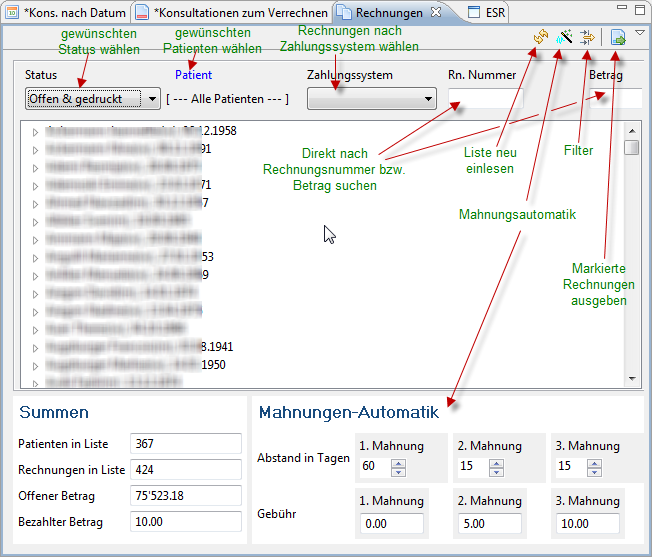
\includegraphics[width=1.0\textwidth]{images/rechnungsview}\\
  \caption{Rechnungen-View}\label{fig:rechnungen}
\end{figure}

In dieser View (Abb. \ref{fig:rechnungen}) sehen Sie die erstellten Rechnungen. Eine Rechnung hat immer einen bestimmten Status:
\begin{description}
    \item [Offen] Unmittelbar nach dem Erstellen.
    \item [Offen und gedruckt] Die Rechnung wurde mindestens einmal ausgegeben (über den Drucker oder eine andere Exportmethode). Ab diesem Zeitpunkt beginnt die Zahlungsfrist zu laufen. (Elexis kann allerdings nicht feststellen, ob beispielsweise der Drucker die Rechnung nicht korrekt ausgedruckt hat, oder ob sie nicht abgeschickt wurde. Deshalb liegt in diesem Punkt eine potentielle Fehlerquelle)
    \item[Zahlungserinnerung] Die Zahlungserinnerung wurde erstellt, aber noch nicht ausgedruckt
    \item[ZE gedruckt] Die Zahlungserinnerung wurdr ausgedruckt
    \item [2. Mahnung erstellt, 2. Mahnung gedruckt, 3. Mahnung erstellt, 3. Mahnung gedruckt]: analog
    \item[Teilweise bezahlt] Es ist (mindestens) eine Zahlung eingebucht, welche aber nicht den ganzen Rechnungsbetrag abdeckt.
    \item[bezahlt] Der Rechnungsbetrag wurde (in einer oder mehreren Buchungen) vollständig bezahlt
    \item [zuviel bezahlt] Auch das kommt vor.
    \item [Teilverlust] Ein Teil des Rechnungsbetrages wird abgeschrieben (Im Gegensatz zu \glqq Teilweise bezahlt\grqq{} rechnen Sie hier nicht mehr mit einer weiteren Zahlung)
    \item [Totalverlust] Der Rechnungsbetrag wird komplett abgeschrieben
    \item [In Betreibung] Genau das.
    \item [Storniert] Eine einmal erstellte Rechnung kann nicht mehr gelöscht werden. Das muss so sein, weil sonst die Situation möglich wäre, dass jemand eine nicht mehr existierende Rechnung reklamiert, oder dass Rückfragen zu einer inexistenten Rechnung kämen. Wenn eine Rechnung aus irgendeinem Grund ungültig ist (Fehler, Erlassen des Betrags etc.), dann muss sie stattdessen storniert werden. Stornieren hat in allen praktischen Belangen denselben Effekt wie löschen, ausser, dass die Rechnungsnummer vergeben bleibt und dass die Rechnung später wieder betrachtet werden kann.
    \item [fehlerhaft] Wenn ein Rechnungsausgabemodul feststellt, dass eine Rechnung fehlerhaft ist (beispielsweise könnte das TrustX-Modul monieren, dass nicht alle EAN-Nummern angegeben sind), dann erhält die betreffende Rechnung den Status fehlerhaft und kann so korrigiert werden.
    \item [zu drucken] Diese Einstellung findet alle Rechnungen, die offen, aber noch nicht gedruckt sind (also auch ungedruckte Mahnungen etc.)
    \item [ausstehend] Zusammenfassung aller 'offen und gedruckt', 'ZE gedruckt', '2.Mahnung gedruckt', '3. Mahnung gedruckt', 'Teilweise bezahlt' und 'In Betreibung'. Also alle Rechnungen, von denen noch Zahlungen erwartet werden.
    \item [Mahnstopp] Genau das.
\end{description}

Die Rechnungsliste kann nach bestimmten Kriterien selektiert werden. Um die Liste mit den geänderten Optionen neu einzulesen, klicken Sie jeweils auf den 'Liste neu einlesen'-Knopf.
Um die Rechnungen mit einem bestimmten Status anzuzeigen, wählen Sie diesen Status in der Combox links oben aus(S. Abb. \ref{fig:rechnungen}). Um nur die Rechnungen eines bestimmten Patienten anzuzeigen, klicken Sie auf die blaue Schrift \glqq Patient\grqq{}. Es öffnet sich die bekannte Kontaktauswahl-Dialogbox. Wählen Sie dort einen Patienten aus und klicken Sie ok, oder klicken Sie auf Abbrechen, um wieder alle Patienten anzuzeigen.

Um nur eine bestimmte Rechnungsnummer auszuwählen, geben Sie diese Nummer im Feld Rn-Nummer ein und drücken die Eingabetaste oder klicken 'neu einlesen'. Um Rechnungen mit einem bestimmten Betrag zu suchen (z.B. um eine unklare Zahlung zuzuordnen), geben Sie den Betrag ein und drücken die Eingabetaste.

\medskip
Wenn Sie auf das 'Filter'-Symbol klicken, erhalten Sie weitere Darstellungsoptionen.

\begin{wrapfigure}{l}{7cm}
\includegraphics[width=7cm]{images/rechnungsfilter}
\end{wrapfigure}
Die Felder Betrag von/bis dienen dazu, Rechnungen mit einem bestimmten Betrag auszufiltern. Sie können auch nur eins der beiden Felder eingeben, damit wird das andere zur offenen Grenze.
Die Felder \glqq Rechnungsdatum von\grqq{} und \glqq Rechnungsdatum bis\grqq{} dienen dazu, nur Rechnungen auszuwählen, welche zwischen diesen Daten erstellt wurden. Im Unterschied dazu dienen die Felder \glqq Statusdatum von/bis\grqq{} dazu, Rechnungen auszufiltern, deren letzte Statusänderung zwischen den genannten Daten lag. Auch hier können Sie jeweils nur eins der beiden Daten eingeben und das andere offenlassen.
Wenn Sie den Dialog mit OK verlassen, wird die Liste anhand Ihrer Kriterien neu eingelesen.
\medskip

Solange der Filter-Knopf eingerastet ist, sind alle folgenden Einlese-Operationen mit dem Filter UND-Verknüpft. Wenn Sie also beispielsweise Statusdatum bis 30.10.2007 gefiltert haben, und dann das Statusfeld auf "2. Mahnung gedruckt" setzen und neu einlesen, dann werden Ihnen alle Rechnungen angezeigt, welche vor dem 30.10.2007 auf den Status '2. Mahnung gedruckt' gesetzt wurden.

Unten sehen Sie jeweils die Zahl der mit diesen Kriterien vorhandenen Rechnungen, sowie die Summen.
\subsubsection{Viewmenu der Rechnungsliste}
Das Viewmenu (Dreieck rechts oben, s. Abb. \ref{fig:rechnungen}) hat folgende Optionen:
\begin{description}
\item [Alle expandieren und Alle einklappen] Öffnet bzw. schliesst alle angezeigten Einträge.
\item [Liste drucken] Dies druckt eine Liste aller im Moment in der Anzeige markierten Patienten bzw. Rechnungen. Hierzu muss eine System-Druckvorlage namens 'Liste' vorhanden sein, die ein Feld [Liste] enthält.
\end{description}
\subsubsection{Rechnungen ändern}
Wenn Sie eine Rechnung der Liste mit der rechten Maustaste anklicken, können Sie diese Rechnung ändern:
\begin{description}
\item [Ausgeben] Die Rechnung einzeln ausgeben (s. unten)
\item [Buchung/Zahlung hinzufügen] Hier können Sie manuell Buchungen eingeben, z.B. wenn eine Barzahlung oder Anzahlung erfolgt ist. (Normalerweise erfolgen Buchungen via ESR automatisch).
\item [Gebühr zuschlagen] Manuell z.B. Mahngebühr zufügen
\item [Status ändern] Hier kann der Rechnungsstatus manuell geändert werden. Die meisten Statusänderungen erkennt Elexis automatisch. So werden z.B. beim Einlesen einer ESR-Datei von der Bank alle bezahlten Rechnungen automatisch auf \glqq bezahlt\grqq{} gesetzt etc. Manche Statusänderungen können aber nur manuell gemacht werden. Zum Beispiel kann Elexis den Unterschied zwischen \glqq Teilweise bezahlt\grqq{} und \glqq Teilverlust\grqq{} nicht automatisch erkennen, weil dies ja eine bewusste Entscheidung des Gläubigers ist. Dasselbe gilt für \glqq In Betreibung\grqq{} und \glqq Totalverlust\grqq{}.
    Von diesen Fällen abgesehen, sollten Sie aber vorsichtig sein mit manuellen Statusänderungen, da hierbei beispielsweise keine Buchungskorrekturen erfolgen.
\item [Mahnstufe erhöhen] Hierdurch wird die Mahnstufe jeweils um eins erhöht bis max. Dritte Mahnung.
\item [Stornieren] Damit wird die markierte Rechnung storniert. Man hat dabei die Möglichkeit, Behandlungen wieder freizugeben (z.B. wenn die Rechnung fehlerhaft war und neu erstellt werden soll), oder blockiert zu lassen (Wenn diese Behandlungen definitiv nicht verrechnet werden sollen).
\end{description}

\subsubsection{Rechnungen ausgeben}
Mit dem Button \glqq Rechnungen ausgeben\grqq{} werden alle markierten Rechnungen ausgegeben. (Um eine Rechnung zu markieren, klicken Sie mit der linken Maustaste auf diese. Um mehrere Rechnungen zu markieren, klicken Sie mit gedrückter Ctrl (bzw. Mac-) Taste auf die gewünschten Rechnungen. Um eine ganze Reihe zu markieren, klicken Sie zuerst auf die erste, dann mit gedrückter Shift-Taste auf die letzte Rechnung aus der Reihe.) Es wird also \textit{nicht} die ganze Liste ausgegeben, sondern nur die markierten Rechnungen!


Die möglichen Ziele der Rechnungsausgabe hängt von den installierten Abrechnungs-Plugins ab. Es kann zum Beispiel ein Drucker sein, der Tarmed-Rechnungen ausdruckt. Es kann aber auch eine XML-Datei oder direkt ein Trust-Center sein. Nähere Angaben dazu finden Sie in den entsprechenden Kapiteln (Tarmed: S. \pageref{arzttarife}).
\bigskip
Mit Klick auf das Zauberstab-Icon schliesslich setzen Sie die Mahnungen-Automatik in Gang. Diese wählt Rechnungen anhand der im unten rechts angezeigten Feld aus, erhöht die Mahnstufe, fügt wie gewünscht Gebühren zu und fasst diese Rechnungen als \glqq zu drucken\grqq{} zusammen.

\subsection{Konto}
\index{Konto}In dieser View sehen Sie alle Kontobewegungen eines bestimmten Patienten.
Rechnungen werden als negative, Zahlungen und Storno als positive
Buchungen erfasst, so dass Sie einfach über mehrere Rechnungen und Zahlungen
hinweg erkennen können, wo Sie finanziell mit dem betreffenden Klienten stehen.

\subsection{Konto-Liste}
Diese Liste zeigt alle Kontobewegungen insgesamt an.

\subsection{Leistungen}
Diese View funktioniert ähnlich wie die Diagnosen-View (S. \ref{view:diagnosen} auf S. \pageref{view:diagnosen}): Es werden je nach installierten Abrechnungs-Plugins Reiter für jedes Abrechnungssystem angezeigt. Genauere Angaben sind unter \ref{concept:leistung} auf S. \pageref{concept:leistung}.




	% *******************************************************************************
% * Copyright (c) 2007 by Elexis
% * All rights reserved. This document and the accompanying materials
% * are made available under the terms of the Eclipse Public License v1.0
% * which accompanies this distribution, and is available at
% * http://www.eclipse.org/legal/epl-v10.html
% *
% * Contributors:
% *    G. Weirich - initial implementation
% *
% *  $Id: rest.tex 2933 2007-07-29 10:05:35Z rgw_ch $
% *******************************************************************************
% !Mode:: "TeX:UTF-8" (encoding info for WinEdt)

\section{'Views' divers}

\subsection{Affichage des données}
Cette 'View' permet d'afficher des multiples champs de la base de données de Elexis. Plusieurs exemplaires de cette 'View' (avec du contenu identique ou variable) peuvent être intégrés dans une perspective.  (cf Fif. \ref{figure1}).
\begin{figure}[hb]
\includegraphics{images/data1}
\caption{Zwei Fenster der 'Datenanzeige'}
\label {figure1}
\end{figure}
En cliquant sur le bouton- \textbf{+} vous pouvez ouvrir un exemplaire supplémentaire de cette 'View' , en cliquant sur le bouton pour éditer vous pouvez ajuster les données à afficher.

\begin{figure}[hb]
\includegraphics{images/data2}
\caption{Eingabedialog für den Datentyp}
\label{figure2}
\end{figure}
Il apparaîtra une boite de dialogue comme montré dans Fig. \ref{figure2}.
Vous pouvez introduire ici chaque type de données qui peut également être utilisé comme variable dans des présentations de texte (cf page \pageref{Platzhalter}).
Si vous activez la case 'champ peut être modifié' (à condition que vous avez les droits pour ceci) les donnés peuvent être modifiés directement en écrivant dans cette fenêtre. L'arrangement et le contenu des 'affichages de données' sont sauvegardés lors de la fermeture de Elexis ou lors de l'action 'sauvegarde de perspective'.



\subsection{Médication fixe}
Cette 'View' montre la médication fixe du patient sélectionné actuellement (cf Fig. \ref{fig:fixmedi})

\begin{figure}[htp]
\begin{center}
  \includegraphics{images/fixmediview}
  \caption{Fixmedikation}
  \label{fig:fixmedi}
\end{center}
\end{figure}
Vous pouvez tirer les médicaments depuis la fenêtre des articles ou depuis une ordonnance directement dans cette 'View' et vous pouvez aussi tirer des articles depuis la médication fixe dans une ordonnance. Par un clic sur  \glqq ajouter\ldots\grqq{} ouvrez la 'View'-articles.  En cliquant sur \glqq liste\ldots\grqq{} vous créez un plan de traitement pour le patient. Pour ceci il doit exister une présentation de texte nommée \glqq plan de traitement\grqq{}
et celle-ci doit contenir quelque part la variable [liste des médicaments]. En cliquant sur  \glqq ordonnance\grqq{} vous créez une ordonnance contenant la médication régulière du patient. Pour ceci doit exister une présentation de texte nommée\glqq ordonnance\grqq qui contient quelque part une variable [lignes d'ordonnance].

\subsection{Historique de la médication }
Cette 'View' montre tous les médicaments, qui ont jamais été prescrits ou donnés au patient actuel, avec date et dosage (si mentionné). En cliquant sur les en-têtes des différentes colonnes vous pouvez ordonner la liste selon date de remise ou selon nom du médicament. Pour les médicaments qui font partie de la médication fixe il y a aura en outre (si c'est précisé) mention de la date d'arrêt du médicament.

\subsection{Compendium online}
Si vous avez une connexion Internet active vous voyez dans cette 'View' le compendium Suisse des médicaments . 

\subsection{Open Drug Database}
Lorsque vous avez une connexion Internet active, cette 'View' affiche  le site correspondant que vous pouvez utiliser pour la recherche des génériques ou des interactions médicamenteuses.

\subsection{Affaires pendantes}
Rappels, Reminders, affaires pendantes : Cette 'View' affiche les choses dont vous aimeriez ou vous devriez vous souvenir (cf Fig. \ref{fig:pendenzen}).

\begin{wrapfigure}{l}{7.5cm}
  \includegraphics[width=7.2cm]{images/pendenzenview}
  \caption{Pendenzen-View}
  \label{fig:pendenzen}
\end{wrapfigure}

Une affaire pendante a une date d'échéance et un état (planifié, vient à l'échéance, en retard, réglé, reste inachevé).

l y a les types suivants d'affaires pendantes :
\begin{itemize}
  \item Devoirs pour une personne ou devoirs pour tous.
  \item Rappels qui s'affichent toujours lorsque la date d'échéance est atteinte ou dépassée. 
  \item Rappels qui s'affichent seulement lorsque la date d'échéance est atteinte 
  \textit{et} si un patient spécifique est affiché..
  \item Affaires pendantes qui ne sont pas seulement affichées mais qui déclenchent aussi une action spécifique (par ex. écrire une lettre en série)
\end{itemize}

Le symbole des affaire pendantes s'affiche dans la liste des patients (cf Fig. \ref{fig:pendenzen})si des affaires pendantes concernent un patient.

Pour créer une nouvelle 'affaire pendante' cliquez sur le symbole  \glqq nouvelle affaire pendante\grqq{}(boutton vert avec Plus blanc). Une boite de dialogue apparaîtra dans laquelle vous pouvez introduire un texte, choisir le type d'affaire pendante, la personne responsable, la date de l'échéance et l'état de l'affaire pendante.
 
Un double-clic sur une affaire pendante suffit pour ouvrir celle-ci pour la modifier. Il apparaît la même boite de dialogue.


	
	
\chapter{Plugins}
	% *******************************************************************************
% * Copyright (c) 2007 by Elexis
% * All rights reserved. This document and the accompanying materials
% * are made available under the terms of the Eclipse Public License v1.0
% * which accompanies this distribution, and is available at
% * http://www.eclipse.org/legal/epl-v10.html
% *
% * Contributors:
% *    G. Weirich - initial implementation
% *
% *  $Id: einleitung.tex 4904 2009-01-03 17:58:33Z rgw_ch $
% *******************************************************************************
% !Mode:: "TeX:UTF-8" (encoding info for WinEdt)

\section{Einleitung}
Für das Erstellen von Briefen, Rezepten, Zeugnissen etc. greift Elexis
standardmässig auf ein vollwertiges Büroprogramm zurück: OpenOffice.

Dies muss zwar nicht zwingend so sein, da das Textsystem von Elexis als Plugin
ausgeführt wird. Man könnte also auch ein Plugin erstellen (lassen), das
Microsoft\texttrademark{}Office\texttrademark{} oder irgendein anderes Textsystem
benutzt. Wir möchten hier aber nur auf das standardmässig verwendete OpenOffice
eingehen.

OpenOffice.org geht auf das in den 80er Jahren entwickelte StarOffice zurück und
ist heute eine Office-Suite analog zu Microsoft Office, mit dem Unterschied,
dass es quelloffen und für mehrere Betriebssysteme erhältlich ist.

Im Installer der Windows-Version von Elexis ist bereits eine geeignete OpenOffice.org Version integriert. Bei Linux kann man in der Regel auf die OpenOffice-Version zurückgreifen, die standardmässig bei Linux eingeschlossen ist. Beim Macintosh funktioniert die Integration leider noch nicht.
Beachten Sie, dass nur eine OpenOffice-Version im System installiert sein sollte. Andernfalls kann es Konflikte zwischen den Versionen geben.

\medskip

Nach der Installation von OpenOffice und Elexis müssen Sie die beiden Programme
noch miteinander bekannt machen. Dies geschieht innerhalb von Elexis, indem Sie
das Textplugin so konfigurieren, dass es auf OpenOffice zugreift (Das Plugin
\glqq NOA-Text\footnote{Wir verwenden das Modul 'Nice Office Access' von \href{http://www.ubion.org}{www.ubion.org}
 zum Einbinden von OpenOffice}\grqq{}muss hierzu installiert sein, was standardmässig der Fall ist.

Wählen Sie im Menu \textsc{Datei - Einstellungen - Textverarbeitung}
Es erscheint eine Dialogbox wie in Abb \ref{fig:text1}. Wählen Sie dort \glqq
%\usepackage{graphics} is needed for \includegraphics
\begin{figure}[htp]
\begin{center}
  \includegraphics{images/text1}
  \caption{Konfiguration des Textplugins}
  \label{fig:text1}
\end{center}
\end{figure}

NOA-Text\grqq{}. Gehen Sie dann zum Feld OpenOffice.org (S. Abb. \ref{fig:text2}
und wählen Sie durch Klick auf \glqq definieren\grqq{}den Pfad zu Ihrer
OpenOffice-Installation aus.
%\usepackage{graphics} is needed for \includegraphics
\begin{figure}[htp]
\begin{center}
  \includegraphics{images/text2}
  \caption{Konfiguration der OpenOffice-Installation}
  \label{fig:text2}
\end{center}
\end{figure}
Ab dem, nächsten Start von Elexis sollte OpenOffice dann zur Verfügung stehen
(Bei der ersten Verwendung werden Sie noch den Lizenzbedingungen von
OpenOffice.org zustimmen müssen)




	% *******************************************************************************
% * Copyright (c) 2007 by Elexis
% * All rights reserved. This document and the accompanying materials
% * are made available under the terms of the Eclipse Public License v1.0
% * which accompanies this distribution, and is available at
% * http://www.eclipse.org/legal/epl-v10.html
% *
% *  $Id: agenda.tex 4904 2009-01-03 17:58:33Z rgw_ch $
% *******************************************************************************
% !Mode:: "TeX:UTF-8" (encoding info for WinEdt)

\section{Agenda de Elexis}\label{Agenda}
\index{rendez-vous} Il s'agit d'une agenda multiposte pour plusieurs mandants. Ce Plugin fait parti de la distribution standard. Ce qui suit explique la configuration et l'utilisation de l'agenda.
\subsection{Configuration}


Choisissez dans le menu  \textbf{Fichier -Options}. Si le Plugin Agenda est installé, vous trouverez là une rubrique  \textit{Agenda}:



%\includegraphics[width=3in,bb=0 0 382 420]{images/settings1}
% settings1.jpg: 499x548 pixel, 94dpi, 13.49x14.81 cm, bb=0 0 382 420

\includegraphics{images/settings1}

Dans la partie supérieure  \textit{Zone d'utilisateur} \index{Agenda!Zone d'utilisateur} vous pouvez définir combien et quelles agendas peuvent être gérées parallèlement. Il peut s'agir par exemple d'une agenda pour chaque médecin d'un
\index{cabinet de groupe} cabinet de groupe, ou des agendas pour des différentes ressources comme par exemple le médecin, ECG, Laboratoire, Ergométrie etc.
La quantité et le titre des 'zones d'utilisateur' dépend entièrement des besoins spécifiques de votre cabinet médical.

En dessous vous trouvez \textit{type de rendez-vous} \index{Agenda!type de rendez-vous}. Dans cette rubrique vous définissez quels types de rendez-vous sont à gérer par l'agenda dans votre cabinet. Un 'type de RDV' peut être toute sorte d'inscription qui se fera dans l'agenda. Par exemple aussi des  \textit{colloques avec l'équipe},  \textit{Acupuncture},  \textit{Check-Up},  \textit{Formation}  etc. Les 'types de RDV' seront affichés plus tard de façon individuelle et peuvent suivre des horaires différents.  Les deux premières inscriptions , 'libre' et 'réservé', doivent être introduits avec cette signification et dans cette séquence mais peuvent aussi être nommé différemment (par ex. \textit{vide}  et \textit{bloqué}). Les autres lignes vous pouvez nommer de façon arbitraire et il peut y avoir autant que vous voulez.

Le champ tout en bas, \textit{état du rendez-vous}\index{Agenda!état du rendez-vous}, est également très dépendant de la réalité spécifique de votre cabinet médicale. Comme dans le cadre des 'types de RDV' les deux premières inscriptions sont fixes dans leur signification mais peuvent changer de nom, tandis que les autres inscriptions sont tout à fait libres. On pourrait introduire ici par ex.   \textit{annulé}, \textit{attend résultats labo}, \textit{attend médecin}  etc.

La prochaine page de réglage de l'agenda concerne les icônes \index{Agenda!icônes} par lesquels les différents types de rendez-vous peuvent être affichés. Vous arrivez aux icônes dans la liste gauche sous rubrique 'utilisateurs' - 'Agenda-icons'.

\includegraphics[width=3in]{images/settings2}

(Si en cliquant sur 'Agenda-icons' les 'types de RDV' que vous venez d'introduire ne s'affichent pas, il faut fermer Elexis et redémarrer pour qu'ils soient lus correctement.).
Cliquez sur le bouton  \textit{modifier} et choisissez une image dans le format  .*gif, *png oder *.ico .

La partie suivante concerne les couleurs d'affichage pour les 'types de RDV' et 'état du RDV' :

\includegraphics[width=3in]{images/settings3}

Choisissez sous 'utilisateur -couleurs' la couleur qui vous convient pour les différents champs des types de rendez-vous et d'état du RDV. Après un double-clic sur un champ vous pouvez choisir sa couleur.
\includegraphics[width=3in]{images/settings4.png}


La ligne supérieure concerne les 'types de RDV'. Les couleurs affichées ici seront affichées dans le dialogue où on introduit les rendez-vous.
La ligne inférieure concerne 'l'état du RVD'. Les couleurs affichées ici seront affiché dans l'affichage normale de l'agenda.


La partie suivante du réglage de l'agenda concerne l'organisation de la journée \index{organisation de la journée}:

\includegraphics[width=3in]{images/settings5.png}
% settings5.png: 733x406 pixel, 96dpi, 19.39x10.74 cm, bb=0 0 550 304

Ici on peut régler pour chaque jour de la semaine les périodes qui seront de façon standard à disposition pour la planification. Ceci peut naturellement aussi être changé ultérieurement pour chaque jour mais ici il s'agit des préréglages approchés.

Choisissez en haut la 'zone d'utilisateur' souhaitée (par ex. un médecin du cabinet de groupe) et introduisez ici le début et la fin des périodes qui ne sont pas à disposition pour la planification. Ces plages de temps seront ensuite occupé par le 'type de RDV' \textit{bloqué} bloqué. Vous pouvez introduire des périodes de ce genre ad libitum pour chaque jour de la semaine.  \index{jour de la semaine}.

La dernière partie du réglage de l'agenda concerne le réglage du temps à programmer pour chaque 'type de RDV' :

\includegraphics[width=3in]{images/settings6.png}
% settings6.png: 537x394 pixel, 96dpi, 14.21x10.42 cm, bb=0 0 403 295

Ici vous voyez pour chaque 'zone d'utilisateur' et chaque 'type de RDV' une possibilité de fixer le temps à programmer . Vous pouvez changer chaque champ en cliquant dessus et en écrivant par-dessus. L'agenda consacrera de façon standardisé le temps fixé pour ce type de RDV mais celui pourra être adapté manuellement si nécessaire. Si vous introduisez à un endroit 0, le type de RDV ne sera pas disponible pour cette 'zone d'utilisateur'. La ligne supérieure est le temps standard qui est toujours appliqué si le système ne trouve pas une autre durée spécifique.
En outre vous pouvez faire quelques réglages pour imprimer des cartes de rendez-vous. Ces réglages vous pouvez trouver sous \textit{impression}\index{Agenda!impression}.

\includegraphics[width=3in]{images/settings-agenda-druck1.png}

Le modèle standard pour l'impression des cartes pour rendez-vous s'appelle  \textit{carte RDV}. Vous pouvez choisir un autre modèle système quelconque. Les heures du rendez-vous seront intégrés dans la variable
\textit{[rendez-vous]}.

Lors de l'impression de la carte RDV une fenêtre s'ouvre qui montre un aperçu de la carte RDV. Vous pouvez imprimer la carte RDV depuis le traitement de texte.
Si vous voulez que la carte RDV soit imprimée directement sur l'imprimante, marquez
\textit{imprimer directement}. Vous pouvez ensuite choisir l'imprimante et de façon optionnelle le bac de l'imprimante en question. Si vous ne choisissez pas de bac , le bac mémorisé dans le modèle système ou le bac standard de l'imprimante séléctionnée sera utilisé.

\includegraphics[width=3in]{images/settings-agenda-druck1.png}

Vous venez de finir la configuration de l'agenda. Cliquez sur la touche \textit{OK} et fermez Elexis. A partir du prochain démarrage du logiciel, les nouveaux réglages seront à disposition.

Les prochaines pages ont pour but de vous montrer l'utilisation de l'agenda.

\subsection{Utilisation de l'agenda}

La 'View-Agenda'  (Fig. \ref{fig:agenda1}) n'est normalement pas affichée.  Pour la visualiser choisissez dans le menu
 \textbf{fenêtre-view-autres}, tapez dans le champ de filtre en haut  \textit{agenda}, choisissez l'agenda et cliquez  \textit{OK}. Tirez ensuite la fenêtre de l'agenda \index{agenda-fenêtre} dans la position souhaitée de la perspective comme c'était décrit sous \textit{premiers pas} \ref{tour:customize} à la page \pageref{tour:customize}.
\begin{wrapfigure}[23]{L}{3in}
\includegraphics[width=3in]{images/use2.png}
\caption{Agenda-view standard}\label{fig:agenda1}
\end{wrapfigure}
Dans la partie à droite vous pouvez régler la date. Si vous cliquez sur le bouton 'aujourd'hui'vous arrivez au jour actuel.
Si vous cliquez sur les flèches vous pouvez avancer ou rétrocéder un mois et si vous cliquez sur les flèches doubles, vous pouvez avancer ou rétrocéder une année. Pour choisir une date spécifique cliquez directement dessus. Si vous cliquez sur le triangle en haut à droite, vous ouvrez le 'view-menu' dans lequel vous pouvez choisir la 'zone d'utilisateur' que vous voulez afficher et les limites des journées réglables ici individuellement.

Dans le secteur principale vous pouvez voir les inscriptions de l'agenda avec les couleurs et icônes que vous avez défini pour les différents types de rendez-vous. Les périodes libres sont en couleur verte. Prenez en considération que dans cette agenda la durée des périodes n'est pas proportionnel à leur espace visualisé. Au début il faut s'habituer un peu mais ceci s'est avéré très utile car par la suite on peut afficher toute la journée dans un espace relativement petit.

\medskip

Dans l'espace en bas à droite vous voyez des informations supplémentaires qui concernent le rendez-vous marqué actuellement.

\bigskip

Si vous double-cliquez sur une plage libre, vous pouvez introduire un nouveau rendez-vous et si vous double-cliquez sur un rendez-vous déjà donné vous pouvez le modifier. Dans les deux cas la boîte de dialogue s'ouvre Fig. \ref{fig:termineingabe}.

\begin{figure}[ht]
\includegraphics[width=5in]{images/use4.png}
% use4.png: 625x523 pixel, 96dpi, 16.53x13.84 cm, bb=0 0 469 392
\caption{Termineingabe-Dialog}\label{fig:termineingabe}
\end{figure}
La boîte de dialogue est assez complexe et contient des multiples plages :

\begin{itemize}
 \item En haut à gauche se trouve un calendrier qui vous permet de choisir aussi une autre journée.
\item En haut au milieu se trouvent les endroits où on introduit l'heure du début et l'heure de fin de la consultation de même que la durée de la consultation.
\item  En dessous vous trouvez la liste des rendez-vous où vous pouvez facilement voir quel
rendez-vous on avait déjà donné. (on peut fixer un ou plusieurs rendez-vous parallèlement).

\item En haut à droit vous trouvez la checkbox  \textit{verouillé}, ce qui bloque toute modification ultérieure du rendez-vous.
\item  En dessous vous trouvez le bouton pour  \textit{placer un rendez-vous}. Vous pouvez après avoir placé un rendez-vous choisir une autre date ou autre heure pour introduire un rendez-vous supplémentaire. (Si vous voulez introduire qu'un seul rendez-vous, vous pouvez cliquer directement sur 'OK'.
\item Au milieu vous trouvez la \textit{barre de la journée}, qui démontre l'organisation de la journée actuellement affichée. Les couleurs correspondent au types de consultations que vous avez défini pour les différents types de rendez-vous dans la configuration. Le curseur gris symbolise la période actuellement choisi. A l'aide de la souris vous pouvez placer ce curseur où vous voulez.
\item En dessous de la barre de la journée vous trouvez l'affichage horaire dont la trame peut être adaptée à vos besoins en cliquant dessus. Pour choisir l'heure pour une consultation vous déplacez le curseur sur la barre de la journée.


\item "	En dessous on trouve les coordonnées du patient séléctionné de même que le type et l'état du rendez-vous en question . Si vous ne voulez pas introduire un nom de patient mais un texte libre vous pouvez l'introduire dans le champ  \textit{identité}.
\end{itemize}

En cliquant sur ok l rendez-vous est introduit et le dialogue se ferme.


Si vous cliquez avec la touche droite sur un rendez-vous un menu contextuel s'ouvre dans lequel vous pouvez changer plusieurs détails concernant ce rendez-vous.

\includegraphics[width=4in]{images/use5.png}
% use5.png: 412x416 pixel, 96dpi, 10.90x11.01 cm, bb=0 0 309 312

Le plus important dans ce menu contextuel semble être \index{les changements de l'état du rendez-vous}: Puisqu'un tel changement se reproduit sur tout les ordinateurs branchés sur le réseau, ceci permet de constater sur n'importe quel poste de travail si par exemple le patient est \textit{arrivé}.

Si vous voulez changer pour une seule journée les périodes réservées vous pouvez le faire en choisissant dans le 'View-menu' (triangle à droite en haut)  \textit{les limitations de la journée}. Le champ de dialogue suivant se montre :

\includegraphics[width=3in]{images/use3.png}
% use3.png: 438x244 pixel, 96dpi, 11.59x6.46 cm, bb=0 0 328 183

Ici vous pouvez fixer les périodes réservées (bloquées) pour la journée actuelle comme décrit dans le chapitre configuration.

\subsubsection{Plusieurs agendas en même temps}
Vous pouvez sans problème laisser afficher plusieurs fenêtres d'agenda simultanément par exemple pour des différentes 'zones d'utilisateurs' ou des différentes journées.
\includegraphics[width=3in]{images/agendamulti.png}
% agendamulti.png: 308x393 pixel, 96dpi, 8.15x10.40 cm, bb=0 0 231 295

\subsubsection{Fenêtre agrandie}

Votre assistante médicale aimerait peut être avoir sur son écran une agenda qui donne plus d'informations en même temps. Utilisez pour ceci la 'View' :  \textit{Agenda - grande}:

\includegraphics[width=5in]{images/agenda2.png}
% agenda2.png: 605x500 pixel, 96dpi, 16.01x13.23 cm, bb=0 0 454 375

Comme vous voyez tout les informations importantes peuvent être affichées de façon synoptique. Les fonctions expliquées de l'agenda restent par contre les mêmes. Si vous voulez vous pouvez naturellement aussi utiliser les deux 'views' de l'agenda simultanément.

\subsubsection{Imprimer des cartes de rendez-vous}

Dans le 'View-menu' (triangle à droite en haut) de l'agenda vous pouvez sélectionner \textit{imprimer carte de rendez-vous} pour le patient spécifique. Le style correspondant s'appelle \textit{carte de rendez-vous}.
Des informations plus détaillées pour la configuration vous trouvez ci-dessus.

Lors de l'impression d'une carte de rendez-vous apparaît une fenêtre avec la carte de rendez-vous préparée. Vous pouvez imprimer cette carte depuis le logiciel de traitement de texte et vous pouvez fermer cette fenêtre après avoir cliqué sur \textit{OK} ou \textit{Annuler}.


	% *******************************************************************************
% * Copyright (c) 2007-2008 by Elexis
% * All rights reserved. This document and the accompanying materials
% * are made available under the terms of the Eclipse Public License v1.0
% * which accompanies this distribution, and is available at
% * http://www.eclipse.org/legal/epl-v10.html
% *
% * Contributors:
% *    G. Weirich - initial implementation
% *
% *  $Id: konsviews.tex 3329 2007-11-07 17:44:06Z rgw_ch $
% *******************************************************************************

% !Mode:: "TeX:UTF-8" (encoding info for WinEdt)
\section{Résultats dans Elexis}
\label{befunde}
\index{Résultats}\index{série de résultats Quick/TP}
Intégration des séries de résultats datés et classés selon le texte (par ex. poids, glycémie, Quick/TP, résultats radiologiques etc.) .
\subsection{Configuration}

\begin{figure}[htbp]
   \begin{minipage}{0.35\textwidth}
       \centering
       \includegraphics[width=0.9\textwidth]{images/befunde1}
       \caption{Befund}
       \label{fig:befundesettings}
     \end{minipage}\hfill
     \begin{minipage}{0.65\textwidth}
     Si ce Plugin est installé, vous trouvez dans le menu 'Fichier-Options' une rubrique  \textit{résultats}. Cette rubrique est probablement encore vide  (Fig. \ref{fig:befundesettings}).\\

     Pour ajouter un nouveau paramètre de résultats cliquez sur \textit{ajouter}. Vous serez ensuite demandé d'introduire le nom du paramètre. Nous avons choisi 'radiographie'. Il apparaîtra un onglet avec le nom du paramètre. Vous devez encore créer des champs pour l'introduction des données.

    \end{minipage}
\end{figure}
\begin{figure}[htbp]
   \begin{minipage}{0.35\textwidth}
       \centering
        % befunde2.png: 538x515 pixel, 96dpi, 14.23x13.62 cm, bb=0 0 403 386
       \includegraphics[width=0.9\textwidth]{images/befunde2}
       \caption{Parameter 2}
       \label{fig:befundesettings}
     \end{minipage}\hfill
     \begin{minipage}{0.65\textwidth}
        Cliquez après chaque ligne sur   \textit{Apply}  réspectivement  \textit{appliquer}:
        Si un champ doit contenir plusieurs lignes cliquez sur le 'checkbox' correspondante. Fig. \ref{fig:befunde4}vous montre une variante avec plus que deux lignes:

    \end{minipage}
\end{figure}
\begin{figure}[htbp]
   \begin{minipage}{0.35\textwidth}
       \centering
    \includegraphics[width=0.9\textwidth]{images/befunde7.png}
    % befunde7.png: 580x520 pixel, 96dpi, 15.34x13.76 cm, bb=0 0 435 390
    \caption{Mehrspaltig}\label{fig:befunde4}
       \label{fig:befunde4}
     \end{minipage}\hfill
     \begin{minipage}{0.65\textwidth}
Certaines valeurs peuvent aussi être calculées au lieu d'être introduites directement. Vous pouvez introduire pour cela simplement une expression en forme de :  \textit{Résultat = Formule }, où par Fx vous pouvez vous référer à d'autres lignes de la même page. L'exemple à gauche montre comment calculer le BMI (indice de masse corporelle) avec les données introduites pour le poids et la taille. Le résultat est normalement affiché avec une exactitude à 9 chiffres, raison pour laquelle on l'arrondit à une décimale.
    \end{minipage}
\end{figure}

\clearpage

\subsection{Application}
Ouvrez le View des résultats .
\begin{flushleft}
\includegraphics[width=3in]{images/befunde4.png}
% befunde4.png: 276x394 pixel, 96dpi, 7.30x10.42 cm, bb=0 0 207 295
\end{flushleft}

Vous y voyez les paramètres configurés pour les résultats:
\begin{flushleft}
\includegraphics[width=4in]{images/befunde5.png}
% befunde5.png: 621x636 pixel, 96dpi, 16.43x16.83 cm, bb=0 0 466 477
\end{flushleft}
Pour y introduire des nouveaux résultats veuillez cliquer sur le plus vert à droite en haut. 
\begin{flushleft}
\includegraphics[width=3in]{images/befunde6.png}
% befunde6.png: 438x290 pixel, 96dpi, 11.59x7.67 cm, bb=0 0 328 217
\end{flushleft}
Vous pouvez voir maintenant les champs que vous avez introduits lors de la configuration pour y introduire vos résultats. Par un clique sur OK les données introduites seront intégrées. Avec un double-clique sur la ligne vous pouvez ouvrir les champs pour appliquer des corrections.

Si une valeur doit être calculée vous devez cliquer sur le titre en bleu pour que le calcul se fasse :\
\begin{center}
\includegraphics{images/befunde8}
\end{center}

\subsection{Variables dans un texte}
\index{variables} \index{variables dans un texte}
Les résultats peuvent aussi être introduits en forme de variables dans un document de texte. Pour cela vous pouvez appliquer la syntaxe comme c'est décrit sous (\ref{datenfelder_extern}, page \pageref{datenfelder_extern}). Le nom clé du plugin des résultats est : \textsc{Befunde-Data}.

Pour introduire dans un document par exemple un tableau avec l'historique de l'évolution du poids du patient actuel, vous introduisez les variables suivantes dans le texte :
\begin{verbatim}
    [Befunde-Data:Patient:all:Gewicht]  (pour introduire un tableau avec tout les mesures du poids)
    [Befunde-Data:Patient:last:Gewicht] (pour introduire seulement la dernière valeur du poids)
\end{verbatim}

	% !Mode:: "TeX:UTF-8" (encoding info for WinEdt)
\section{Elexis-Arzttarife-Schweiz}
\label{arzttarife}
Da Elexis ein universelles Praxisprogramm ist, ist die Abrechnung nach Tarmed nur eines von beliebig vielen
möglichen Abrechnungssystemen. Konsequenterweise ist deshalb sowohl die Leistungserfassung, als auch die
Rechnungserstellung nicht im Kernsystem enthalten, sondern in Plugins ausgelagert.
Da Elexis aber ein Schweizer Programm ist, ist dieses Plugin natürlich Teil der
Standarddistribution.
\subsection{Einstellungen}
\begin{figure}
  % Requires \usepackage{graphicx}
  \center
  \includegraphics[width=0.9\textwidth]{images/arztrechnung1}\\
  \caption{Abrechnungssysteme}\label{fig:tarmed1}
\end{figure}

Sobald das Tarmed-Plugin installiert ist (was standardmässig immer der Fall ist), können bei den Abrechnungssystemen (s. Abb. \ref{fig:tarmed1}) Tarmedleistungen und Tarmeddrucker ausgewählt werden. Standardmässig werden beim ersten Erstellen eines Falls die Abrechnungssysteme KVG, UVG, IV, VVG und MV eingerichtet; weitere können Sie manuell hinzufügen bzw. werden von Plugins erstellt (z.B. Covercard). Weitere Hinweise zu den Abrechnungssystemen finden Sie im Anhang unter \ref{settings:abrechnungssystem} auf S. \pageref{settings:abrechnungssystem}. \textbf{Wichtig:} Achten Sie darauf, die für Ihren Kanton gültigen Taxpunktwerte einzutragen bevor Sie die ersten Leistungen verrechnen. Denken Sie bei einer Änderung des Taxpunktwerts bitte auch daran, dies hier nachzutragen, bevor Sie Leistungen verrechnen, für die der neue Taxpunktwert gilt. Nachträgliche Änderungen schon gedruckter Rechnungen sind sehr mühsam. Vergessen Sie auch nicht, unter 'Labortarif' den aktuell gültigen TP-Wert einzusetzen.

Ein Taxpunktwert gilt immer ab einem bestimmten Datum und für so lange, bis ein neuer Taxpunktwert eingegeben
wird. Ein einmal eingesetzter Wert kann nicht mehr geändert oder gelöscht werden (da sonst früher damit berechnete
Leistungen ungültig würden). Man kann aber jederzeit einen neuen Taxpunktwert ab einem bestimmten Datum hinzufügen,
 indem man den entsprechenden Knopf klickt.
Wenn Sie den Abschnitt Tarmed öffnen, erscheint der Punkt  Rechnungseinstellungen (Abb. \ref{fig:tarmed2}). Dort können Sie für jeden Mandanten einzeln einstellen, wie die Rechnungsdetails aussehen sollen.

\begin{figure}
  % Requires \usepackage{graphicx}
  \center
  \includegraphics[width=0.9\textwidth]{images/arztrechnung2}\\
  \caption{Tarmed-Einstellungen}\label{fig:tarmed2}
\end{figure}


Wählen Sie in der oberen Combobox einen Mandanten aus. Klicken Sie dann auf das Wort Leistungserbringer.
Es erscheint eine Liste mit allem, was Tarmed von Ihnen wissen will:

\includegraphics[width=3in]{images/tarmed3}
% tarmed3.png: 291x360 pixel, 96dpi, 7.70x9.52 cm, bb=0 0 218 270

\begin{itemize}



\item Anrede - nunja, das war ja noch einfach
\item Titel - ebenso
\item Kanton: Der Kanton, in dem Sie Ihre unter dieser Mandantenbezeichnung erfassten Leistungen erbringen. Falls Sie in mehreren Kantonen tätig sind, sollten Sie für jeden Kanton einen eigenen Mandanten anlegen.
\item EAN - Tarmed sagt: Sie sind ein Artikel. Hier müssen Sie Ihre Europäische
Artikelnummer eingeben. Dies muss zwingend eine 13-Stellige Ziffernfolge sein.
\item NIF - Die IV sagt: Sie sind ein NIF-Träger (was auch immer das sein soll). Hier müssen Sie Ihre NIF eingeben.
\item KSK - Santésuisse sagt: Sie sind ein Konkordatsnummernträger - Hier
müssen Sie Ihre Konkordats- bzw. ZSR- Nummer eintragen, und zwar ohne
Trennzeichen . Es muss immer ein Buchstabe gefolgt von 6 Zahlen sein.
\item Zwischenbemerkung: Elexis ist hier bewusst ausbaufähig designt. Also falls irgendwelchen Bürokraten noch
ein weiteres Nummernsystem einfallen sollte, mit dem wir uns auch noch
klassifizieren müssen - kein Problem. Elexis kann Sie unter beliebig viele Codesysteme eintragen. Aber weiter:
\item TarmedESR5OrEsr9 - Das ESR-System (5-oder 9-stellige Teilnehmernummer).
Steht in Ihrer ESR-Vereinbarung. Meistens wird esr9 stimmen.
\item TarmedESRPlus - esr16or27 ist richtig, wenn Sie den Betrag in der
ESR-Zeile eincodieren möchten/können (dies ist der Normalfall), esr16or27plus müssen Sie angeben,
wenn der Kunde den Betrag manuell eingeben müssen soll.
\item TarmedSpezialität - Ihre Spezialität, unter der Sie mit diesem Mandanten abrechnen
\end{itemize}
Klicken Sie dann je nach Ihren Verhältnissen auf das Wort  \textit{Bankverbindung}  oder  \textit{Postkonto}

\includegraphics[width=4in]{images/tarmed4.png}
% tarmed4.png: 438x250 pixel, 96dpi, 11.59x6.61 cm, bb=0 0 328 187


Bei Bankverbindung wählen Sie anschliessend noch durch Klick auf \glqq
Finanzinstitut\grqq{}  Ihre (hoffentlich schon als Kontakt erfasste)
 Bank aus. Danach müssen noch zwei Details zum ESR-Vertrag ergänzt werden:
TarmedERSParticipantNumber - Die ESR-Teilnehmernummer Ihrer Bank (dort zu erfragen)
TarmedESRIdentity - Ihre BESR-Kundennummer, die Sie ebenfalls von der Bank erfragen müssen

\textbf{Bitte beachten:} Sie werden keine gültige Tarmed-Rechnung ausdrucken
oder ans Trust-Center übermitteln können, bevor Sie nicht alle diese Daten
korrekt eingetragen haben. Dafür kann Elexis nichts, das sind Anforderungen von
Tarmed.

\subsubsection{Drucker-Einstellungen}

Für den Ausdruck von Rechnungen verwendet Elexis den Drucker, der in der Vorlage
gespeichert ist. Um diesen zu ändern, muss die jeweilge Vorlage geöffnet werden,
und dann unter \textit{Datei/Druckereinstellung} der Drucker gewählt werden.
Danach sollte die Vorlage auf dem neuen Drucker ausgegeben werden. Zusätzlich
zum Drucker kann der zu verwendende Schacht konfiguriert werden.

\subsection{Die Rechnung}

Wie oben bereits angedeutet, kann eine Tarmed-Rechnung sehr unterschiedlich sein:

\begin{itemize}
 \item Eine XML-Datei, geeignet zur Übermittlung an ein TrustCenter
\item Eine Datei geeignet zur Übermittlung an die Ärztekasse
\item Ein Tarmed-Rechnungsformular auf Papier, geeignet für Tiers-Payant-Systeme
\item  Eine Seite mit Einzahlungsschein und ein separater Rückerstattungsbeleg für Tiers-Garant-Systeme
\end{itemize}

Welche dieser Methoden die Richtige ist, hängt von Ihrem Kanton, Ihren vertraglichen Regelungen und dem spezifischen Fall ab,
für den die Rechnung ist. So werden UVG-Fälle jeweils im Tiers Payant abgewickelt, während KVG-Fälle in den meisten (aber nicht allen) Kantonen Tiers Garant laufen, was von Krankenkassenseite aber teilweise durch einzelne Tiers-Payant-Verträge
wieder verkompliziert wird. Die bottomline ist: Elexis kann Ihnen da nicht helfen, wird aber die korrekte Rechnungsform erstellen, wenn Sie unter \textsc{Fall Detail}
die korrekten Angaben gemacht haben.

\subsection{Views dieses Plugins}
Dieses Plugin arbeitet mit der existierenden Rechnungen-View des Kernsystems zusammen. Es bringt nur eine eigene View zum Verbuchen der Zahlungseingänge mit:

\subsubsection{ESR}
\begin{figure}[hb]
  % Requires \usepackage{graphicx}
  \includegraphics{images/esr1}\\
  \caption{View zum einlesen von ESR Dateien}\label{fig:esr}
\end{figure}

In Abb. \ref{fig:esr} sehen Sie die View zum Einlesen von ESR-Dateien. Ihre Bank wird Ihnen, wenn Sie die entsprechende Vereinbarung unterzeichnet haben, ESR-Dateien zum Abholen per Internet bereitstellen. Diese ESR-Dateien enthalten die Zahlungseingänge zu Ihren Rechnungen. Elexis kann die ESR-Dateien einlesen und die bezahlten Beträge automatisch den entsprechenden Rechnungen gutschreiben.


	
\chapter{Das Textsystem}
	% *******************************************************************************
% * Copyright (c) 2007 by Elexis
% * All rights reserved. This document and the accompanying materials
% * are made available under the terms of the Eclipse Public License v1.0
% * which accompanies this distribution, and is available at
% * http://www.eclipse.org/legal/epl-v10.html
% *
% * Contributors:
% *    G. Weirich - initial implementation
% *
% *  $Id: einleitung.tex 4904 2009-01-03 17:58:33Z rgw_ch $
% *******************************************************************************
% !Mode:: "TeX:UTF-8" (encoding info for WinEdt)

\section{Einleitung}
Für das Erstellen von Briefen, Rezepten, Zeugnissen etc. greift Elexis
standardmässig auf ein vollwertiges Büroprogramm zurück: OpenOffice.

Dies muss zwar nicht zwingend so sein, da das Textsystem von Elexis als Plugin
ausgeführt wird. Man könnte also auch ein Plugin erstellen (lassen), das
Microsoft\texttrademark{}Office\texttrademark{} oder irgendein anderes Textsystem
benutzt. Wir möchten hier aber nur auf das standardmässig verwendete OpenOffice
eingehen.

OpenOffice.org geht auf das in den 80er Jahren entwickelte StarOffice zurück und
ist heute eine Office-Suite analog zu Microsoft Office, mit dem Unterschied,
dass es quelloffen und für mehrere Betriebssysteme erhältlich ist.

Im Installer der Windows-Version von Elexis ist bereits eine geeignete OpenOffice.org Version integriert. Bei Linux kann man in der Regel auf die OpenOffice-Version zurückgreifen, die standardmässig bei Linux eingeschlossen ist. Beim Macintosh funktioniert die Integration leider noch nicht.
Beachten Sie, dass nur eine OpenOffice-Version im System installiert sein sollte. Andernfalls kann es Konflikte zwischen den Versionen geben.

\medskip

Nach der Installation von OpenOffice und Elexis müssen Sie die beiden Programme
noch miteinander bekannt machen. Dies geschieht innerhalb von Elexis, indem Sie
das Textplugin so konfigurieren, dass es auf OpenOffice zugreift (Das Plugin
\glqq NOA-Text\footnote{Wir verwenden das Modul 'Nice Office Access' von \href{http://www.ubion.org}{www.ubion.org}
 zum Einbinden von OpenOffice}\grqq{}muss hierzu installiert sein, was standardmässig der Fall ist.

Wählen Sie im Menu \textsc{Datei - Einstellungen - Textverarbeitung}
Es erscheint eine Dialogbox wie in Abb \ref{fig:text1}. Wählen Sie dort \glqq
%\usepackage{graphics} is needed for \includegraphics
\begin{figure}[htp]
\begin{center}
  \includegraphics{images/text1}
  \caption{Konfiguration des Textplugins}
  \label{fig:text1}
\end{center}
\end{figure}

NOA-Text\grqq{}. Gehen Sie dann zum Feld OpenOffice.org (S. Abb. \ref{fig:text2}
und wählen Sie durch Klick auf \glqq definieren\grqq{}den Pfad zu Ihrer
OpenOffice-Installation aus.
%\usepackage{graphics} is needed for \includegraphics
\begin{figure}[htp]
\begin{center}
  \includegraphics{images/text2}
  \caption{Konfiguration der OpenOffice-Installation}
  \label{fig:text2}
\end{center}
\end{figure}
Ab dem, nächsten Start von Elexis sollte OpenOffice dann zur Verfügung stehen
(Bei der ersten Verwendung werden Sie noch den Lizenzbedingungen von
OpenOffice.org zustimmen müssen)




	% *******************************************************************************
% * Copyright (c) 2007 by Elexis
% * All rights reserved. This document and the accompanying materials
% * are made available under the terms of the Eclipse Public License v1.0
% * which accompanies this distribution, and is available at
% * http://www.eclipse.org/legal/epl-v10.html
% *
% * Contributors:
% *    G. Weirich - initial implementation
% *
% *  $Id: vorlagen.tex 2821 2007-07-16 14:51:35Z rgw_ch $
%  *******************************************************************************
% !Mode:: "TeX:UTF-8" (encoding info for WinEdt)


 \section{Modèles}
 \label{textvorlagen}
 \index{modèles de texte}\index{modèles de lettres}
Des documents qui ont été crées dans Elexis sont toujours basés sur des modèles spécifiques. Un modèle contient d'un côté l'apparence d'un document de l'autre côté aussi certaines variables qui permettent d'introduire des donnés spécifiques lors de la création du document.

Un modèle est simplement un document avec une apparence spécifique crée à l'aide de OpenOffice. Les Variables sont introduites en forme de simple texte entre parenthèses [Type de fichier.champ] comme par exemple [patient.prénom]. Une liste de tout les variables possibles se trouve à la page \pageref{Platzhalter}

Il y a deux types de modèles :
\begin{itemize}
  \item {Modèles pour le système } Il s'agit des modèles qui sont nécessaires pour certaines fonctions du logiciel. Ainsi un ordonnance ne peut être imprimée que sur la base d'un modèle du système qui s'appelle \glqq ordonnance\grqq{}. Des modèles pour le système doivent avoir un nom spécifique (comme par ex.  \glqq ordonnance\grqq{}). Ils ont en général à un certain endroit une variable spécifique qui indique où le contenu doit être introduit.
  \item {Les modèles de l'utilisateur individuels } sont des modèles qui peuvent être crées et dénommés ad libitum et qui peuvent contenir au choix des champs variables. Des modèles de l'utilisateur peuvent être crées par ex. pour des rapports de consilium, de transmission etc.
\end{itemize}


\subsection{Modèles pour tout le système}
\label{systemvorlagen}
Les modèles suivants sont utilisés dans le système de base (des Plugins peuvent en plus définir leurs propres modèles pour le système) :
\begin{itemize}

  \item {Ordonnance} Une ordonnance est normalement imprimée sur papier A5 ou A6. La mise en forme se fait individuellement respectivement selon les exigences légales. La variable [Rezeptzeilen] doit être introduit là où on veut que les médicaments apparaissent.
  \item {Certificat} Le certificat de l'incapacité de travail peut aussi être mis en forme individuellement. Les variables des dates peuvent être introduites en forme de  [AUF.von],
  [AUF.bis] und [AUF.Prozent].
  \item {Feuille de labo} Ceci sert à l'édition des résultats de laboratoire qui se trouvent dans le système. La mise en forme de la feuille est libre mais à un endroit la variable [Laborwerte] doit être introduite.
  \item {Plan de traitement } Le plan de traitement pour le patient peut être mis en forme individuellement mais doit contenir la variable [Medikamentenliste].
  \item {Commande} La commande pour une transmission par lettre, fax ou courrier électronique peut être mise en forme individuellement mais dont contenir la variable [Bestellung] quelque part.
  \item {ListeAgenda} Permet d'imprimer l'agenda d'une journée sur une page. Mise en forme libre mais quelque part doit apparaître la variable [Termine].
  \item {Liste factures } Liste de toutes les factures faites pendant un certain laps de temps(cf \pageref{fig:konnd}). Peut être mise en forme individuellement mais doit contenir la variable [Liste].
  \item {Cartes rendez-vous } Permet de faire une liste de tout les rendez-vous d'un patient. Mise en forme libre mais doit contenir la variable [Termine].
  \item {Facture Tarmed\_BVR} (Tous les modèles de factures Tarmed\_xx ont été mis à disposition par le Plugin Tarmed des médecins Suisse) La facture avec BVR qui est la partie qui reste chez le patient doit être imprimée sur une feuille A4. La mise en page des 2/3 supérieurs est libre mais à un endroit la variable prestation
  [Leistungen] doit apparaître. Le tiers en bas doit rester libre pour l'impression du BVR.
  \item {Tarmedrechnung\_M1} Premier rappel avec BVR. Mise en forme comme Tarmedrechnung\_EZ.
  \item {Tarmedrechnung\_M2} deuxième rappel.
  \item {Tarmedrechnung\_M3} troisième rappel.
  \item {Tarmedrechnung\_S1} Première page du formulaire Tarmed. La mise en forme est fixe, seulement des données personnelles peuvent être adaptées (mais le Layout ne peut pas être déplacé !).
  \item {Tarmedrechnung\_S2} Page suivante du formulaire Tarmed. La mise en forme est fixe.
\end{itemize}


\subsection{Modèles de l'utilisateur individuels}
Les modèles de l'utilisateur individuels peuvent être crées et nommés librement. 

	% *******************************************************************************
% * Copyright (c) 2007 by Elexis
% * All rights reserved. This document and the accompanying materials
% * are made available under the terms of the Eclipse Public License v1.0
% * which accompanies this distribution, and is available at
% * http://www.eclipse.org/legal/epl-v10.html
% *
% * Contributors:
% *    G. Weirich - initial implementation
% *
% *  $Id$
% *******************************************************************************
% !Mode:: "TeX:UTF-8" (encoding info for WinEdt)
% Dieses Dokument enthält die Dokumentation der Platzhalter für Datenfelder

\section{Variables pour type de données}
\label{Platzhalter}
Ces variables peuvent être utilisées dans des documents de modèles de texte et doivent être introduites entre parenthèses comme par ex.  [patient.nom].
Ces modèles peuvent aussi être utilisés comme source des données dans la 'view' 'visualisation des données'.
La liste suivante n'a pas de prétention à l'exhaustivité. Notamment par des plugins des nouveaux champs peuvent être introduits.

\begin{description}
  \item [Anwender.Name]= Utilisateur.Nom :  Name des aktuell eingeloggten Anwenders
  \item [Anwender.Vorname] = Utilisateur.Prénom : Le prénom de l'utilisateur actuellement connecté
  \item [Anwender.Titel] = Utilisateur.Titre : Titre de l'utilisateur actuellement connecté
  \item [Anwender.Kuerzel]= Utilisateur.Sigle : Initiales de l'utilisateur actuellement connecté
  \item [Anwender.Label] = Utilisateur.Label : Nom Login de l'utilisateur actuellement connecté
  \item [Mandant.Name,Vorname,Titel,Kuerzel,Label] = Mandant.Nom.Prénom.Titre.Sigle.Label : les mêmes champs comme sous utilisateur en se référant au mandant actuellement actif.	
  \item [Mandant.EAN] = le code EAN du mandant actuellement actif. Seulement présent si le Plugin Tarmed pour les médecins Suisses est actif.
  \item [Mandant.KSK] = Mandant.RCC : le numéro du Concordat du mandant actuellement actif. Seulement présent si le Plugin Tarmed pour les médecins Suisses est actif.
  \item [Patient.Name,Vorname,Titel]= Patient.Nom.Prénom.Titre : Nom etc du patient actuellement sélectionné.
  \item [Patient.Geburtsdatum] = Patient.date de naissance : Date de naissance du patient actuellement sélectionné.
  \item [Patient.PatientNr] = Patient.No du Patient : Numéro interne du patient actuellement sélectionné.
  \item [Patient.Diagnosen] = Patient.Diagnostic : Diagnostics comme mentionnés sur la couverture
  \item [Patient.Allergien]= Patient.Allergies : Allergies comme mentionnées sur la couverture.
  \item [Patient.Strasse, Patient.Plz, Patient.Ort] = Patient.Rue, Patient.Codepostal , Patient.Lieu : Adresse du patient actuellement sélectionné.
  \item [Patient.PersAnamnese] = Patient.Anamnese personnelle : Anamnèse personnelle comme mentionnée sur la couverture
  \item [Patient.Telefon1, Patient.Telefon2, Patient.Natel] = Patient.Téléphone1, Patient.Téléphone2, Patient.Natel : Numéros de téléphones
  \item [Patient.Medikation] = Patient.Médication : Médication fixe actuelle du patient actuellement sélectionné.
  \item [AUF.von] = incap depuis : Début de l'incapacité de travail actuellement sélectionnée
  \item [AUF.bis] = incap jusqu'au : Fin de l'incapacité de travail actuellement sélectionné
  \item [AUF.Prozent]= incap pourcentage : Pourcentage de l'incapacité de travail actuellement sélectionné 
  \item [AUF.Grund] = incap raison : Raison pour l'incapacité de travail actuellement sélectionnée.(accident, maladie) 
  \item [AUF.Zusatz] = incap complement : Texte complémentaire concernant l'incapacité de travail.
  \item [Fall.ArbeitgeberName] = Cas.NomEmployeur : Nom de l'employeur si introduit= Cas.NomEmployeur : Nom de l'employeur si introduit
  \item [Fall.Kostenträger] = Cas.Répondant des coûts : Répondant des coûts
  \item [Fall.Versicherungsnummer] = Cas.Numéroassuré : Le numéro d'assuré 
  \item [Rechnung.RnNummer] = Facture.Nodefacture : No de la facture actuelle
  \item [Rechnung.RnDatum] = Facture.Datefacture : Date de la facture
  \item [Rechnung.RnDatumVon] = Facture.Datefacturede : Date de la première consultation incluse dans cette facture.
  \item [Rechnung.RnDatumBis]= Facture.Datefacturejusque : Date de la dernière consultation incluse dans cette facture.
  \item [Konsultation.Datum] = Consultation.Date : Date de la consultation actuellement sélectionnée
  \item [Konsultation.Eintrag] = Consultation.Saisie : Texte saisie de la consultation actuellement sélectionnée
  \item [Konsultation.Diagnose] = Consultation.Diagnostic : Diagnostic de la consultation actuellement sélectionnée.

\end{description}

\section{Libellé selon sexe}
Aussi ceci sont des sortes de variables qui consistent en une formule alternative :

\begin{verbatim}
    [Datenobjekt:mw:Formulierung Mann/Formulierung Frau ] = [Data object:mf:Formule Homme/Formule Femme]
    ou
    [Datenobjekt:wm:Formulierung Frau/Formulierung Mann] = [Data object:fm:Formule Femme/Formule Homme]
    ou
    [Datenobjekt:mwn:Formulierung Mann/Formulierung Frau/Formulierung neutral]  =  [Data object:mfn:Formule Homme Mann/Formule Femme/Formule neutre]
\end{verbatim}

Si l'objet décrit un personne masculine, la formule Homme sera utilisé. S'il décrit une personne féminine, c'est la formule Femme et s'il ne s'agit pas d'une personne ou si le sexe n'est pas connu, c'est la formule neutre qui s'utilise. 

\medskip

Exemples
\begin{itemize}
    \item [Adressat:mwn:geehrter Herr [Adressat.Name]/geehrte Frau [Adressat.Name]/geehrte Damen und Herren]
    = [Destinataire:mfn:Monsieur [destinataire.nom]/Madame [destinataire.nom]/Mesdames et Messieurs ]
    \item Bitte um Aufgebot [Patient:wm:der obengenannten Patientin/des obengenannten Patienten]
   =  Demande pour convocation [Patient:fm:de la patiente/du patient susmentionné]
\end{itemize}

\section{Données de provenance des Plugins externes}
\label{datenfelder_extern}\index{Datenfelder!extern}
Des données d'un Plugin externe peuvent être impliquées dans des variables si c'est prévu par le producteur du Plugin. Il faut cependant observer une Syntaxe un peu différente de celle utilisée pour les variables 'normales'. L'origine de cette différence se trouve dans le faite que la variable se réfère toujours à un objet actuellement sélectionné d'un certain type, chose qui n'est pas possible lorsqu'il s'agit des données d'un Plugin externe, car Elexis ne connaît pas ces données.
Lorsque les données proviennent de l'extérieur on trouve par contre :
\begin{itemize}
\item Le nom du Plugin qui les met à disposition
\item Le nom de l'objet des donnés
\item Une sélection des valeurs avec ce nom (Il pourrait y avoir par exemple de séries avec des multiples données. Les options concrètes de ce paramètre dépendent du Plugin.
\item Une description des données qui devraient être mise à disposition
\item Probablement des paramètres qui seront nécessaires pour la sélection de ces données. Aussi ce paramètre dépend du Plugin en question.
\end{itemize}
Par conséquent une variable pour des données d'un Plugin est constituée par quatre à cinq parties qui sont séparées par le :
\begin{verbatim}
    [pluginName:objektName:auswahl:daten]= [nom du plugin:nom de l'objet:séléction:données]  ou
    [pluginName:objektName:auswahl:daten:parameter] = [nom du plugin:nom de l'objet:séléction:données:paramètres]
\end{verbatim}

\medskip

Veuillez trouver les exemples dans la partie où il y a une description du Plugin 'résultats'   (\ref{befunde}, page \pageref{befunde}).



\chapter{Mehrmandantenbetrieb}
	% *******************************************************************************
% * Copyright (c) 2007 by Elexis
% * All rights reserved. This document and the accompanying materials
% * are made available under the terms of the Eclipse Public License v1.0
% * which accompanies this distribution, and is available at
% * http://www.eclipse.org/legal/epl-v10.html
% *
% * Contributors:
% *    G. Weirich
% *
% *  $Id: multiuser.tex 4904 2009-01-03 17:58:33Z rgw_ch $
% *******************************************************************************
% !Mode:: "TeX:UTF-8" (encoding info for WinEdt)

\section{Introduction}
\index{Cabinet communautaire}\index{Cabinet de groupe}\index{Centre de santé}
Elexis a d'emblée une conception qui permet l'utilisation par plusieurs utilisateurs et mandants. Il n'y a pas de limitations concernant le nombre d'utilisateurs et mandants. Il n'y a pas non plus des changements à faire lorsqu'on change d'un utilisateur unique à un fonctionnement multi-client.
Dans ce chapitre il y aura juste la présentation de quelques conceptions qui pourraient être utiles dans un fonctionnement multi-utilisateur et multi-mandant.


\section{Rôles (anciennement groupes) et droits}
\label{sec:gruppen}
\index{groupes}\index{rôles}
Dès qu'il y a plusieurs utilisateurs qui ont accès à l'ensemble des donnés commun on doit se poser la question quelles sont les données que l'utilisateur spécifique doit pourvoir lire, écrire ou effacer. En général le principe suivant doit être suivi : Tout utilisateur doit pouvoir utiliser les parties du logiciel dont il a besoin pour accomplir ses tâches mais pas plus. Ceci réduit la possibilité des fautes d'application et facilite en cas de problèmes la recherche de l'origine des problèmes.

Elexis permet que chaque utilisateur peut avoir une ou plusieurs 'rôles' \textit{rôles}\footnote{Le 'rôle' avait été nommé autres fois 'groupes' (chose qui apparaît encore par ici et par là). Nous changeons avec cette version à la désignation plus courante : 'rôle'.}. Un 'rôle' est un marqueur arbitraire qui n'a pas d'autre fonction que de regrouper des utilisateurs avec les mêmes droits. Dans un cabinet médicale de taille moyenne il peut y avoir les rôles de 'l'assistante médicale', 'laboratoire', 'médecin' et 'comptabilité'. Dans un petit cabinet il n'y aura peut être que le 'rôle' de 'l'assistante médicale' et du 'médecin'.  Comme accessoire standard Elexis offre la possibilité des rôles de 'l'utilisateur' et de 'l'admin'.
\index{droits}\index{utilisateur!droits}\index{droit d'accès}

Dès que les utilisateurs et les rôles sont définis, les différents droits peuvent être attribués. Ceci n'est sous des conditions standardisés pas forcément nécessaire car les droits existants pour l'utilisation sont déjà correctement définis.

L'attribution des droits d'accès se fait par le menu \textsc{Fichier -
Options - rôles,droits et accès  - sécurité} (p. \ref{fig:zugriff}).
%\usepackage{graphics} is needed for \includegraphics
\begin{figure}[htp]
\begin{center}
  \includegraphics{images/zugriff}
  \caption{Zugriffssteuerung}
  \label{fig:zugriff}
\end{center}
\end{figure}

Comme vous pouvez constater les droits sont mentionnés et classés de manière hiérarchique.  -
Le droit \glqq changer modèle\grqq{} est évidemment subordonné au droit \glqq
documents\grqq{}. Dans la partie inférieure de la fenêtre vous trouvez tous les groupes et utilisateurs du système. 
Les règles du 'jeu' :
\begin{itemize}
  \item Avoir un droit implique aussi tout les droits qui lui sont subordonnées.
  \item Avoir un droit n'implique \textit{pas} automatiquement les droits maître.
  \item Chacun a les droits des rôles auxquels ils est inscrit et en sus ceux qui lui ont été attribués individuellement.
  \item Celui auquel on a attribué le rôle \glqq Admin\grqq a tout les droits même s'ils ne lui sont pas attribués de façon explicite.
  \item Celui à qui on a attribué \glqq les droits d'accès \grqq peut lui-même administrer les droits d'accès même s'il n'est pas administrateur.
\end{itemize}

On peut donc attribuer des droits d'accès à des rôles (groupes) ou individuellement aux utilisateurs. On attribue les droits de façon suivante : Cliquez avec la touche gauche dans la partie supérieure de la fenêtre sur le droit à attribuer et ensuite vous choisissez dans le champ inférieur un rôle ou un utilisateur en cliquant avec la touche gauche ou avec  [STRG]+ touche gauche s'il s'agit de plusieurs.

\textbf{Important:}N'oubliez pas la règle fondamentale : Personne, même pas le Chef, ne doit travailler sous le login 'admin' ou avoir que le rôle 'admin'. Le risque est trop grand de juste faire une 'petite' faute qui efface des données importantes. Si vous êtes le patron installez pour vous même deux différents 'accounts'.:
\begin{itemize}
  \item Un utilisateur simple (par ex. Dr Test) qui a le rôle d'un utilisateur ou d'un médecin et qui aura juste les droit d'accès dont il a besoin pour le travail journalier, mais surtout pas celui de 'l'admin'.
  \item Un administrateur (par ex. admin du cabinet) qui a le rôle d'admin et dont le mot de passe est strictement réservé à vous, même si vous avez toute confiance en votre personnel. Ne faites un login sur cet account que si vous devez faire exceptionnellement des choses qui ne sont pas faisable depuis un autre account.
\end{itemize}

\section{Définition du profil des utilisateurs}
Dans un petit cabinet on apprécie souvent la capacité de Elexis d'aménager le poste de travail de façon très individuelle. L'assistante médicale peut arranger son écran avec d'autres layouts ou d'autres couleurs que le médecin. Dans un cabinet plus grand où les usagers doivent parfois changer leurs postes de travail, une certaine 'unité de doctrine' pour tous ou au moins pour toutes les personnes avec le même rôle est souhaitée. Elexis permet pour cela une configuration des couleurs et layouts.

\subsection{Réglages individuelles du programme}
Sous \textsc{fichier - options - utilisateur} vous pouvez définir la couleur et le design, des raccourcis de clavier, et le type de la barre de lancement rapide. Vous pouvez sauvegarder ces réglages sous un nom quelconque, introduisez pour cela un nom et cliquez sur \glqq sauvegarder réglage sous\grqq{}.

Depuis un autre poste de travail et sous un autre login vous pouvez faire les mêmes changements plus facilement en chargeant les mêmes réglages. Introduisez pour cela le nom et cliquez sur \glqq charger le réglage de\ldots\grqq{}.

\subsection{Mise en page individuelle des perspectives}
La disposition des fenêtres, donc la perspective, avec laquelle vous travaillez normalement, peut être adaptée individuellement. Ce réglage est lié au poste de travail (puisqu'il est aussi dépendant de l'écran installé). Vous pouvez aussi sauvegarder certaines aménagements de perspectives sous un nom spécifique pour pouvoir les réinstaller sur un autre poste. Introduisez pour la sauvegarde le nom spécifique et cliquez sur \glqq
sauvegarder l'aménagement du poste sous\ldots\grqq{}.

Pour copier ce réglage sur un autre poste de travail ouvrez : \textsc{fichier - options - utilisateur} et introduisez le nom en question pour cliquer ensuite sur \glqq charger le réglage du poste de travail de\grqq{}.



	
\part{Anhänge}
\appendix

\chapter{Systemvoraussetzungen}
	% *******************************************************************************
% * Copyright (c) 2007-2010 by Elexis
% * All rights reserved. This document and the accompanying materials
% * are made available under the terms of the Eclipse Public License v1.0
% * which accompanies this distribution, and is available at
% * http://www.eclipse.org/legal/epl-v10.html
% *
% *  $Id: voraussetzungen.tex 3094 2007-09-04 10:03:03Z rgw_ch $
%
%*******************************************************************************
% !Mode:: "TeX:UTF-8" (encoding info for WinEdt)

\section{Mindestanforderungen an die Hardware}
\label{systemvoraussetzungen}
\begin{itemize}
 \item Ein halbwegs aktueller PC (mind. 1 Ghz Taktfrequenz, mind. 1 GB RAM
 (empfohlen: 2 GB), mind. 1GB Harddiskplatz
\item  Eine Grafikkarte, die mindestens 1024x768 Pixel (empfohlen: 1280x1024)
anzeigen kann und ein dazu passender Monitor (z.B. 19-Zoll TFT oder grösser).
\item Empfohlen: Ein Drucker mit Schacht für A5-Papier (Rezepte, AUF-Zeugnisse) und ein oder zwei A4-Schächten (Für Briefe und Rechnungen)
\item Empfohlen: Ein Etikettendrucker.
\item Wichtig: Ein externes Laufwerk zur Datensicherung.
\item Wichtig: Von einer \textbf{Hardware}-Firewall geschützter Internet-Zugang (Personal Firewall ist ausdrücklich \textbf{nicht} empfohlen) (s. S. \pageref{sicherheit}).
\end{itemize}

\section{Unterstützte Betriebssysteme}
Elexis ist prinzipiell unter jedem Betriebssystem lauffähig, für das ein Java Runtime Environment Version 1.6
oder höher erhältlich ist. Im Speziellen sind das:
\begin{itemize}
\item  Windows 2000, XP, Vista, 7
\item  Macintosh OS ab 10.6 (Snow Leopard) 
\item Linux (SuSE ab 10.0 oder Xubuntu/Kubuntu ab 8.10)
\end{itemize}
Auf diesen Betriebssystemen sollte sich Elexis direkt mit einer der bereitgestellten Komplettversionen installieren lassen. Für andere Betriebssysteme kann mehr oder weniger Handarbeit notwendig sein.

Bitte beachten Sie, dass unsere Pauschalangebote und Wartungsverträge jeweils nur mit einem System möglich sind, das obengenannte Hard- und  Softwareanforderungen erfüllt. 


\chapter{Einstellungen}
	% *****************************************************************************
% * Copyright (c) 2007 by Elexis
% * All rights reserved. This document and the accompanying materials
% * are made available under the terms of the Eclipse Public License v1.0
% * which accompanies this distribution, and is available at
% * http://www.eclipse.org/legal/epl-v10.html
% *
% * Contributors:
% *    G. Weirich - initial implementation
% *
% *  $Id: settings.tex 4904 2009-01-03 17:58:33Z rgw_ch $
% *******************************************************************************
%
% !Mode:: "TeX:UTF-8" (encoding info for WinEdt)

\label{settings}
Tout les réglages se trouvent dans le même dialogue sous \textsc{fichier-options}  (Fig. \ref{fig:settingsmain}).
%\usepackage{graphics} is needed for \includegraphics
\begin{figure}[h]
\begin{center}
  \includegraphics[width=0.6\textwidth]{images/settingsmain}
  \caption{Einstellungs-Dialog}
  \label{fig:settingsmain}
\end{center}
\end{figure}


Comme d'habitude dans Elexis le contenu de ce dialogue est dépendant des Plugins installés. Les onglets, qui se trouvent du côté gauche, permettent de choisir le domaine pour lequel on voudrait changer les réglages. Nous parlons ici que des domaines qui appartiennent à l'installation de base de Elexis. Normalement tout les réglages de base qui se trouvent dans le  \glqq paquet d'installation de base\grqq{}devraient être arrangés de façon qu'en principe il n'y faudra pas faire d'adaptation. Pour cette raison il n'est pas indispensable que vous lisiez ce chapitre.

\section{Systèmes de facturation}
\label{settings:abrechnungssystem}
\index{Système de facturation}
\index{LAMAL}\index{LAA}\index{TarMed}
Sur cette page vous définissez le type de système de facturation que vous utilisez dans votre cabinet. 

Etant donné qu'Elexis est un logiciel universel qui ne soutient pas seulement des médecins mais aussi d'autres professionnels dans le système de santé, le système de facturation est tenu de façon très ouverte. Ceci implique la nécessité d'une configuration initiale.

La comptabilisation des prestations implique trois éléments de base :
\begin{enumerate}
    \item Un système de codification. Expliqué de façon simplifiée, il s'agit d'un concept qui permet de nommer chaque prestation et de lui attribuer une valeur comme par ex. sous \glqq Tarmed\grqq{}, \glqq Tarif d'acupuncture \grqq{} etc.
   \item Un concept des garants : il s'agit donc de savoir qui reçoit la facture et qui paye finalement.  Par ex. : Tiers Garant, Facture en privée etc.
   \item Un concept de facturation : Comment la facture doit-elle être établie et comment doit-elle être envoyée ? (électroniquement, sur papier ?)
\end{enumerate}

Un ensemble d'un système de codification, d'un concept concernant le garant et un concept de facturation nous appelons un  \glqq système de facturation\grqq{}.

Elexis permet de définir ad libitum multiples systèmes de facturation qui peuvent exister parallèlement et qui peuvent être utilisés selon besoin. 

Chaque système de facturation à ses propres qualités :\\
\begin{wrapfigure}{l}{5cm}
    \includegraphics[width=4.7cm]{images/abrechnungssystem1}
    \caption{Abrechnungssystem Detail}
    \label{fig:abr1}
\end{wrapfigure}

Le nom peut être choisi librement, le système des codes de prestation et la facturation standard peut être choisi selon les Plugins installés. (Pour des systèmes de facturation qui n'existent pas encore il faudra produire des Plugins.) Le multiplicateur est un facteur qui est appliqué pour chaque prestation qui sera comptabilisée. On pourra donc utiliser des différents systèmes de facturation avec le même système des codes de prestation mais avec des différents multiplicateurs  (\glqq point de taxe\grqq{}). Avec\textit{ajouter} vous pouvez définir un multiplicateur qui sera valable à partir d'une date spécifique.

Finalement, dépendant du système de facturation vous nécessitez des différents données pour pouvoir facturer des prestations. Il s'agit par ex. du récepteur de la facture, du garant, numéro etc.
Elexis ne donne pas de directives en ce qui concerne ceci. Vous pouvez introduire tout ce que vous voulez. Les différents types de données sont possibles : Texte, contacte et date. (Dans le cadre de l'assurance accident LAA par ex. aussi la \glqq date de l'accident\grqq{}).\\


\section{Général}
Sur cette page sont définis tout les réglages généraux pour le fonctionnement du logiciel.
Il s'agit des :
\subsection{Réglages pour le log}
Le \glqq Log\grqq{} est le journal de bord d'un logiciel dans lequel des différentes informations qui concernent le déroulement du logiciel se trouvent stockées et qui pourront par exemple être utiles pour une recherche de faute.
\begin{itemize}
  \item Fichier journal : Endroit où sont stockés les informations du 'log'. Normalement ceci devrait être le fichier  \glqq elexis.log\grqq{} qui se trouve dans votre répertoire des données.  La valeur \glqq none\grqq{} n'est utile que lorsque vous démarrez Elexis depuis un environnement de développement.
  \item Grade du log : Combien de messages doivent être émis. Au grade 1 seront émis seulement des messages concernant les fautes les pires qui demandent par exemple un arrêt du logiciel. Au grade 5 seront émis et notés dans le Log, beaucoup de messages qui ne seront utile que dans des cas très spécifiques. Nous suggérons pour l'activité normale le réglage d'un grade 2 ou 3.
  \item Grade d'alerte : Des messages qui ont un certain degré d'importance ne seront pas seulement notés dans le fichier journal (Log) mais seront montrés directement sur l'écran. Attention ! Si vous choisissez un grade d'alerte trop haut, vous serrez tout le temps dérangé  par des boxes de popup. Nous recommandons un grade 1.
  \item Nom de la table pour Trace : Trace signifie que toutes les actions seront enregistrées dans un tableau spécifique. A l'aide de ce tableau on pourra plus tard constater de quel poste de travail à quel moment quel action avait été exécutée par Elexis. Cela permet un contrôle très exact des opérations mais aux dépens de la rapidité de travail et de la capacité de stockage. Nous conseillons normalement le réglage \glqq none\grqq{}.
  \item Langue favorisée : Ce réglage ne définit pas dans quelle langue Elexis sera utilisé (Ceci est déterminé par les paramètres du système d'exploitation ou si jamais par les paramètre de démarrage), mais plutôt quelles versions de Tarmed ou CIM-10 seront importées.
  \item Durée de stockage dans le cache : Ceci est un réglage très technique. Il s'agit de déterminer combien de temps des objets de provenance de la base des données resteront valable avant qu'une nouvelle lecture sera nécessaire. S'il y a plusieurs postes de travail dans le réseau vous devrez choisir de préférence un temps court (par ex. 5 secondes) mais si vous voulez accéder à Elexis depuis chez vous à l'aide d'un raccordement Internet lent, il vaudra mieux de choisir un temps prolongé (par ex. 300 sec.).
  \item Intervalle de mise à jour : Après combien de temps Elexis doit actualiser les 'Views'. Lorsque par exemple l'assistante met pour un patient le signe \glqq arrivé\grqq{} dans l'agenda il faudra attendre le temps introduit par secondes jusqu'à ce que vous voyez sur votre écran ce changement de status. Si vous introduisez un délai trop court, la charge pour le réseau devient inutilement importante.
\end{itemize}
\section{Utilisateur}
Dans ces paramètres se trouvent des réglages qui sont spécifiques pour l'utilisateur. Si vous préférez un réglage homogène, vous pouvez sauvegarder un réglage spécifique sous un nom spécifique et le télécharger depuis un autre compte d'utilisateur ou un autre poste de travail.

Les boutons  \glqq télécharger le réglage depuis \ldots\grqq{} respectivement \glqq sauvegarder réglage sous\ldots\grqq{} concernent les réglages individuels d'un utilisateur (en principe tout ce qui se trouve dans la branche \textsc{utilisateur} des réglages). Tandis que les boutons \glqq Paramètres de travail  \ldots\grqq{} concernent les réglages de perspectives de mise en page qui sont stockés sur le poste de travail spécifique.

\subsection{Utilisateur - Aperçu}
\label{userconfig}
Plusieurs options d'affichage s'y trouvent :
\begin{itemize}
\item Champs extensibles : il s'agit des champs qui peuvent êtres ouverts et qui se trouvent dans certaines 'Views' comme par exemple dans la View 'Données-Patient-Détail' où on peut ouvrir le champ 'Diagnostic' ou 'Remarques' etc. Vous pouvez définir si ces champs doivent être toujours ouverts ou toujours fermés lors du premier accès ou si le système mémorise toujours le dernier état.
\item Champs à afficher dans la liste des patients : Ceci définit les champs de filtrage à l'aide de lesquels on peut chercher un patient dans la liste des patients. Normalement le nom, prénom et date de naissance sont proposé comme critères de filtrage mais on peut par exemple aussi laisser afficher le numéro de patient.

\item Champs supplémentaires sur la feuille détaillée du patient: Vous pouvez introduire ici par un texte supplémentaire n'importe quelle information que vous voulez pouvoir saisir pour vos patients et qui ne peut pas être saisi sous 'remarques' ou par une 'étiquette'. Introduisez simplement par ligne un nom qui désigne le type de donnée à sauvegarder.

\end{itemize}

\subsection{Utilisateur - Police de caractères}
Ici vous pouvez définir pour tout les 'Views' le type et la taille de police d'écriture. Certains Views et Plugins peuvent toujours encore définir d'autres polices d'écriture mais ceci est le réglage standard. 

\section{Echange des données}
Ceci est une catégorie collective pour le réglage des Plugins qui permettent le transfert des données depuis Elexis vers l'extérieur mais aussi le transfert de l'extérieur vers Elexis. Il dépend entièrement du Plugin de transport installé quelle page d'accueil vous sera présentée. 
\section{Base de données}
Affiche les détails des réglages des liens avec la base de données. 
\section{Réglage de l'imprimante}
Pour chaque type de papier on peut choisir l'imprimante correspondante et le bac. Pour l'imprimante des étiquettes on peut régler en plus si le dialogue de choix de l'imprimante doit s'afficher chaque fois avant d'imprimer quelque chose. (ceci est utile par exemple lorsqu'on a plusieurs imprimantes à étiquettes.)
\section{E-Mail}
Ces réglages sont importants pour l'envoie des mails directement depuis Elexis. Ceci est précieux notamment dans le cadre de l'envoie automatique des informations d'erreur du logiciel. 

\section{Rôles (Groupes) et droits}
Ceci est l'administration centrale des utilisateurs. Sur ces pages de réglage les droits des utilisateurs et des mandants sont distribués. Le concept des groupes est expliqué en détail à la page \pageref{sec:gruppen}.
Définissez d'abord sous  \textsc{rôles (groupes) et droits} de quels groupes d'utilisateurs vous avez besoin. Pour installer un nouveau mandant ou utilisateur, vous devez le saisir d'abord sous  \glqq contact \grqq{} et le qualifier comme utilisateur et/ou mandant. Ensuite vous pouvez attribuer au mandant sous \textsc{Fichiers - Options-Rôles (Groupes), droits et accès - Mandants} un nom d'utilisateur et un mot de passe et indiquer auquel groupe il devait appartenir. Sous \textsc{Rôles (Groupes), droits et accès - utilisateurs} vous pouvez introduire les mêmes données pour un utilisateur et en plus vous pouvez indiquer pour quel mandant cet utilisateur sera principalement actif. Sous \textsc{Rôles (groupes), droits et accès } vous pouvez attribuer les droits individuellement pour chaque rôle (groupe) respectivement pour chaque utilisateur.   (cf. \ref{sec:gruppen}).
\section{Valeurs de laboratoire}
\label{config:labor}
Vous définissez ici les paramètres de laboratoire pour votre cabinet médical. Ceci peut être fait manuellement ou par un Plugin d'importation pour le laboratoire qui est capable d'importer automatiquement les données fournies par le laboratoire. Chaque élément du laboratoire est caractérisé par les données clés suivantes :
\begin{itemize}
\item{Un nom}
\item{Un sigle}
\item{L'information de quel laboratoire il provient}
\item{La marge de référence défini par la méthode mais aussi dépendant du sexe, de l'âge et du cycle}
\item{Un groupe sous lequel l'élément est listé (par ex. : hématologie)}
\item{Un numéro de séquence die détermine l'endroit où l'élément sera classé dans le groupe}
\item{Un type (numérique, absolue, texte, formule)}
\end{itemize}

Chaque résultat de laboratoire est identifiable sans équivoque par ces éléments, une date et un nom de patient. C'est pourquoi il est tout à fait possible qu'ils y existent plusieurs éléments pour le même paramètre. Par exemple il peut y avoir l'élément de la \textsc{Vitamine B12} qui est fourni des différents laboratoires qui n'ont pas forcément la même marge de référence.
En cliquant sur les en-têtes des colonnes vous pouvez changer la séquence dans la liste du tableau.

 Avec\textsc{Nouveau paramètre de laboratoire } Nouveau paramètre de laboratoire \footnote{Lors de l'importation des valeurs d'un laboratoire externe, les éléments nécessaires sont normalement automatiquement introduits dépendant du Plugin d'importation.} et introduire tout les données clés mentionnées ci-dessus.  Il est essentiel de savoir avant l'installation de quels paramètres de laboratoire vous en avez besoin et de quelle façon vous voulez les ordonner.
%\usepackage{graphics} is needed for \includegraphics
\begin{figure}[htp]
\begin{center}
  \includegraphics{images/labor1}
  \caption{Neues Labor-Item erstellen}
  \label{fig:labor1}
\end{center}
\end{figure}

 Fig.\ref{fig:labor1} montre un champ de dialogue pour la création d'un nouveau élément de laboratoire respectivement le changement d'un élément déjà existant. Tout en haut vous introduisez le nom du laboratoire qui fourni les résultats (Le laboratoire doit déjà être introduit dans la rubrique 'contacts'. Ce qui apparaît dans l'affichage de l'élément sont le sigle et le titre. Choisissez comme 'type'\textit{chiffre}, \textit{texte} (pour paramètres qui ne se laissent pas saisir en forme de chiffre comme par exemple un résultat bactériologique), \textit{absolu} fpour paramètres qui ne peuvent être que positive ou négative et \textit{formule} pour des résultats qui doivent être calculés (par exemple le cholestérol LDL selon la formule de Friedewald, chose qui est expliquée ci-après (\ref{ref:formel})).

 Sous\textit{RéférenceM} vous introduisez les valeurs de référence pour les hommes, sous \textit{RéférenceF} ceux pour les femmes \footnote{Elexis nécessite ces informations pour pouvoir marquer des résultats numériques automatiquement comme pathologique. C'est pourquoi il est indispensable que les valeurs de référence soient introduites comme 'de-à'.}, Sous\textit{unités} vous introduisez l'unité pour ce paramètre.

Sous \textit{groupe} vous déterminez dans quel groupe ce paramètre doit être classé. Des groupes déjà existants se trouvent déjà dans le Combo-Boxe et peuvent être facilement sélectionnés. Pour créer un nouveau groupe vous pouvez simplement introduire son nom. Le nom du groupe doit avoir le format suivant : 
une ou plusieurs lettres, un espace et ensuite un texte quelconque. Le préfixe décide sur l'ordre sur la feuille de labo de sorte que le groupe \textit{A Hématologie } se situe en dessus du groupe \textit{B Electrolytes } et \textit{DA Valeurs hépatiques } avant \textit{DC Valeurs rénales}. A vous de choisir la dénomination et l'ordre des groupes.

Sous\textit{no de séquence } vous décidez sur l'ordre dans le groupe càd où sera situé le paramètre spécifique à l'intérieur du groupe. Le no de séquence doit être un chiffre. La séquence des éléments est déterminée par le rapport de taille des chiffres. Nous conseillons de ne pas utiliser des chiffres très suivis pour pouvoir insérer plus tard encore quelques éléments si nécessaire.

\subsection{Valeurs de laboratoire calculées (Type Formule)}
\label{ref:formel}
\index{Formule}
\index{valeurs de laboratoire!formule}
Une valeur de labo du type  \textit{Formule} n'est pas introduite mais calculée par une formule quelconque. Normalement on se réfère à d'autres valeurs de labo déjà connues dont la valeur à calculer est dépendante. Prenons comme exemple la valeur du cholestérol LDL qui se calcule selon la formule de Friedewald. Cette formule nécessite comme paramètres les valeurs suivantes : Cholestérol totale, Triglycérides et Cholestérol HDL. La formule : \textit{Cholestérol totale -HDL-(TG/2.2)}. Pour notre exemple ces paramètres sont connus de façon suivante :
\begin{itemize}
  \item Cholestérol totale : Groupe  \textit{G Métabolisme des graisses }, No de séquence 10
  \item Cholestérol HDL : Groupe \textit{G Métabolisme des graisses }, No de séquence 20
  \item Triglycérides : Groupe \textit{G Métabolisme des graisses }, No de séquence 40
\end{itemize}

Nous créons maintenant un nouveau paramètre nommé  \textit{Cholestérol LDL (calculé)} dans le groupe G et nous lui donnons par exemple le No de séquence 21 (comme vous constatez, il était sage de laisser quelques plages libres dans la numérotation de la séquence)  (Fig. \ref{fig:labor2}).
%\usepackage{graphics} is needed for \includegraphics
\begin{figure}[htp]
\begin{center}
  \includegraphics{images/labor2}
  \caption{Berechneten Laborwert erstellen}
  \label{fig:labor2}
\end{center}
\end{figure}
 Ensuite vous cliquez sur la désignation du type\textit{Formule}. et le dialogue pour l'introduction de la formule s'ouvre :\\
 \includegraphics{images/labor3}\\
Pour nous référer dans la formule à d'autres valeurs de labo, nous utilisons leur indexe de groupe (donc ce qui se trouve devant l'espace dans le nom du groupe) et leur no de séquence séparés par un 'underscore'.  Pour le Cholestérol totale on utilise donc G\_20. La formule de Friedewald devient donc : \textit{G\_10-G\_20-(G\_40/2.2)}. Ceci donnerait une valeur de 9 chiffres, raison pour laquelle nous arrondissons la valeur avec Math.round à deux chiffres.

 Si les résultats de labo qui concernent la formule seront introduits Elexis essayera immédiatement de faire le calcul. Si ceci ne réussit pas, par exemple parce que certains résultats manquent encore, Elexis met \textit{?formel?} (voir Fig.  \ref{fig:labor4}).
 %\usepackage{graphics} is needed for \includegraphics
\begin{figure}[htp]
\begin{center}
  \includegraphics{images/labor4}
  \caption{Laboreintrag, noch nicht komplett}
  \label{fig:labor4}
\end{center}
\end{figure}

Seulement lorsque tout les valeurs nécessaires pour faire le calcul sont accessibles, la valeur du résultat sera affichée.  (Fig. \ref{fig:labor5}).
%\usepackage{graphics} is needed for \includegraphics
\begin{figure}[htp]
\begin{center}
  \includegraphics{images/labor5}
  \caption{Laboreintrag, komplettiert}
  \label{fig:labor5}
\end{center}
\end{figure}

\section{Codes de prestations}
Dépendant des différents Plugins qui concernent la facturation des prestations on trouve des différents codes. En Suisse nous avons à cet endroit normalement le tarif Tarmed et le tarif du Laboratoire. Des explications plus détaillées se trouvent à la page \pageref{arzttarife}.

\section{Traitement de texte}
Dans Elexis le traitement de texte pour des lettres etc. se définit par le choix des plugins càd on peut définir quel type de traitement de texte on veut choisir. Cependant, après avoir fait le choix il est déconseillé de changer ce réglage car s'il existent déjà quelques documents faits, on risque de ne plus pouvoir les ouvrir après un changement. Nous suggérons d'utiliser sous Windows le Plugin NOAText et sous Linux Office-Wrapper.


\chapter{Weiterführende Themen}
    % *******************************************************************************
% * Copyright (c) 2007 by Elexis
% * All rights reserved. This document and the accompanying materials
% * are made available under the terms of the Eclipse Public License v1.0
% * which accompanies this distribution, and is available at
% * http://www.eclipse.org/legal/epl-v10.html
% *
% *  $Id: voraussetzungen.tex 3094 2007-09-04 10:03:03Z rgw_ch $
%
%*******************************************************************************
% !Mode:: "TeX:UTF-8" (encoding info for WinEdt)

\section{Scripting}
\index{Script}\label{Script}\index{BeanShell}
Elexis peut être élargi par des scripts. Des scripts sont des mini-programmes qui peuvent être executés immédiatement et qui peuvent accomplir quelques tâches simples.
On emploie comme interprète du script Beanshell (http://www.beanshell.org). Une description plus détaillée de ce concept dépassera le cadre du manuel, vous pouvez vous renseigner sur plus de détails à l'adresse suivante : http://www.rgw.ch/elexis/dox/elexis-scripting.pdf ou
http://www.elexis-forum.ch/viewtopic.php?t=107 ou vous trouverez quelques exemples.


\bigskip
Pour éditer, sauvegarder et démarrer des scripts il existe la 'View' Scripts dans Elexis.


\chapter{Überlegungen zur Datensicherheit}	
	% *******************************************************************************
% * Copyright (c) 2007 by Elexis
% * All rights reserved. This document and the accompanying materials
% * are made available under the terms of the Eclipse Public License v1.0
% * which accompanies this distribution, and is available at
% * http://www.eclipse.org/legal/epl-v10.html
% *
% *  $Id: sicherheit.tex 4905 2009-01-03 18:30:50Z rgw_ch $
%
%*******************************************************************************
% !Mode:: "TeX:UTF-8" (encoding info for WinEdt)

\label{sicherheit}
\index{Datensicherheit}
Aufzeichnungen sensibler Daten, wie es Patientendaten immer sind, müssen mit besonderer Sorgfalt
aufbewahrt und gesichert werden. Dieser Artikel beschreibt einige Konzepte zur Datensicherheit.

Sensible Daten, wie sie in einer Arztpraxis anfallen, müssen:
\begin{itemize}
  \item{Gegen Verlust gesichert sein}
  \item{Gegen (versehentliche oder absichtliche) Verfälschung oder
  Veränderungen gesichert sein.}
  \item {Gegen unbefugte Einsichtsnahme gesichert sein}
\end{itemize}

Auf diese Punkte werden wir im Folgenden näher eingehen.

\section{Sicherheit vor Datenverlust}\index{Datenverlust}
Grundsätzlich besteht bei einem Computersystem jederzeit die Gefahr eines kompletten
oder teilweisen Verlusts aller der gespeicherten Daten. Dies kann durch Fehler der Hardware
passieren (beispielsweise haben Festplatten nur eine begrenzte Lebensdauer von einigen Jahren
im Dauerbetrieb und können dann unvermittelt unlesbar werden, weil wichtige Sektoren zerstört
sind). Es kann auch durch äussere Einflüsse passieren (beispielsweise durch eine Spannungsspitze
oder einen Ausfall im Stromnetz, während gerade wichtige Schreiboperationen stattfinden).
Und nicht zuletzt können vorher nicht erkannte Fehler in den beteiligten Programmen
sich plötzlich zeigen und zu Datenverlusten führen.

Aus all diesen Gründen muss man sich überlegen:
\begin{itemize}
  \item {Wie lang ist der Zeitraum, für den ich Daten notfalls manuell
  rekonstruieren könnte, bzw. deren Verlust ich verschmerzen könnte.}
  \item {Wie teuer kommt mich eine manuelle Rekonstruktion dieser Daten.}
  \item {Wie teuer kommen mich unwiederbringlich verlorene Daten.}
\end{itemize}

Aus diesen Überlegungen kann man dann abschätzen, wie teuer eine automatische
Datensicherungslösung \index{Backup}sein darf, und wie häufig sie angewendet werden soll.
Bei einer lebhaft genutzen Arztpraxisanwendung, bei der ein Datenverlust peinlich und
allenfalls sogar juristisch relevant sein könnte, kann eine Sicherung stündlich bis mehrmals
täglich durchaus sinnvoll sein. In jedem Fall ist eine mindestens einmal tägliche Sicherung
dringend zu empfehlen.

Wie diese Sicherung im einzelnen funktioniert, hängt von der verwendeten Datenbank ab.
Falls Sie den entsprechenden Vorgang bei Ihrer Datenbank nicht kennen oder nicht selbst
durchführen können, empfehlen wir Ihnen dringend, Support einzukaufen –- der Verzicht auf
Datensicherung kann schwer zu tragende Folgen haben.

\section{Sicherheit vor Datenverfälschungen}

Eine computerbasierte Datenbank ist hier gegenüber der Papier-Krankengeschichte im Nachteil:
Veränderungen an einem handschriftlichen Eintrag sind im Allgemeinen leicht zu erkennen, während
man einem Datensatz im Computer nicht ansieht, ob er noch im Originalzustand ist... Elexis
begegnet diesem Problem mit dem Konzept der Versionierung: Eine Änderung eines KG-Eintrags
überschreibt nie den ursprünglichen Datensatz, sondern erstellt eine neue Version dieses
Datensatzes, welche mit aktuellem Datum, Zeit und aktuell eingeloggtem Benutzer markiert wird.
Die vorherigen Versionen können bei Bedarf sehr leicht angesehen und/oder wiederhergestellt werden.
Ein normaler Benutzer hat keine Möglichkeit, einen Eintrag unwiederbringlich zu löschen.
Aus praktischen Gründen hat aber der Administrator als einziger standardmässig doch diese
Möglichkeit. So können grob falsche Einträge doch gelöscht werden, oder die Datenbank kann von
Zeit zu Zeit bereinigt werden, um das System schlanker zu machen. Gegen einen allfälligen Vorwurf,
Dokumente verfälscht zu haben, kann man sich bei diesem Konzept beispielsweise schützen, indem man
vor jeder derartigen Bereinigung eine Kopie der Datenbank auf ein nur beschreibbares Medium
überträgt und dieses Medium mit einem zuverlässigen Zeitstempel versieht oder notariell versiegelt
aufbewahren lässt. Ein weitergehender Schutz gegen Aktivitäten des Administrators ist technisch gar
nicht möglich - jemand mit Administratorrechten könnte ja jederzeit auch einfach die Datenbank
löschen oder gegen eine verfälschte oder frühere Version ersetzen. Daher sollte nur eine einzige
Person Administratorzugriff auf den Rechner mit der Datenbank haben.

\section{Sicherheit vor unbefugtem Zugriff auf die Datenbank}

Eine Datenbank dient dazu, Informationen zu speichern, abzurufen und zu modifizieren.
Leider \glqq weiss\grqq die Datenbank im Einzelfall nicht ohne weiteres, ob ein
Zugriff von einer berechtigten Person erfolgt, oder nicht. Unberechtigte Zugriffe können
gezielt sein (um etwa Daten auszuspähen, Daten zu vernichten, oder auch um Daten subtil
zu verändern, was manchmal weit grössere Schäden nach sich ziehen kann, als eine direkte Zerstörung, die ja immerhin
wenigstens sofort bemerkt wird.). Unberechtigte Zugriffe können auch zufällig und ungezielt sein, hervorgerufen durch Schadprogramme,
die nach dem Zufallsprinzip weit ausgestreut werden, und jedes System anzugreifen versuchen. Im Folgenden
sollen einige Angriffsszenarien kurz umrissen werden. Danach gehen wir jeweils auf die entsprechenden Verteidigungsmassnahmen ein.
Dieser Teil des Handbuchs ist eher technisch gehalten und braucht Sie nur zu interessieren, wenn Sie die Installation
und Wartung Ihres Netzwerks nicht extern in Auftrag gegeben haben.
\subsection{Angriff auf offene Ports}

Ein am Internet angeschlossener Computer gleicht einem Haus mit verschiedenen Türen, die unterschiedlichen Zwecken dienen.
Anstatt Kellertreppen, Lieferanteneingängen, Balkontüren, Haustüren und Gartentoren hat ein Computer aber einfach sogenannte Ports.
Und zwar genau 65535 Stück. Jeder dieser Ports kann ähnlich wie eine Tür offen, geschlossen oder auch zugemauert sein. Ein offener Port
ist wie eine offenstehende Haustür in gewissem Sinn eine Einladung an Einbrecher, die Zugänglichkeit der Innenräume zu erkunden. Ebensowenig
wie es Sinn macht, zuhause Türen und Fenster zumauern zu lassen, kann man auf
diese Ports einfach verzichten. Würde man keine Kommunikation über
einige Ports zulassen, könnte man auch gleich einfacher das Netzwerkkabel bzw. die Telefonleitung abtrennen.

Glücklicherweise ist ein offener Port nicht einfach ein \glqq Loch\grqq im Computer,
sondern es ist immer ein Türsteher da – ein Programm, das diesen Port geöffnet hat. Ohne solche Programme wären
nämlich alle Ports standardmässig geschlossen. Ein Angreifer wird also zuerst nachsehen, ob Ports offen sind.
Dazu werden alle Ports kurz nacheinander geprüft (Ein sogenannter Portscan). Wenn offene Ports gefunden werden,
wird versucht herauszufinden, welches Programm den Port geöffnet hat. Und wenn dies ein Programm ist, von dem eine Sicherheitsschwäche
(vulnerability) bekannt ist, dann wird diese Sicherheitslücke für einen Angriff benutzt.

Ein derartiger Angriff aus Portscan, Programmanalyse und Einbruch braucht leider keinen hochintelligenten und zu allem entschlossenen
Hacker, sondern es existieren massenhaft fixfertige Programme, die derartige Angriffe ohne menschliches Zutun an tausenden Computern
pro Sekunde durchführen können, und welche beispielsweise von abenteuerlustigen oder einfach zerstörungswilligen Jugendlichen (\glqq Script kiddies\grqq) verbreitet werden. In der letzten Zeit ist darüberhinaus eine ernstzunehmende Professionalisierung der Schadprogramme festzustellen, welche von Spammern finanziert wird, und deren Ziel es ist, angegriffene PC's für die Verbreitung von Spam und die Ausspähung vertraulicher Daten zu missbrauchen.

\medskip

Was kann man dagegen tun?
\begin{itemize}
  \item {Computer mit kritischen Daten weder direkt noch indirekt (via LAN) ans
  Internet anschliessen. Lieber einen separaten, nicht mit dem Netzwerk verbundenen PC zum Surfen und für E-Mail
  verwenden.
  Wenn doch das LAN ans Internet angeschlossen werden soll, dann sollte man sich unbedingt Kenntnisse über die Absicherung der
   Computer aneignen oder einkaufen.}
  \item  {Nur solche Ports öffnen lassen, die auch wirklich benötigt werden. Dazu sollte kritisch geprüft werden, welche
  Dienste das Betriebssystem standardmässig startet, und ob diese wirklich alle gebraucht werden. So neigen beispielsweise
  Windows-Computer dazu, NetBIOS-Ports nach aussen zu öffnen, was im LAN freigegebene Ressourcen unnötigerweise auch gleich
   im ganzen Internet freigibt. Welche Ports bei Ihnen offen sind, können Sie beispielsweise unter http://www.security-check.ch herausfinden.}
  \item{Einen Router mit Firewall zwischen LAN und Internet-Anschluss setzen.
  Ein Router \glqq versteckt\grqq{}die internen Adressen der Computer im LAN,
  und eine Firewall\footnote{Wir möchten an dieser Stelle davor warnen, einer
  sogenannten \glqq Personal Firewall\grqq{}allzuviel Vertrauen zu schenken.
  Eine solche Software ist als auf dem zu schützenden PC laufende Software
  selber den Angriffen ausgesetzt, vor denen sie schützen soll, und tatsächlich
  gibt es viele Schadsoftware, die Personal Firewalls gezielt ausschaltet. Eine
  seprarate Hardware-Firewall ist selber vor Angriffen viel besser geschützt und
  kaum auszuschalten.} kontrolliert (unter anderem),
  über welche Ports Kommunikation überhaupt erlaubt werden soll. Dies kann
  aber nicht sämtlich Angriffe verhindern!}
  \item {Darauf achten, dass man möglichst wenig Software mit bekannten Sicherheitslücken einsetzt. Leider gehören dazu viele
  Microsoft-Produkte –- nicht zuletzt wegen ihrer hohen Verbreitung sind Programme wie Internet Explorer und Outlook immer wieder
  Ziele erfolgreicher Angriffe gewesen.
  In sicherheitskritischen Umgebungen ist der Einsatz alternativer Web- und Mailprogramme sicherlich eine Überlegung wert.}
\end{itemize}

\subsection{Angriff durch Ausnutzen von Sicherheitslücken}

Um den Komfort für den Anwender zu erhöhen, hat vor allem die Firma Microsoft in ihre Produkte viele Funktionen eingebaut,
mit denen gewisse Aufgaben vollautomatisch erledigt werden können. Und dies sogar ohne Anweisung des Anwenders. So können beispielsweise
in einer E-Mail, einer Website, einem Word-Dokument oder einer Excel-Tabelle unsichtbare Befehle enthalten sein, welche das entsprechende
MicrosoftProgramm (Outlook, Internet-Explorer, Word, Excel) ohne weitere Rückfrage ausführt. Diese Komfortfunktionen haben
Programmierer von Schadsoftware ausgenutzt. Dadurch konnte beispielsweise durch das blosse Lesen einer E-Mail oder Surfen auf eine
entsprechende Website oder Öffnen eines Office-Dokuments der Computer mit Schadsoftware befallen werden. In der letzten Zeit hat
Microsoft zwar diese Nachteile ihrer Programme erkannt und laufend Verbesserungen entwickelt, aber es werden doch immer wieder neue
Sicherheitslücken bekannt. Selbstverständlich betrifft dieses grundsätzliche Problem auch andere Hersteller, aber Microsoft ist wegen
seiner Bedeutung halt doch das weitaus häufigste Ziel von Angriffen.

\medskip

Was kann man dagegen tun?

\begin{itemize}
    \item{ Besorgen Sie sich immer die neuesten Updates Ihres Betriebssystems und Ihrer Anwendungssoftware. Nur dann haben Sie die Gewähr,
    dass wenigstens die bekanntgewordenen Lücken gestopft sind.}
    \item{Für \glqq Abenteuersurfen\grqq sollten Sie nicht den Geschäftscomputer
    benutzen. Besuchen Sie zweifelhafte Websites niemals mit einem Computer, der am Geschäftsnetz angeschlossen ist.}
    \item{Lesen Sie niemals unkritisch E-Mails. Eine der grössten Virenschwemmen bisher entstand, weil Leute mit Microsoft Outlook
    eine E-Mail mit dem Titel \glqq I love you\grqq{} geöffnet haben, und weil Outlook
    automatisch und ohne Rückfrage den darin enthaltenen Virus ausführte und im System installierte.Wenn eine E-Mail eine ausführbare Datei
    als Dateianhang enthält, sollten Sie diese nur dann ausführen, wenn Sie wissen, von wem diese stammt, und warum sie sie bekommen.
    Wenn eine Mail ein Office-Dokument als Dateianhang enthält, sollten Sie diesen niemals mit dem entsprechenden Microsoft-Programm lesen,
    sondern immer zuerst mit einem der vielen kostenlos erhältlichen reinen Dateibetrachter.}
    \item{In vielen Fällen kann man ohne weiteres ganz auf Alternativprogramme umsteigen. So kann man statt dem
    Internet-Explorer ohne weiteres Firefox oder Opera einsetzen, statt Outlook Thunderbird oder Opera, statt
    Microsoft Office kann OpenOffice eingesetzt werden.}
    \item{Installieren Sie auf jedem Computer einen Virenscanner und achten Sie
    darauf, dass dieser immer auf dem neuesten Stand ist. Beachten Sie aber,
    dass ein Virenscanner keinen hundertprozentigen Schutz bieten kann. Er kann
    systembedingt nur diejenige Schadsoftware erkennen, die ihm bereits bekannt
    ist, oder deren Verhalten er mittels heuristischer Methoden als verdächtig
    erkennen kann -- neue oder speziell auf ihn angesetzte Schadprogramme kann
    er nicht erkennen und schon gar nicht unschädlich machen.}

\end{itemize}

\subsection{Angriffe durch Abhören des Netzwerkverkehrs}

Dies ist ein relativ neues Problem. Netzwerkleitungen sind nämlich ziemlich abhörsicher (Da sie aus mehreren miteinander verdrillten
Leitungen bestehen, ist die Abstrahlung nur minimal). Mit dem Aufkommen von kabellosen Netzwerken (WLAN) entsteht hier aber ein sehr
grosses Angriffspotential. Grundsätzlich kann jeder, der in Funkreichweite ist, sich in ein WLAN einklinken und so beispielsweise andere
am Netz hängende Computer an der Firewall vorbei ausspionieren oder benutzen. Ausserdem kann jeder, der in Funkreichweite ist, den gesamten
Netzwerkverkehr zwischen allen Computern des LAN abhören. Dies ist technisch keineswegs schwierig und kann mit gewöhnlichem Standard-Equipment
gemacht werden. Die WLAN Hersteller haben schon früh ein Verschlüsselungsverfahren namens WEP entwickelt, das diesen Gefahren begegnen sollte.
WEP hat aber gravierende Implementationsfehler und ist heute gebrochen. Das heisst, jeder der eine bestimmte im Internet gratis erhältliche
Software benutzt, kann nach wenigen Stunden \glqq mithören\grqq die
WEP-Verschlüsselung umgehen und genausoleicht einbrechen, wie in ein ungesichertes Netz. Als Reaktion darauf entwickelten die
WLAN Hersteller in neuerer Zeit ein besseres Verschlüsselungs- und Authentifizierungsverfahren namens WPA. Dieses ist nur mit erheblichem
Aufwand, Know-How und viel Geduld zu knacken (aber ebenfalls nicht mehr unknackbar).
Und noch immer beherrschen nicht alle WLAN Geräte WPA, und ausserdem können Geräte verschiederer Hersteller wegen mangelnder
Standardisierung nicht immer über WPA miteinander verbunden werden. Der aktuelle Stand der Technik ist WPA2, auch WPA-AES oder
IEEE 802.11i genannt. Dies ist nur mit brute force zu brechen und ist ausserdem international standardisiert, so dass alle IEEE
802.11i-fähigen Geräte miteinander kommunizieren können sollten.

\medskip
Was kann man dagegen tun?

Im Prinzip: Verwenden Sie möglichst kein WLAN, wenn Sie in Ihrem Netzwerk sensible Daten haben. Wenn Sie wirklich keine Möglichkeit haben,
Kabel zu ziehen, denken Sie vielleicht eher über Powerline nach. Wenn es wirklich WLAN sein muss: Verwenden Sie ausschliesslich Geräte, die
WPA2 (IEEE 802.11i) beherrschen, und schalten Sie diese Verschlüsselung auch ein! Wenn Sie die Sendeleistung Ihres Access-Points einstellen
können, wählen Sie die niedrigste mögliche Leistung, damit möglichst wenig Netzwerkverkehr nach aussen dringt. Verwenden Sie zur Authentisierung
der Netzwerkteilnehmer entweder einen RADIUS-Server, oder wenn sie PSK vewenden, wechseln Sie das WPA2-Passwort alle paar Wochen und
wählen Sie keinen zu einfachen Schlüssel.

\subsection{Angriffe durch Ausnutzen der Naivität des Anwenders}

Häufig versuchen Angreifer, Anwender durch irgendwelche geschickt formulierten Emails zum Ausführen eines virenverseuchten Mail-Anhangs oder
zur Preisgabe sensibler Daten wie Passworte etc. zu verleiten.

\medskip

Was kann man dagegen tun?

\begin{itemize}
    \item{Reagieren Sie niemals auf E-Mails, die irgendwelche Angaben von Ihnen per Mail oder durch Anklicken eines Links wollen.
    Rufen Sie den vorgeblichen Absender an, und fragen Sie, ob die Mail wirklich von ihm stammt.}
    \item{Führen Sie niemals Dateianhänge aus, wenn Sie nicht genau wissen, warum sie sie bekommen haben. Es genügt auch nicht, wenn Ihnen der
    Absender bekannt ist, da viele Viren Absenderangaben aus dem Adressbuch entnehmen und fälschen.}
\end{itemize}


\section{Was hat dies alles mit Elexis zu tun?}

Elexis ist zumindest in der Mehrbenutzervariante ein Client/Server-System. Das heisst, der Server muss einen Port öffnen,
über den der Client zugreifen kann. Anders wäre eine Kommunikation über ein Netzwerk nicht möglich.Im Fall der MySQL-Datenbank trägt dieser
Port die Nummer 3306. Prinzipiell kann, wenn der Computer direkt oder indirekt mit dem Internet verbunden ist, jeder aus der ganzen Welt auf
Ihre Datenbank zugreifen, denn es ist kein Geheimnis, dass an Port 3306 meistens ein MySQL-Server liegt. Sie sind dann auf der sicheren Seite,
wenn Sie im Router/Firewall die von der Datenbank verwendeten Ports sperren. Damit sorgen Sie dafür, dass diese Ports vom Internet her
geschlossen erscheinen, während sie im internen LAN offen sind. Wenn Sie aber beispielsweise von zuhause aus auf Ihr Elexis zugreifen
möchten, dann muss eine Kommunikation von aussen ja möglich sein. Sie können
dann auf dem Router eine \glqq forward\grqq -Regel für den benötigten
Port auf den Computer mit der Datenbank einrichten. In diesem Fall müssen Sie aber unbedingt dafür sorgen, dass der Zugriff auf die Datenbank
durch deren eigene Sicherheitsregeln kontrolliert wird. Behalten Sie auf keinen Fall das Standardpasswort bei, sorgen sie dafür, dass der
root-account der Datenbank durch ein Passwort geschützt und nicht von aussen zugänglich ist und begrenzen Sie die Rechte von aussen zugreifender
Anwender auf das unbedingt notwendige. Lesen Sie dazu bitte die Dokumentantion der Datenbank durch, oder beauftragen Sie eine Fachperson,
die Einrichtungen für Sie zu übernehmen. Da auch Datenbankserver niemals garantiert frei von Sicherheitslücken sind, kann es
darüberhinaus besser sein, den Datenbank-Port gar nicht direkt nach aussen zu leiten, sondern den Zugriff vom Internet her nur über
verschlüsselte und gesicherte Kanäle wie SSH oder VPN zu ermöglichen. Eine weitere Erläuterung dieser Techniken würde aber den Rahmen
dieses Artikels endgültig sprengen. Lassen Sie sich ggf. über für Sie sinnvolle Sicherheitsmassnahmen individuell beraten.

\section{Last but not least: Angriff durch direkten Zugriff die Festplatte}
Wenn ein Unbefugter physikalischen Zugang zum Server erhält, kann er in der Regel alles lesen, was auf diesem Server gespeichert ist, auch Ihre Datenbank. Lassen Sie sich nicht von den Sicherheitskonzepten des Betriebssystems täuschen: Ein Angreifer, der an den Server gelangt, kann zum Beispiel einfach die Harddisk ausbauen und an einem andern Computer -auf dem er Administratorrechte hat- auslesen. Dasselbe Problem stellt sich, wann die Harddisk verkauft oder entsorgt werden soll: Wer auch immer die Harddisk erhält, kann alles lesen - die Rechtevergabe des Betriebssystems gilt hier nicht\footnote{Nicht einmal das Löschen aller Daten hilft wirklich: Meist können gelöschte Daten mit mehr oder weniger viel Aufwand rekonstruiert werden.}

\medskip

Was kann man dagegen tun?
Hier hilft eigentlich nur eines: Die Datenbank muss auf ein verschlüsseltes Verzeichnis des Servers installiert werden. Glücklicherweise bringen moderne Betriebssystem bereits alles mit, was zum Einrichten verschlüsselter Partitionen oder Verzeichnisse nötig ist\footnote{Manche allerdings nur in der 'Professional', 'Business' oder 'Server'-Variante}. Ausserdem gibt es kostenlose OpenSource Tools, die dasselbe tun können, wie z.B. TrueCrypt. 
Der Nachteil eines verschlüsselten Dateisystems oder Verzeichnisses ist eine möglicherweise etwas reduzierte Zugriffsgeschwindigkeit und die Tatsache, dass Sie sich ein Passwort (einmal mehr) merken müssen. Und zwar gut merken, denn bei Verlust gibt es keine Chance, wieder an die Daten zu kommen.

\subsection{Backup-Medien}
Hier gilt natürlich dasselbe, wie oben geschrieben. Die beste Sicherung nützt nichts, wenn dafür unverschlüsselte Backup-Medien frei zugänglich aufbewahrt werden. Wenn Sie ein Backup von einer verschlüsselten Partition machen, wird das Backup idR unverschlüsselt sein. Andererseits spricht auch manches gegen Verschlüsselung dieser Medien: Sie wollen die Backups ja auch in 10 Jahren noch lesen können. Aber ob Sie das Passwort in 10 Jahren noch kennen, und ob das Entschlüsselungsprogramm in 10 Jahren überhaupt auf ihrem dannzumaligrn PC lauffähig sein wird, das ist gar nicht mal so sicher....
Wir empfehlen eher, die Backups unverschlüsselt zu lassen und dafür die Medien an einem sicheren Ort aufzubewahren. 


\chapter{Index}
\printindex
\end{document}
